\documentclass[twoside]{article}

% Packages required by doxygen
\usepackage{calc}
\usepackage{doxygen}
\usepackage{graphicx}
\usepackage[utf8]{inputenc}
\usepackage{makeidx}
\usepackage{multicol}
\usepackage{multirow}
\usepackage{textcomp}
\usepackage[table]{xcolor}

% NLS support packages
\usepackage{polski}
\usepackage[T1]{fontenc}

% Font selection
\usepackage[T1]{fontenc}
\usepackage{mathptmx}
\usepackage[scaled=.90]{helvet}
\usepackage{courier}
\usepackage{amssymb}
\usepackage{sectsty}
\renewcommand{\familydefault}{\sfdefault}
\allsectionsfont{%
  \fontseries{bc}\selectfont%
  \color{darkgray}%
}
\renewcommand{\DoxyLabelFont}{%
  \fontseries{bc}\selectfont%
  \color{darkgray}%
}

% Page & text layout
\usepackage{geometry}
\geometry{%
  a4paper,%
  top=2.5cm,%
  bottom=2.5cm,%
  left=2.5cm,%
  right=2.5cm%
}
\tolerance=750
\hfuzz=15pt
\hbadness=750
\setlength{\emergencystretch}{15pt}
\setlength{\parindent}{0cm}
\setlength{\parskip}{0.2cm}
\makeatletter
\renewcommand{\paragraph}{%
  \@startsection{paragraph}{4}{0ex}{-1.0ex}{1.0ex}{%
    \normalfont\normalsize\bfseries\SS@parafont%
  }%
}
\renewcommand{\subparagraph}{%
  \@startsection{subparagraph}{5}{0ex}{-1.0ex}{1.0ex}{%
    \normalfont\normalsize\bfseries\SS@subparafont%
  }%
}
\makeatother

% Headers & footers
\usepackage{fancyhdr}
\pagestyle{fancyplain}
\fancyhead[LE]{\fancyplain{}{\bfseries\thepage}}
\fancyhead[CE]{\fancyplain{}{}}
\fancyhead[RE]{\fancyplain{}{\bfseries\leftmark}}
\fancyhead[LO]{\fancyplain{}{\bfseries\rightmark}}
\fancyhead[CO]{\fancyplain{}{}}
\fancyhead[RO]{\fancyplain{}{\bfseries\thepage}}
\fancyfoot[LE]{\fancyplain{}{}}
\fancyfoot[CE]{\fancyplain{}{}}
\fancyfoot[RE]{\fancyplain{}{\bfseries\scriptsize Wygenerowano Cz, 16 kwi 2015 00\-:55\-:21 dla Laboratorium 5 programem Doxygen }}
\fancyfoot[LO]{\fancyplain{}{\bfseries\scriptsize Wygenerowano Cz, 16 kwi 2015 00\-:55\-:21 dla Laboratorium 5 programem Doxygen }}
\fancyfoot[CO]{\fancyplain{}{}}
\fancyfoot[RO]{\fancyplain{}{}}
\renewcommand{\footrulewidth}{0.4pt}
\renewcommand{\sectionmark}[1]{%
  \markright{\thesection\ #1}%
}

% Indices & bibliography
\usepackage{natbib}
\usepackage[titles]{tocloft}
\setcounter{tocdepth}{3}
\setcounter{secnumdepth}{5}
\makeindex

% Hyperlinks (required, but should be loaded last)
\usepackage{ifpdf}
\ifpdf
  \usepackage[pdftex,pagebackref=true]{hyperref}
\else
  \usepackage[ps2pdf,pagebackref=true]{hyperref}
\fi
\hypersetup{%
  colorlinks=true,%
  linkcolor=blue,%
  citecolor=blue,%
  unicode%
}

% Custom commands
\newcommand{\clearemptydoublepage}{%
  \newpage{\pagestyle{empty}\cleardoublepage}%
}


%===== C O N T E N T S =====

\begin{document}

% Titlepage & ToC
\hypersetup{pageanchor=false}
\pagenumbering{roman}
\begin{titlepage}
\vspace*{7cm}
\begin{center}%
{\Large Laboratorium 5 \\[1ex]\large 5.\-0 }\\
\vspace*{1cm}
{\large Wygenerowano przez Doxygen 1.8.6}\\
\vspace*{0.5cm}
{\small Cz, 16 kwi 2015 00:55:21}\\
\end{center}
\end{titlepage}
\tableofcontents
\pagenumbering{arabic}
\hypersetup{pageanchor=true}

%--- Begin generated contents ---
\section{Laboratorium 2}
\label{index}\hypertarget{index}{}\input{index}
\section{Indeks hierarchiczny}
\subsection{Hierarchia klas}
Ta lista dziedziczenia posortowana jest z grubsza, choć nie całkowicie, alfabetycznie\-:\begin{DoxyCompactList}
\item \contentsline{section}{Graph}{\pageref{class_graph}}{}
\begin{DoxyCompactList}
\item \contentsline{section}{B\-F\-S}{\pageref{class_b_f_s}}{}
\item \contentsline{section}{D\-F\-S}{\pageref{class_d_f_s}}{}
\end{DoxyCompactList}
\item \contentsline{section}{Linked\-List\-Element$<$ Content\-Type $>$}{\pageref{class_linked_list_element}}{}
\item \contentsline{section}{Linked\-List\-Element$<$ int $>$}{\pageref{class_linked_list_element}}{}
\item \contentsline{section}{Linked\-List\-Element$<$ Observer $\ast$ $>$}{\pageref{class_linked_list_element}}{}
\item \contentsline{section}{List$<$ Content\-Type $>$}{\pageref{class_list}}{}
\begin{DoxyCompactList}
\item \contentsline{section}{Linked\-List$<$ Content\-Type $>$}{\pageref{class_linked_list}}{}
\end{DoxyCompactList}
\item \contentsline{section}{List$<$ int $>$}{\pageref{class_list}}{}
\begin{DoxyCompactList}
\item \contentsline{section}{Linked\-List$<$ int $>$}{\pageref{class_linked_list}}{}
\end{DoxyCompactList}
\item \contentsline{section}{List$<$ Observer $\ast$ $>$}{\pageref{class_list}}{}
\begin{DoxyCompactList}
\item \contentsline{section}{Linked\-List$<$ Observer $\ast$ $>$}{\pageref{class_linked_list}}{}
\end{DoxyCompactList}
\item \contentsline{section}{List\-Saver$<$ Content\-Type $>$}{\pageref{class_list_saver}}{}
\item \contentsline{section}{My\-Benchmark}{\pageref{class_my_benchmark}}{}
\begin{DoxyCompactList}
\item \contentsline{section}{My\-Benchmark\-Observer}{\pageref{class_my_benchmark_observer}}{}
\end{DoxyCompactList}
\item \contentsline{section}{Number\-Generator}{\pageref{class_number_generator}}{}
\item \contentsline{section}{Observable}{\pageref{class_observable}}{}
\begin{DoxyCompactList}
\item \contentsline{section}{Observable\-Heap\-Sorter$<$ Content\-Type $>$}{\pageref{class_observable_heap_sorter}}{}
\item \contentsline{section}{Observable\-Merge\-Sorter$<$ Content\-Type $>$}{\pageref{class_observable_merge_sorter}}{}
\item \contentsline{section}{Observable\-Quick\-Sorter$<$ Content\-Type $>$}{\pageref{class_observable_quick_sorter}}{}
\end{DoxyCompactList}
\item \contentsline{section}{Observer}{\pageref{class_observer}}{}
\begin{DoxyCompactList}
\item \contentsline{section}{My\-Benchmark\-Observer}{\pageref{class_my_benchmark_observer}}{}
\end{DoxyCompactList}
\item \contentsline{section}{Sorter$<$ Content\-Type $>$}{\pageref{class_sorter}}{}
\begin{DoxyCompactList}
\item \contentsline{section}{Heap\-Sorter$<$ Content\-Type $>$}{\pageref{class_heap_sorter}}{}
\begin{DoxyCompactList}
\item \contentsline{section}{Observable\-Heap\-Sorter$<$ Content\-Type $>$}{\pageref{class_observable_heap_sorter}}{}
\end{DoxyCompactList}
\item \contentsline{section}{Merge\-Sorter$<$ Content\-Type $>$}{\pageref{class_merge_sorter}}{}
\begin{DoxyCompactList}
\item \contentsline{section}{Observable\-Merge\-Sorter$<$ Content\-Type $>$}{\pageref{class_observable_merge_sorter}}{}
\end{DoxyCompactList}
\item \contentsline{section}{Quick\-Sorter$<$ Content\-Type $>$}{\pageref{class_quick_sorter}}{}
\begin{DoxyCompactList}
\item \contentsline{section}{Observable\-Quick\-Sorter$<$ Content\-Type $>$}{\pageref{class_observable_quick_sorter}}{}
\end{DoxyCompactList}
\end{DoxyCompactList}
\end{DoxyCompactList}

\section{Indeks klas}
\subsection{Lista klas}
Tutaj znajdują się klasy, struktury, unie i interfejsy wraz z ich krótkimi opisami\-:\begin{DoxyCompactList}
\item\contentsline{section}{\hyperlink{class_heap_sorter}{Heap\-Sorter$<$ Content\-Type $>$} \\*Klasa sluzaca do obslugi sortowania przez kopcowanie }{\pageref{class_heap_sorter}}{}
\item\contentsline{section}{\hyperlink{class_linked_list}{Linked\-List$<$ Content\-Type $>$} \\*Lista dwukierunkowa }{\pageref{class_linked_list}}{}
\item\contentsline{section}{\hyperlink{class_linked_list_element}{Linked\-List\-Element$<$ Content\-Type $>$} \\*Klasa 'malych struktur' gdzie jest numer i wskaznik do nas elementu }{\pageref{class_linked_list_element}}{}
\item\contentsline{section}{\hyperlink{class_list}{List$<$ Content\-Type $>$} }{\pageref{class_list}}{}
\item\contentsline{section}{\hyperlink{class_list_saver}{List\-Saver$<$ Content\-Type $>$} }{\pageref{class_list_saver}}{}
\item\contentsline{section}{\hyperlink{class_merge_sorter}{Merge\-Sorter$<$ Content\-Type $>$} \\*Klasa sluzaca do obslugi sortowania przez Scalanie }{\pageref{class_merge_sorter}}{}
\item\contentsline{section}{\hyperlink{class_my_benchmark}{My\-Benchmark} \\*Klasa bazowa/interface do testowania algorytmu }{\pageref{class_my_benchmark}}{}
\item\contentsline{section}{\hyperlink{class_my_benchmark_observer}{My\-Benchmark\-Observer} \\*Mybenchmark obserwator Używana jako obserwator klasa sprawdzajaca odpowiednie objekty }{\pageref{class_my_benchmark_observer}}{}
\item\contentsline{section}{\hyperlink{class_number_generator}{Number\-Generator} \\*Klasa generujaca losowe liczby }{\pageref{class_number_generator}}{}
\item\contentsline{section}{\hyperlink{class_observable}{Observable} \\*Klasa abstrakcyjna-\/ bazowa dla objektow do obserowania }{\pageref{class_observable}}{}
\item\contentsline{section}{\hyperlink{class_observable_heap_sorter}{Observable\-Heap\-Sorter$<$ Content\-Type $>$} \\*Klasa sluzaca do obslugi sortowania przez kopcowanie z dodaniem obserwatora }{\pageref{class_observable_heap_sorter}}{}
\item\contentsline{section}{\hyperlink{class_observable_merge_sorter}{Observable\-Merge\-Sorter$<$ Content\-Type $>$} \\*Klasa sluzaca do obslugi sortowania przez Scalanie z dodaniem obserwatora }{\pageref{class_observable_merge_sorter}}{}
\item\contentsline{section}{\hyperlink{class_observable_quick_sorter}{Observable\-Quick\-Sorter$<$ Content\-Type $>$} \\*Klasa sluzaca do obslugi sortowania przez Sortowanie szybkie z dodaniem obserwatora }{\pageref{class_observable_quick_sorter}}{}
\item\contentsline{section}{\hyperlink{class_observer}{Observer} \\*Obserwator }{\pageref{class_observer}}{}
\item\contentsline{section}{\hyperlink{class_quick_sorter}{Quick\-Sorter$<$ Content\-Type $>$} \\*Klasa sluzaca do obslugi sortowania przez Scalanie }{\pageref{class_quick_sorter}}{}
\item\contentsline{section}{\hyperlink{class_sorter}{Sorter$<$ Content\-Type $>$} \\*Interfejs kazdego sortowania }{\pageref{class_sorter}}{}
\end{DoxyCompactList}

\section{Indeks plików}
\subsection{Lista plików}
Tutaj znajduje się lista wszystkich plików z ich krótkimi opisami\-:\begin{DoxyCompactList}
\item\contentsline{section}{\hyperlink{filestreamer_8h}{filestreamer.\-h} }{\pageref{filestreamer_8h}}{}
\item\contentsline{section}{\hyperlink{heapsorter_8h}{heapsorter.\-h} }{\pageref{heapsorter_8h}}{}
\item\contentsline{section}{\hyperlink{linkedlist_8h}{linkedlist.\-h} }{\pageref{linkedlist_8h}}{}
\item\contentsline{section}{\hyperlink{linkedlistelement_8h}{linkedlistelement.\-h} }{\pageref{linkedlistelement_8h}}{}
\item\contentsline{section}{\hyperlink{list_8h}{list.\-h} }{\pageref{list_8h}}{}
\item\contentsline{section}{\hyperlink{listsaver_8h}{listsaver.\-h} }{\pageref{listsaver_8h}}{}
\item\contentsline{section}{\hyperlink{main_8cpp}{main.\-cpp} }{\pageref{main_8cpp}}{}
\item\contentsline{section}{\hyperlink{mergesorter_8h}{mergesorter.\-h} }{\pageref{mergesorter_8h}}{}
\item\contentsline{section}{\hyperlink{mybenchmark_8cpp}{mybenchmark.\-cpp} }{\pageref{mybenchmark_8cpp}}{}
\item\contentsline{section}{\hyperlink{mybenchmark_8h}{mybenchmark.\-h} }{\pageref{mybenchmark_8h}}{}
\item\contentsline{section}{\hyperlink{numbergenerator_8h}{numbergenerator.\-h} }{\pageref{numbergenerator_8h}}{}
\item\contentsline{section}{\hyperlink{observable_8h}{observable.\-h} }{\pageref{observable_8h}}{}
\item\contentsline{section}{\hyperlink{observableheapsorter_8h}{observableheapsorter.\-h} }{\pageref{observableheapsorter_8h}}{}
\item\contentsline{section}{\hyperlink{observablemergesorter_8h}{observablemergesorter.\-h} }{\pageref{observablemergesorter_8h}}{}
\item\contentsline{section}{\hyperlink{observablequicksorter_8h}{observablequicksorter.\-h} }{\pageref{observablequicksorter_8h}}{}
\item\contentsline{section}{\hyperlink{observer_8h}{observer.\-h} }{\pageref{observer_8h}}{}
\item\contentsline{section}{\hyperlink{quicksorter_8h}{quicksorter.\-h} }{\pageref{quicksorter_8h}}{}
\item\contentsline{section}{\hyperlink{sorter_8h}{sorter.\-h} }{\pageref{sorter_8h}}{}
\end{DoxyCompactList}

\section{Dokumentacja klas}
\hypertarget{class_data_frame}{\subsection{Dokumentacja klasy Data\-Frame}
\label{class_data_frame}\index{Data\-Frame@{Data\-Frame}}
}


{\ttfamily \#include $<$dataframe.\-h$>$}

Diagram dziedziczenia dla Data\-Frame\begin{figure}[H]
\begin{center}
\leavevmode
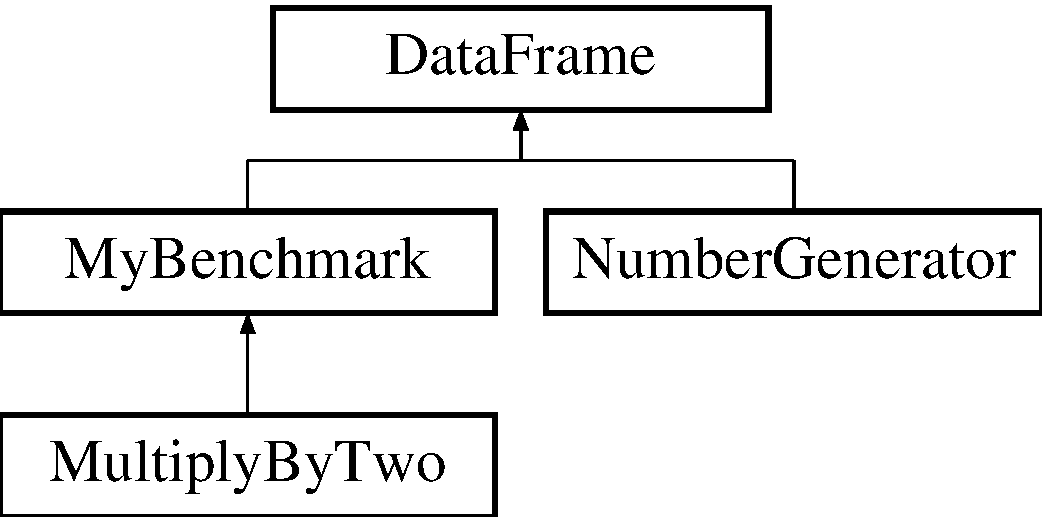
\includegraphics[height=3.000000cm]{class_data_frame}
\end{center}
\end{figure}
\subsubsection*{Metody publiczne}
\begin{DoxyCompactItemize}
\item 
\hyperlink{class_data_frame_a69a9dc47b7506b8062fd34aedacbf579}{Data\-Frame} ()
\begin{DoxyCompactList}\small\item\em Przypisuje zmiennym wartosci domyslne. \end{DoxyCompactList}\item 
int \hyperlink{class_data_frame_a617ef21804065f31115c01527155f499}{load\-Data\-From\-File} ()
\begin{DoxyCompactList}\small\item\em Ładuje dane z pliku. \end{DoxyCompactList}\item 
int \hyperlink{class_data_frame_a03cc3ac606fdb8a2dbcaea5d429cf208}{save\-Data\-To\-File} ()
\begin{DoxyCompactList}\small\item\em Zapisuje dane do pliku. \end{DoxyCompactList}\item 
\hyperlink{class_data_frame}{Data\-Frame} \hyperlink{class_data_frame_ab7dddb09f5ee9dc4a5783136dad01962}{operator=} (\hyperlink{class_data_frame}{Data\-Frame} dataframe)
\begin{DoxyCompactList}\small\item\em Kopiuje elementy roznych obiektow. \end{DoxyCompactList}\item 
virtual \hyperlink{class_data_frame_a1360ddf00d717392fe1292bc1e1990ff}{$\sim$\-Data\-Frame} ()
\end{DoxyCompactItemize}
\subsubsection*{Atrybuty publiczne}
\begin{DoxyCompactItemize}
\item 
int $\ast$ \hyperlink{class_data_frame_a8edc4ce524483e2e5069067267ccdcbf}{table\-Of\-Data}
\begin{DoxyCompactList}\small\item\em Zawiera adres do tablicy \{size\} elementów. \end{DoxyCompactList}\item 
char $\ast$ \hyperlink{class_data_frame_a824a73f019aec71281837abafd95a510}{output\-File\-Name}
\begin{DoxyCompactList}\small\item\em Zawiera nazwe pliku do zapisu. \end{DoxyCompactList}\item 
char $\ast$ \hyperlink{class_data_frame_a90041bfdf474b0d7ce39bc3dbbb55aa9}{input\-File\-Name}
\begin{DoxyCompactList}\small\item\em Zawiera nazwe pliku do odczytu. \end{DoxyCompactList}\item 
unsigned int \hyperlink{class_data_frame_aa5d1905c6910cad07ab5189bd34b13ab}{size\-Of\-Table}
\begin{DoxyCompactList}\small\item\em Rozmiar tablicy table\-Of\-Data. \end{DoxyCompactList}\end{DoxyCompactItemize}


\subsubsection{Opis szczegółowy}


Definicja w linii \hyperlink{dataframe_8h_source_l00015}{15} pliku \hyperlink{dataframe_8h_source}{dataframe.\-h}.



\subsubsection{Dokumentacja konstruktora i destruktora}
\hypertarget{class_data_frame_a69a9dc47b7506b8062fd34aedacbf579}{\index{Data\-Frame@{Data\-Frame}!Data\-Frame@{Data\-Frame}}
\index{Data\-Frame@{Data\-Frame}!DataFrame@{Data\-Frame}}
\paragraph[{Data\-Frame}]{\setlength{\rightskip}{0pt plus 5cm}Data\-Frame\-::\-Data\-Frame (
\begin{DoxyParamCaption}
{}
\end{DoxyParamCaption}
)}}\label{class_data_frame_a69a9dc47b7506b8062fd34aedacbf579}


Definicja w linii \hyperlink{dataframe_8cpp_source_l00012}{12} pliku \hyperlink{dataframe_8cpp_source}{dataframe.\-cpp}.



Odwołuje się do \hyperlink{dataframe_8h_source_l00029}{input\-File\-Name}, \hyperlink{dataframe_8h_source_l00025}{output\-File\-Name}, \hyperlink{dataframe_8h_source_l00034}{size\-Of\-Table} i \hyperlink{dataframe_8h_source_l00021}{table\-Of\-Data}.


\begin{DoxyCode}
00013 \{
00014         \hyperlink{class_data_frame_a8edc4ce524483e2e5069067267ccdcbf}{tableOfData} = 0;
00015         \hyperlink{class_data_frame_a824a73f019aec71281837abafd95a510}{outputFileName} = NULL;
00016         \hyperlink{class_data_frame_a90041bfdf474b0d7ce39bc3dbbb55aa9}{inputFileName} = NULL;
00017         \hyperlink{class_data_frame_aa5d1905c6910cad07ab5189bd34b13ab}{sizeOfTable} = 0;
00018 \}
\end{DoxyCode}
\hypertarget{class_data_frame_a1360ddf00d717392fe1292bc1e1990ff}{\index{Data\-Frame@{Data\-Frame}!$\sim$\-Data\-Frame@{$\sim$\-Data\-Frame}}
\index{$\sim$\-Data\-Frame@{$\sim$\-Data\-Frame}!DataFrame@{Data\-Frame}}
\paragraph[{$\sim$\-Data\-Frame}]{\setlength{\rightskip}{0pt plus 5cm}virtual Data\-Frame\-::$\sim$\-Data\-Frame (
\begin{DoxyParamCaption}
{}
\end{DoxyParamCaption}
)\hspace{0.3cm}{\ttfamily [inline]}, {\ttfamily [virtual]}}}\label{class_data_frame_a1360ddf00d717392fe1292bc1e1990ff}


Definicja w linii \hyperlink{dataframe_8h_source_l00064}{64} pliku \hyperlink{dataframe_8h_source}{dataframe.\-h}.


\begin{DoxyCode}
00064 \{\}
\end{DoxyCode}


\subsubsection{Dokumentacja funkcji składowych}
\hypertarget{class_data_frame_a617ef21804065f31115c01527155f499}{\index{Data\-Frame@{Data\-Frame}!load\-Data\-From\-File@{load\-Data\-From\-File}}
\index{load\-Data\-From\-File@{load\-Data\-From\-File}!DataFrame@{Data\-Frame}}
\paragraph[{load\-Data\-From\-File}]{\setlength{\rightskip}{0pt plus 5cm}int Data\-Frame\-::load\-Data\-From\-File (
\begin{DoxyParamCaption}
{}
\end{DoxyParamCaption}
)}}\label{class_data_frame_a617ef21804065f31115c01527155f499}
Wczytuje dane z pliku i zapisuje je dynamicznie do tablicy jednowymiarowej, na ktora wskazuje wskaźnik $\ast$table\-Of\-Data

Rozmiar tablicy jest przechowywany w size\-Of\-Table 

Definicja w linii \hyperlink{dataframe_8cpp_source_l00020}{20} pliku \hyperlink{dataframe_8cpp_source}{dataframe.\-cpp}.



Odwołuje się do \hyperlink{dataframe_8h_source_l00029}{input\-File\-Name}, \hyperlink{dataframe_8h_source_l00034}{size\-Of\-Table} i \hyperlink{dataframe_8h_source_l00021}{table\-Of\-Data}.


\begin{DoxyCode}
00021 \{
00022         std::ifstream streamToFile;
00023         streamToFile.open (\hyperlink{class_data_frame_a90041bfdf474b0d7ce39bc3dbbb55aa9}{inputFileName}, std::ifstream::in);
00024         this->\hyperlink{class_data_frame_a8edc4ce524483e2e5069067267ccdcbf}{tableOfData} = \textcolor{keyword}{new} \textcolor{keywordtype}{int}[\hyperlink{class_data_frame_aa5d1905c6910cad07ab5189bd34b13ab}{sizeOfTable}];
00025         \textcolor{keywordflow}{for}(\textcolor{keywordtype}{unsigned} \textcolor{keywordtype}{int} i=0; i<\hyperlink{class_data_frame_aa5d1905c6910cad07ab5189bd34b13ab}{sizeOfTable} ; i++) \{
00026                 streamToFile >> this-> \hyperlink{class_data_frame_a8edc4ce524483e2e5069067267ccdcbf}{tableOfData}[i];
00027                 \textcolor{keywordflow}{if} (streamToFile.eof()) \textcolor{keywordflow}{return} 1; \textcolor{comment}{//[EoF reached]}
00028         \}
00029         \textcolor{keywordflow}{return} 0;
00030 \}
\end{DoxyCode}
\hypertarget{class_data_frame_ab7dddb09f5ee9dc4a5783136dad01962}{\index{Data\-Frame@{Data\-Frame}!operator=@{operator=}}
\index{operator=@{operator=}!DataFrame@{Data\-Frame}}
\paragraph[{operator=}]{\setlength{\rightskip}{0pt plus 5cm}{\bf Data\-Frame} Data\-Frame\-::operator= (
\begin{DoxyParamCaption}
\item[{{\bf Data\-Frame}}]{dataframe}
\end{DoxyParamCaption}
)}}\label{class_data_frame_ab7dddb09f5ee9dc4a5783136dad01962}
Zapisuje kolejne liczby do pliku o nazwie output\-File\-Name 

Definicja w linii \hyperlink{dataframe_8cpp_source_l00044}{44} pliku \hyperlink{dataframe_8cpp_source}{dataframe.\-cpp}.



Odwołuje się do \hyperlink{dataframe_8h_source_l00029}{input\-File\-Name}, \hyperlink{dataframe_8h_source_l00025}{output\-File\-Name}, \hyperlink{dataframe_8h_source_l00034}{size\-Of\-Table} i \hyperlink{dataframe_8h_source_l00021}{table\-Of\-Data}.


\begin{DoxyCode}
00045 \{
00046         this->\hyperlink{class_data_frame_a8edc4ce524483e2e5069067267ccdcbf}{tableOfData} = dataframe.\hyperlink{class_data_frame_a8edc4ce524483e2e5069067267ccdcbf}{tableOfData};
00047         this->\hyperlink{class_data_frame_a824a73f019aec71281837abafd95a510}{outputFileName} = dataframe.\hyperlink{class_data_frame_a824a73f019aec71281837abafd95a510}{outputFileName};
00048         this->\hyperlink{class_data_frame_a90041bfdf474b0d7ce39bc3dbbb55aa9}{inputFileName} = dataframe.\hyperlink{class_data_frame_a90041bfdf474b0d7ce39bc3dbbb55aa9}{inputFileName};
00049         this->\hyperlink{class_data_frame_aa5d1905c6910cad07ab5189bd34b13ab}{sizeOfTable} = dataframe.\hyperlink{class_data_frame_aa5d1905c6910cad07ab5189bd34b13ab}{sizeOfTable};
00050         \textcolor{keywordflow}{return} *\textcolor{keyword}{this};
00051 \}
\end{DoxyCode}
\hypertarget{class_data_frame_a03cc3ac606fdb8a2dbcaea5d429cf208}{\index{Data\-Frame@{Data\-Frame}!save\-Data\-To\-File@{save\-Data\-To\-File}}
\index{save\-Data\-To\-File@{save\-Data\-To\-File}!DataFrame@{Data\-Frame}}
\paragraph[{save\-Data\-To\-File}]{\setlength{\rightskip}{0pt plus 5cm}int Data\-Frame\-::save\-Data\-To\-File (
\begin{DoxyParamCaption}
{}
\end{DoxyParamCaption}
)}}\label{class_data_frame_a03cc3ac606fdb8a2dbcaea5d429cf208}
Wczytuje liczby z pliku o nazwie intput\-File\-Name 

Definicja w linii \hyperlink{dataframe_8cpp_source_l00032}{32} pliku \hyperlink{dataframe_8cpp_source}{dataframe.\-cpp}.



Odwołuje się do \hyperlink{dataframe_8h_source_l00025}{output\-File\-Name}, \hyperlink{dataframe_8h_source_l00034}{size\-Of\-Table} i \hyperlink{dataframe_8h_source_l00021}{table\-Of\-Data}.



Odwołania w \hyperlink{main_8cpp_source_l00018}{main()}.


\begin{DoxyCode}
00033 \{
00034         std::ofstream streamToFile;
00035         streamToFile.open (\hyperlink{class_data_frame_a824a73f019aec71281837abafd95a510}{outputFileName}, std::ofstream::out);
00036         \textcolor{keywordflow}{for}(\textcolor{keywordtype}{unsigned} \textcolor{keywordtype}{int} i=0; i<\hyperlink{class_data_frame_aa5d1905c6910cad07ab5189bd34b13ab}{sizeOfTable} ; i++) \{
00037                 streamToFile << this-> \hyperlink{class_data_frame_a8edc4ce524483e2e5069067267ccdcbf}{tableOfData}[i] <<\textcolor{charliteral}{' '};
00038         \}
00039         \textcolor{keywordflow}{return} 0;
00040 \}
\end{DoxyCode}


\subsubsection{Dokumentacja atrybutów składowych}
\hypertarget{class_data_frame_a90041bfdf474b0d7ce39bc3dbbb55aa9}{\index{Data\-Frame@{Data\-Frame}!input\-File\-Name@{input\-File\-Name}}
\index{input\-File\-Name@{input\-File\-Name}!DataFrame@{Data\-Frame}}
\paragraph[{input\-File\-Name}]{\setlength{\rightskip}{0pt plus 5cm}char$\ast$ Data\-Frame\-::input\-File\-Name}}\label{class_data_frame_a90041bfdf474b0d7ce39bc3dbbb55aa9}


Definicja w linii \hyperlink{dataframe_8h_source_l00029}{29} pliku \hyperlink{dataframe_8h_source}{dataframe.\-h}.



Odwołania w \hyperlink{dataframe_8cpp_source_l00012}{Data\-Frame()}, \hyperlink{dataframe_8cpp_source_l00020}{load\-Data\-From\-File()}, \hyperlink{main_8cpp_source_l00018}{main()} i \hyperlink{dataframe_8cpp_source_l00044}{operator=()}.

\hypertarget{class_data_frame_a824a73f019aec71281837abafd95a510}{\index{Data\-Frame@{Data\-Frame}!output\-File\-Name@{output\-File\-Name}}
\index{output\-File\-Name@{output\-File\-Name}!DataFrame@{Data\-Frame}}
\paragraph[{output\-File\-Name}]{\setlength{\rightskip}{0pt plus 5cm}char$\ast$ Data\-Frame\-::output\-File\-Name}}\label{class_data_frame_a824a73f019aec71281837abafd95a510}


Definicja w linii \hyperlink{dataframe_8h_source_l00025}{25} pliku \hyperlink{dataframe_8h_source}{dataframe.\-h}.



Odwołania w \hyperlink{dataframe_8cpp_source_l00012}{Data\-Frame()}, \hyperlink{main_8cpp_source_l00018}{main()}, \hyperlink{dataframe_8cpp_source_l00044}{operator=()} i \hyperlink{dataframe_8cpp_source_l00032}{save\-Data\-To\-File()}.

\hypertarget{class_data_frame_aa5d1905c6910cad07ab5189bd34b13ab}{\index{Data\-Frame@{Data\-Frame}!size\-Of\-Table@{size\-Of\-Table}}
\index{size\-Of\-Table@{size\-Of\-Table}!DataFrame@{Data\-Frame}}
\paragraph[{size\-Of\-Table}]{\setlength{\rightskip}{0pt plus 5cm}unsigned int Data\-Frame\-::size\-Of\-Table}}\label{class_data_frame_aa5d1905c6910cad07ab5189bd34b13ab}


Definicja w linii \hyperlink{dataframe_8h_source_l00034}{34} pliku \hyperlink{dataframe_8h_source}{dataframe.\-h}.



Odwołania w \hyperlink{dataframe_8cpp_source_l00012}{Data\-Frame()}, \hyperlink{multiplybytwo_8cpp_source_l00011}{Multiply\-By\-Two\-::execute\-Algorithm()}, \hyperlink{numbergenerator_8h_source_l00035}{Number\-Generator\-::generate\-Numbers()}, \hyperlink{numbergenerator_8cpp_source_l00010}{Number\-Generator\-::generate\-Strings()}, \hyperlink{dataframe_8cpp_source_l00020}{load\-Data\-From\-File()}, \hyperlink{main_8cpp_source_l00018}{main()}, \hyperlink{dataframe_8cpp_source_l00044}{operator=()}, \hyperlink{dataframe_8cpp_source_l00032}{save\-Data\-To\-File()} i \hyperlink{mybenchmark_8cpp_source_l00012}{My\-Benchmark\-::test\-Algorithm()}.

\hypertarget{class_data_frame_a8edc4ce524483e2e5069067267ccdcbf}{\index{Data\-Frame@{Data\-Frame}!table\-Of\-Data@{table\-Of\-Data}}
\index{table\-Of\-Data@{table\-Of\-Data}!DataFrame@{Data\-Frame}}
\paragraph[{table\-Of\-Data}]{\setlength{\rightskip}{0pt plus 5cm}int$\ast$ Data\-Frame\-::table\-Of\-Data}}\label{class_data_frame_a8edc4ce524483e2e5069067267ccdcbf}


Definicja w linii \hyperlink{dataframe_8h_source_l00021}{21} pliku \hyperlink{dataframe_8h_source}{dataframe.\-h}.



Odwołania w \hyperlink{dataframe_8cpp_source_l00012}{Data\-Frame()}, \hyperlink{multiplybytwo_8cpp_source_l00011}{Multiply\-By\-Two\-::execute\-Algorithm()}, \hyperlink{numbergenerator_8h_source_l00035}{Number\-Generator\-::generate\-Numbers()}, \hyperlink{numbergenerator_8cpp_source_l00010}{Number\-Generator\-::generate\-Strings()}, \hyperlink{dataframe_8cpp_source_l00020}{load\-Data\-From\-File()}, \hyperlink{main_8cpp_source_l00018}{main()}, \hyperlink{dataframe_8cpp_source_l00044}{operator=()}, \hyperlink{dataframe_8cpp_source_l00032}{save\-Data\-To\-File()} i \hyperlink{mybenchmark_8cpp_source_l00012}{My\-Benchmark\-::test\-Algorithm()}.



Dokumentacja dla tej klasy została wygenerowana z plików\-:\begin{DoxyCompactItemize}
\item 
\hyperlink{dataframe_8h}{dataframe.\-h}\item 
\hyperlink{dataframe_8cpp}{dataframe.\-cpp}\end{DoxyCompactItemize}

\hypertarget{class_dictionary}{\subsection{Dokumentacja klasy Dictionary}
\label{class_dictionary}\index{Dictionary@{Dictionary}}
}


Klasa tworzy tablicy asocjacyjną -\/ słownik.  




{\ttfamily \#include $<$dictionary.\-h$>$}

\subsubsection*{Metody publiczne}
\begin{DoxyCompactItemize}
\item 
\hyperlink{class_dictionary_aee8d612bc9d323c38faba045ba384b8b}{Dictionary} ()
\begin{DoxyCompactList}\small\item\em Konstruktor tworzacy kolumne\-List Tworze 367 miejsc bo mam tylko trzy pierwsze znaki uzywane przy hashowaniu. \end{DoxyCompactList}\item 
int \& \hyperlink{class_dictionary_a5a82ede9a412aa8a9b7bee9b2a423427}{operator\mbox{[}$\,$\mbox{]}} (string str)
\begin{DoxyCompactList}\small\item\em Operator pozwalajacy odnosic sie do slownika Gdy element o danym kluczu nie istnieje, a użytkownik próbuje sie do niego odwołać to dany element jest tworzony i dodawany do tablicy. \end{DoxyCompactList}\end{DoxyCompactItemize}
\subsubsection*{Statyczne metody publiczne}
\begin{DoxyCompactItemize}
\item 
static int \hyperlink{class_dictionary_a53981ac20e3ab2b7544d6f6f3111cdf4}{str2int} (string str)
\begin{DoxyCompactList}\small\item\em Funkcja hashująca trzy pierwsze znaki. \end{DoxyCompactList}\item 
static int \hyperlink{class_dictionary_a7dd06f1225844c860a73d98b8a814da7}{str2int\-All} (string str)
\begin{DoxyCompactList}\small\item\em Funkcja hashująca wszystkie znaki. \end{DoxyCompactList}\end{DoxyCompactItemize}
\subsubsection*{Atrybuty prywatne}
\begin{DoxyCompactItemize}
\item 
\hyperlink{class_my_list}{My\-List} $\ast$ \hyperlink{class_dictionary_a36adbe694dbbdcbd577d9e8486bdf40a}{kolumna\-List}
\begin{DoxyCompactList}\small\item\em Tablica list. \end{DoxyCompactList}\end{DoxyCompactItemize}


\subsubsection{Opis szczegółowy}
Tworzy tablice asocjacyjną, na podstawie kluczba podanego przez operator \mbox{[}\mbox{]} Gdy element o danym kluczu nie istnieje, a użytkownik próbuje sie do niego odwołać to dany element jest tworzony i dodawany do tablicy 

Definicja w linii \hyperlink{dictionary_8h_source_l00025}{25} pliku \hyperlink{dictionary_8h_source}{dictionary.\-h}.



\subsubsection{Dokumentacja konstruktora i destruktora}
\hypertarget{class_dictionary_aee8d612bc9d323c38faba045ba384b8b}{\index{Dictionary@{Dictionary}!Dictionary@{Dictionary}}
\index{Dictionary@{Dictionary}!Dictionary@{Dictionary}}
\paragraph[{Dictionary}]{\setlength{\rightskip}{0pt plus 5cm}Dictionary\-::\-Dictionary (
\begin{DoxyParamCaption}
{}
\end{DoxyParamCaption}
)\hspace{0.3cm}{\ttfamily [inline]}}}\label{class_dictionary_aee8d612bc9d323c38faba045ba384b8b}


Definicja w linii \hyperlink{dictionary_8h_source_l00037}{37} pliku \hyperlink{dictionary_8h_source}{dictionary.\-h}.



Odwołuje się do \hyperlink{dictionary_8h_source_l00010}{L\-I\-C\-Z\-B\-A\-\_\-\-Z\-N\-A\-K\-O\-W\-\_\-\-D\-O\-\_\-\-H\-A\-S\-H\-U} i \hyperlink{numbergenerator_8h_source_l00017}{M\-A\-X\-\_\-\-H\-E\-X\-\_\-\-A\-S\-C\-I\-I\-\_\-\-K\-O\-D}.


\begin{DoxyCode}
00037 \{       \hyperlink{class_dictionary_a36adbe694dbbdcbd577d9e8486bdf40a}{kolumnaList} = \textcolor{keyword}{new} \hyperlink{class_my_list}{MyList}[ \hyperlink{dictionary_8h_a562499e66e3ed9cc37111ac1ddafa1eb}{LICZBA\_ZNAKOW\_DO\_HASHU} * 
      \hyperlink{numbergenerator_8h_ad234b171c744b5f476c1685da37bb7ca}{MAX\_HEX\_ASCII\_KOD}+1]; \}
\end{DoxyCode}


\subsubsection{Dokumentacja funkcji składowych}
\hypertarget{class_dictionary_a5a82ede9a412aa8a9b7bee9b2a423427}{\index{Dictionary@{Dictionary}!operator\mbox{[}$\,$\mbox{]}@{operator[]}}
\index{operator\mbox{[}$\,$\mbox{]}@{operator[]}!Dictionary@{Dictionary}}
\paragraph[{operator[]}]{\setlength{\rightskip}{0pt plus 5cm}int \& Dictionary\-::operator\mbox{[}$\,$\mbox{]} (
\begin{DoxyParamCaption}
\item[{string}]{str}
\end{DoxyParamCaption}
)}}\label{class_dictionary_a5a82ede9a412aa8a9b7bee9b2a423427}

\begin{DoxyParams}{Parametry}
{\em str} & Klucz elementu do odwolania \\
\hline
\end{DoxyParams}


Definicja w linii \hyperlink{dictionary_8cpp_source_l00011}{11} pliku \hyperlink{dictionary_8cpp_source}{dictionary.\-cpp}.



Odwołuje się do \hyperlink{dictionary_8h_source_l00030}{kolumna\-List}, \hyperlink{mylist_8h_source_l00030}{My\-List\-::\-My\-List\-Element\-::nazwa}, \hyperlink{mylist_8h_source_l00029}{My\-List\-::\-My\-List\-Element\-::number}, \hyperlink{mylist_8cpp_source_l00044}{My\-List\-::pop\-\_\-back()}, \hyperlink{mylist_8cpp_source_l00053}{My\-List\-::pop\-\_\-front()}, \hyperlink{mylist_8cpp_source_l00034}{My\-List\-::push\-\_\-front()}, \hyperlink{mylist_8cpp_source_l00079}{My\-List\-::show\-\_\-front()}, \hyperlink{mylist_8cpp_source_l00086}{My\-List\-::size()} i \hyperlink{dictionary_8cpp_source_l00051}{str2int()}.


\begin{DoxyCode}
00012         \{
00013                 \hyperlink{class_my_list}{MyList} tmpList;
00014                 \hyperlink{class_my_list_1_1_my_list_element}{MyList::MyListElement} tmpListElement;
00015                 \textcolor{keywordtype}{int} \textcolor{keywordtype}{id} = \hyperlink{class_dictionary_a53981ac20e3ab2b7544d6f6f3111cdf4}{str2int}(str);
00016                 \textcolor{comment}{// jezeli sa elementy na liscie}
00017                 \textcolor{comment}{//std::cerr<<"\(\backslash\)nSize listy na wejsciu do funkcji []: "<<kolumnaList[id].size();}
00018                 \textcolor{keywordflow}{while}(\hyperlink{class_dictionary_a36adbe694dbbdcbd577d9e8486bdf40a}{kolumnaList}[\textcolor{keywordtype}{id}].size())
00019                 \{
00020                 \textcolor{comment}{//std::cerr<<"\(\backslash\)nSize listy na wejsciu do while I []: "<<kolumnaList[id].size();}
00021                 \textcolor{comment}{//std::cerr<<"\(\backslash\)nhash id:"<<id;}
00022                 tmpListElement = \hyperlink{class_dictionary_a36adbe694dbbdcbd577d9e8486bdf40a}{kolumnaList}[id].\hyperlink{class_my_list_a84369accd705913f85b770770f06767a}{pop\_front}();
00023                 \textcolor{comment}{//std::cerr<<"\(\backslash\)nWyjalem klucz z liczba: "<<tmpListElement.number;}
00024                         \textcolor{keywordflow}{if}( !(tmpListElement.\hyperlink{class_my_list_1_1_my_list_element_af610aeae835150be1a12d538e67a579c}{nazwa}.compare(str)) ) \textcolor{comment}{// znalazlem taki sam klucz w
       slowniku}
00025                                 \{
00026                                 \textcolor{comment}{//std::cerr<<"\(\backslash\)nZnalazlem takie same klucze";}
00027                                         \textcolor{keywordflow}{while}(tmpList.\hyperlink{class_my_list_a6d21c8bfbd9cd31efdba81ba488f43f2}{size}())
00028                                         \{
00029                                                 \hyperlink{class_dictionary_a36adbe694dbbdcbd577d9e8486bdf40a}{kolumnaList}[id].
      \hyperlink{class_my_list_ac703cd9be1c465722e683dbdcececa6b}{push\_front}(tmpList.\hyperlink{class_my_list_afc006104d8156154ad3849d0e4cc6109}{pop\_back}());
00030                                         \}
00031                                         \hyperlink{class_dictionary_a36adbe694dbbdcbd577d9e8486bdf40a}{kolumnaList}[id].\hyperlink{class_my_list_ac703cd9be1c465722e683dbdcececa6b}{push\_front}(tmpListElement);
00032                                         \textcolor{keywordflow}{return} (\hyperlink{class_dictionary_a36adbe694dbbdcbd577d9e8486bdf40a}{kolumnaList}[\textcolor{keywordtype}{id}]).show\_front().number;
00033                                 \}
00034                         \textcolor{keywordflow}{else}
00035                         \{
00036                                 tmpList.\hyperlink{class_my_list_ac703cd9be1c465722e683dbdcececa6b}{push\_front}(tmpListElement);
00037                         \}
00038                 \}
00039                 \textcolor{comment}{//Czyli nie znalazlem takiego elementu, to go tworze}
00040                 tmpListElement.\hyperlink{class_my_list_1_1_my_list_element_acd6dbb6a8791f034f94678d46395b366}{number}=0;
00041                 tmpListElement.\hyperlink{class_my_list_1_1_my_list_element_af610aeae835150be1a12d538e67a579c}{nazwa}=str;
00042                 tmpList.\hyperlink{class_my_list_ac703cd9be1c465722e683dbdcececa6b}{push\_front}(tmpListElement);
00043                 \hyperlink{class_dictionary_a36adbe694dbbdcbd577d9e8486bdf40a}{kolumnaList}[id] = tmpList;
00044                 \textcolor{comment}{//std::cerr<<"\(\backslash\)nZapisalem nowy element: "<<kolumnaList[id].show\_front().number;}
00045                 \textcolor{keywordflow}{return} \hyperlink{class_dictionary_a36adbe694dbbdcbd577d9e8486bdf40a}{kolumnaList}[id].\hyperlink{class_my_list_a9d7990c6a8b96d4c0d267fe46582fd6b}{show\_front}().\hyperlink{class_my_list_1_1_my_list_element_acd6dbb6a8791f034f94678d46395b366}{number};
00046         \}
\end{DoxyCode}
\hypertarget{class_dictionary_a53981ac20e3ab2b7544d6f6f3111cdf4}{\index{Dictionary@{Dictionary}!str2int@{str2int}}
\index{str2int@{str2int}!Dictionary@{Dictionary}}
\paragraph[{str2int}]{\setlength{\rightskip}{0pt plus 5cm}int Dictionary\-::str2int (
\begin{DoxyParamCaption}
\item[{string}]{str}
\end{DoxyParamCaption}
)\hspace{0.3cm}{\ttfamily [static]}}}\label{class_dictionary_a53981ac20e3ab2b7544d6f6f3111cdf4}

\begin{DoxyParams}{Parametry}
{\em str} & Obiekt string do zhashowania \\
\hline
\end{DoxyParams}


Definicja w linii \hyperlink{dictionary_8cpp_source_l00051}{51} pliku \hyperlink{dictionary_8cpp_source}{dictionary.\-cpp}.



Odwołuje się do \hyperlink{dictionary_8h_source_l00010}{L\-I\-C\-Z\-B\-A\-\_\-\-Z\-N\-A\-K\-O\-W\-\_\-\-D\-O\-\_\-\-H\-A\-S\-H\-U}.



Odwołania w \hyperlink{dictionary_8cpp_source_l00011}{operator\mbox{[}$\,$\mbox{]}()}.


\begin{DoxyCode}
00051                                          \{
00052                 \textcolor{keywordtype}{int} hash=0;
00053                 \textcolor{keywordflow}{for}(\textcolor{keywordtype}{unsigned} \textcolor{keywordtype}{int} i=0; ( i<\hyperlink{dictionary_8h_a562499e66e3ed9cc37111ac1ddafa1eb}{LICZBA\_ZNAKOW\_DO\_HASHU} && i<str.size() );i+
      +)
00054                         hash += (\textcolor{keywordtype}{int})str[i];
00055                 \textcolor{comment}{//std::cout<<"\(\backslash\)nHash:"<<hash;}
00056                 \textcolor{keywordflow}{return} hash;
00057         \}
\end{DoxyCode}
\hypertarget{class_dictionary_a7dd06f1225844c860a73d98b8a814da7}{\index{Dictionary@{Dictionary}!str2int\-All@{str2int\-All}}
\index{str2int\-All@{str2int\-All}!Dictionary@{Dictionary}}
\paragraph[{str2int\-All}]{\setlength{\rightskip}{0pt plus 5cm}static int Dictionary\-::str2int\-All (
\begin{DoxyParamCaption}
\item[{string}]{str}
\end{DoxyParamCaption}
)\hspace{0.3cm}{\ttfamily [static]}}}\label{class_dictionary_a7dd06f1225844c860a73d98b8a814da7}

\begin{DoxyParams}{Parametry}
{\em str} & Obiekt string do zhashowania \\
\hline
\end{DoxyParams}


\subsubsection{Dokumentacja atrybutów składowych}
\hypertarget{class_dictionary_a36adbe694dbbdcbd577d9e8486bdf40a}{\index{Dictionary@{Dictionary}!kolumna\-List@{kolumna\-List}}
\index{kolumna\-List@{kolumna\-List}!Dictionary@{Dictionary}}
\paragraph[{kolumna\-List}]{\setlength{\rightskip}{0pt plus 5cm}{\bf My\-List}$\ast$ Dictionary\-::kolumna\-List\hspace{0.3cm}{\ttfamily [private]}}}\label{class_dictionary_a36adbe694dbbdcbd577d9e8486bdf40a}


Definicja w linii \hyperlink{dictionary_8h_source_l00030}{30} pliku \hyperlink{dictionary_8h_source}{dictionary.\-h}.



Odwołania w \hyperlink{dictionary_8cpp_source_l00011}{operator\mbox{[}$\,$\mbox{]}()}.



Dokumentacja dla tej klasy została wygenerowana z plików\-:\begin{DoxyCompactItemize}
\item 
\hyperlink{dictionary_8h}{dictionary.\-h}\item 
\hyperlink{dictionary_8cpp}{dictionary.\-cpp}\end{DoxyCompactItemize}

\hypertarget{class_hashowanie}{\subsection{Dokumentacja klasy Hashowanie}
\label{class_hashowanie}\index{Hashowanie@{Hashowanie}}
}


{\ttfamily \#include $<$hashowanie.\-h$>$}

\subsubsection*{Statyczne metody publiczne}
\begin{DoxyCompactItemize}
\item 
static int \hyperlink{class_hashowanie_a110b055bf2be74d6588c9ff20baddbbb}{str2int} (const char $\ast$str)
\end{DoxyCompactItemize}


\subsubsection{Opis szczegółowy}


Definicja w linii \hyperlink{hashowanie_8h_source_l00013}{13} pliku \hyperlink{hashowanie_8h_source}{hashowanie.\-h}.



\subsubsection{Dokumentacja funkcji składowych}
\hypertarget{class_hashowanie_a110b055bf2be74d6588c9ff20baddbbb}{\index{Hashowanie@{Hashowanie}!str2int@{str2int}}
\index{str2int@{str2int}!Hashowanie@{Hashowanie}}
\paragraph[{str2int}]{\setlength{\rightskip}{0pt plus 5cm}static int Hashowanie\-::str2int (
\begin{DoxyParamCaption}
\item[{const char $\ast$}]{str}
\end{DoxyParamCaption}
)\hspace{0.3cm}{\ttfamily [inline]}, {\ttfamily [static]}}}\label{class_hashowanie_a110b055bf2be74d6588c9ff20baddbbb}


Definicja w linii \hyperlink{hashowanie_8h_source_l00016}{16} pliku \hyperlink{hashowanie_8h_source}{hashowanie.\-h}.


\begin{DoxyCode}
00016                                            \{
00017                 \textcolor{keywordtype}{int} hash;
00018                 hash = (int)str[0]+(\textcolor{keywordtype}{int})str[1]+(int)str[2];
00019                 std::cout<<\textcolor{stringliteral}{"\(\backslash\)nHash:"}<<hash;
00020                 \textcolor{keywordflow}{return} hash;
00021         \}
\end{DoxyCode}


Dokumentacja dla tej klasy została wygenerowana z pliku\-:\begin{DoxyCompactItemize}
\item 
\hyperlink{hashowanie_8h}{hashowanie.\-h}\end{DoxyCompactItemize}

\input{class_multiply_by_two}
\hypertarget{class_my_benchmark}{\subsection{Dokumentacja klasy My\-Benchmark}
\label{class_my_benchmark}\index{My\-Benchmark@{My\-Benchmark}}
}


Klasa bazowa/interface do testowania algorytmu.  




{\ttfamily \#include $<$mybenchmark.\-h$>$}

Diagram dziedziczenia dla My\-Benchmark\begin{figure}[H]
\begin{center}
\leavevmode
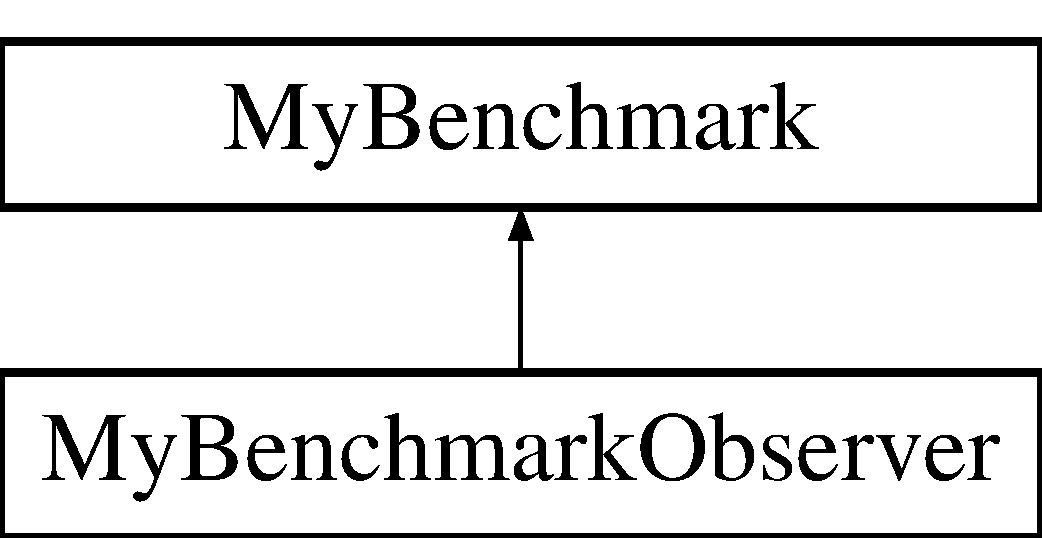
\includegraphics[height=2.000000cm]{class_my_benchmark}
\end{center}
\end{figure}
\subsubsection*{Metody publiczne}
\begin{DoxyCompactItemize}
\item 
\hyperlink{class_my_benchmark_a7f3739e8b61939627c0f63948a9975ca}{My\-Benchmark} ()
\item 
virtual \hyperlink{class_my_benchmark_a00de82c40680b41065eb402ac90f1736}{$\sim$\-My\-Benchmark} ()
\begin{DoxyCompactList}\small\item\em Usuwam obiekt test biorąc pod uwage jego prawdziwy typ. \end{DoxyCompactList}\end{DoxyCompactItemize}
\subsubsection*{Statyczne metody publiczne}
\begin{DoxyCompactItemize}
\item 
static void \hyperlink{class_my_benchmark_a802577db97fd440a3920add30c35a676}{timer\-Start} ()
\begin{DoxyCompactList}\small\item\em włączam stoper \end{DoxyCompactList}\item 
static double \hyperlink{class_my_benchmark_a7e3fa28fab999435bd4c51d915e42809}{timer\-Stop} ()
\begin{DoxyCompactList}\small\item\em wyłączam stoper \end{DoxyCompactList}\end{DoxyCompactItemize}
\subsubsection*{Atrybuty publiczne}
\begin{DoxyCompactItemize}
\item 
double \hyperlink{class_my_benchmark_a1cdab837ead670bd438f249ee82c8eff}{timer\-Value}
\begin{DoxyCompactList}\small\item\em Interface metody algorytmu glownego. \end{DoxyCompactList}\item 
std\-::ofstream \hyperlink{class_my_benchmark_a45b39f704800f8403789ff5c9bbb486b}{stream\-To\-File}
\end{DoxyCompactItemize}
\subsubsection*{Statyczne atrybuty publiczne}
\begin{DoxyCompactItemize}
\item 
static double \hyperlink{class_my_benchmark_aeca64d5b265e357ef879bf982dd4bb00}{timer\-Value\-Static} =0
\end{DoxyCompactItemize}


\subsubsection{Opis szczegółowy}
Używana jako interface dla wszystkich algorytmow aby testowac czas wykonywanego algorymtu. 

Definicja w linii \hyperlink{mybenchmark_8h_source_l00023}{23} pliku \hyperlink{mybenchmark_8h_source}{mybenchmark.\-h}.



\subsubsection{Dokumentacja konstruktora i destruktora}
\hypertarget{class_my_benchmark_a7f3739e8b61939627c0f63948a9975ca}{\index{My\-Benchmark@{My\-Benchmark}!My\-Benchmark@{My\-Benchmark}}
\index{My\-Benchmark@{My\-Benchmark}!MyBenchmark@{My\-Benchmark}}
\paragraph[{My\-Benchmark}]{\setlength{\rightskip}{0pt plus 5cm}My\-Benchmark\-::\-My\-Benchmark (
\begin{DoxyParamCaption}
{}
\end{DoxyParamCaption}
)\hspace{0.3cm}{\ttfamily [inline]}}}\label{class_my_benchmark_a7f3739e8b61939627c0f63948a9975ca}


Definicja w linii \hyperlink{mybenchmark_8h_source_l00043}{43} pliku \hyperlink{mybenchmark_8h_source}{mybenchmark.\-h}.



Odwołuje się do \hyperlink{mybenchmark_8h_source_l00041}{stream\-To\-File} i \hyperlink{mybenchmark_8h_source_l00040}{timer\-Value}.


\begin{DoxyCode}
00044         \{
00045                 \hyperlink{class_my_benchmark_a1cdab837ead670bd438f249ee82c8eff}{timerValue} = 0;
00046                 \hyperlink{class_my_benchmark_a45b39f704800f8403789ff5c9bbb486b}{streamToFile}.open (\textcolor{stringliteral}{"log.txt"}, std::ofstream::out  | std::ofstream::trunc);
00047                         \hyperlink{class_my_benchmark_a45b39f704800f8403789ff5c9bbb486b}{streamToFile}.close();
00048                 \hyperlink{class_my_benchmark_a45b39f704800f8403789ff5c9bbb486b}{streamToFile}.open (\textcolor{stringliteral}{"log.txt"}, std::ofstream::app);
00049                 \hyperlink{class_my_benchmark_a45b39f704800f8403789ff5c9bbb486b}{streamToFile} << std::fixed;
00050         \}
\end{DoxyCode}
\hypertarget{class_my_benchmark_a00de82c40680b41065eb402ac90f1736}{\index{My\-Benchmark@{My\-Benchmark}!$\sim$\-My\-Benchmark@{$\sim$\-My\-Benchmark}}
\index{$\sim$\-My\-Benchmark@{$\sim$\-My\-Benchmark}!MyBenchmark@{My\-Benchmark}}
\paragraph[{$\sim$\-My\-Benchmark}]{\setlength{\rightskip}{0pt plus 5cm}virtual My\-Benchmark\-::$\sim$\-My\-Benchmark (
\begin{DoxyParamCaption}
{}
\end{DoxyParamCaption}
)\hspace{0.3cm}{\ttfamily [inline]}, {\ttfamily [virtual]}}}\label{class_my_benchmark_a00de82c40680b41065eb402ac90f1736}


Definicja w linii \hyperlink{mybenchmark_8h_source_l00066}{66} pliku \hyperlink{mybenchmark_8h_source}{mybenchmark.\-h}.


\begin{DoxyCode}
00066 \{\};
\end{DoxyCode}


\subsubsection{Dokumentacja funkcji składowych}
\hypertarget{class_my_benchmark_a802577db97fd440a3920add30c35a676}{\index{My\-Benchmark@{My\-Benchmark}!timer\-Start@{timer\-Start}}
\index{timer\-Start@{timer\-Start}!MyBenchmark@{My\-Benchmark}}
\paragraph[{timer\-Start}]{\setlength{\rightskip}{0pt plus 5cm}void My\-Benchmark\-::timer\-Start (
\begin{DoxyParamCaption}
{}
\end{DoxyParamCaption}
)\hspace{0.3cm}{\ttfamily [static]}}}\label{class_my_benchmark_a802577db97fd440a3920add30c35a676}


Definicja w linii \hyperlink{mybenchmark_8cpp_source_l00012}{12} pliku \hyperlink{mybenchmark_8cpp_source}{mybenchmark.\-cpp}.



Odwołuje się do \hyperlink{mybenchmark_8h_source_l00042}{timer\-Value\-Static}.



Odwołania w \hyperlink{mybenchmark_8h_source_l00077}{My\-Benchmark\-Observer\-::received\-Start\-Update()}.


\begin{DoxyCode}
00013 \{
00014         \hyperlink{class_my_benchmark_aeca64d5b265e357ef879bf982dd4bb00}{MyBenchmark::timerValueStatic} = (( (double)clock() ) /CLOCKS\_PER\_SEC);
00015 \}
\end{DoxyCode}
\hypertarget{class_my_benchmark_a7e3fa28fab999435bd4c51d915e42809}{\index{My\-Benchmark@{My\-Benchmark}!timer\-Stop@{timer\-Stop}}
\index{timer\-Stop@{timer\-Stop}!MyBenchmark@{My\-Benchmark}}
\paragraph[{timer\-Stop}]{\setlength{\rightskip}{0pt plus 5cm}double My\-Benchmark\-::timer\-Stop (
\begin{DoxyParamCaption}
{}
\end{DoxyParamCaption}
)\hspace{0.3cm}{\ttfamily [static]}}}\label{class_my_benchmark_a7e3fa28fab999435bd4c51d915e42809}
\begin{DoxyReturn}{Zwraca}
Dlugosc dzialania stopera 
\end{DoxyReturn}


Definicja w linii \hyperlink{mybenchmark_8cpp_source_l00017}{17} pliku \hyperlink{mybenchmark_8cpp_source}{mybenchmark.\-cpp}.



Odwołuje się do \hyperlink{mybenchmark_8h_source_l00042}{timer\-Value\-Static}.



Odwołania w \hyperlink{mybenchmark_8h_source_l00082}{My\-Benchmark\-Observer\-::received\-Stop\-Update()} i \hyperlink{mybenchmark_8h_source_l00086}{My\-Benchmark\-Observer\-::received\-Stop\-Update\-And\-Save\-To\-File()}.


\begin{DoxyCode}
00018 \{
00019         \textcolor{keywordflow}{return} (( (\textcolor{keywordtype}{double})clock() ) /CLOCKS\_PER\_SEC) - 
      \hyperlink{class_my_benchmark_aeca64d5b265e357ef879bf982dd4bb00}{MyBenchmark::timerValueStatic};
00020 \}
\end{DoxyCode}


\subsubsection{Dokumentacja atrybutów składowych}
\hypertarget{class_my_benchmark_a45b39f704800f8403789ff5c9bbb486b}{\index{My\-Benchmark@{My\-Benchmark}!stream\-To\-File@{stream\-To\-File}}
\index{stream\-To\-File@{stream\-To\-File}!MyBenchmark@{My\-Benchmark}}
\paragraph[{stream\-To\-File}]{\setlength{\rightskip}{0pt plus 5cm}std\-::ofstream My\-Benchmark\-::stream\-To\-File}}\label{class_my_benchmark_a45b39f704800f8403789ff5c9bbb486b}


Definicja w linii \hyperlink{mybenchmark_8h_source_l00041}{41} pliku \hyperlink{mybenchmark_8h_source}{mybenchmark.\-h}.



Odwołania w \hyperlink{mybenchmark_8h_source_l00043}{My\-Benchmark()}, \hyperlink{mybenchmark_8h_source_l00086}{My\-Benchmark\-Observer\-::received\-Stop\-Update\-And\-Save\-To\-File()} i \hyperlink{mybenchmark_8h_source_l00092}{My\-Benchmark\-Observer\-::$\sim$\-My\-Benchmark\-Observer()}.

\hypertarget{class_my_benchmark_a1cdab837ead670bd438f249ee82c8eff}{\index{My\-Benchmark@{My\-Benchmark}!timer\-Value@{timer\-Value}}
\index{timer\-Value@{timer\-Value}!MyBenchmark@{My\-Benchmark}}
\paragraph[{timer\-Value}]{\setlength{\rightskip}{0pt plus 5cm}double My\-Benchmark\-::timer\-Value}}\label{class_my_benchmark_a1cdab837ead670bd438f249ee82c8eff}
Metoda abstrakcyjna, ktora jest interfacem do implementacji przez glowny algorytm. To znaczy, ze kazdy algorytm ma byc uruchamiany tą funkcja\-Czas stopera 

Definicja w linii \hyperlink{mybenchmark_8h_source_l00040}{40} pliku \hyperlink{mybenchmark_8h_source}{mybenchmark.\-h}.



Odwołania w \hyperlink{mybenchmark_8h_source_l00076}{My\-Benchmark\-Observer\-::get\-Timer\-Value()}, \hyperlink{mybenchmark_8h_source_l00043}{My\-Benchmark()} i \hyperlink{mybenchmark_8h_source_l00086}{My\-Benchmark\-Observer\-::received\-Stop\-Update\-And\-Save\-To\-File()}.

\hypertarget{class_my_benchmark_aeca64d5b265e357ef879bf982dd4bb00}{\index{My\-Benchmark@{My\-Benchmark}!timer\-Value\-Static@{timer\-Value\-Static}}
\index{timer\-Value\-Static@{timer\-Value\-Static}!MyBenchmark@{My\-Benchmark}}
\paragraph[{timer\-Value\-Static}]{\setlength{\rightskip}{0pt plus 5cm}double My\-Benchmark\-::timer\-Value\-Static =0\hspace{0.3cm}{\ttfamily [static]}}}\label{class_my_benchmark_aeca64d5b265e357ef879bf982dd4bb00}


Definicja w linii \hyperlink{mybenchmark_8h_source_l00042}{42} pliku \hyperlink{mybenchmark_8h_source}{mybenchmark.\-h}.



Odwołania w \hyperlink{mybenchmark_8cpp_source_l00012}{timer\-Start()} i \hyperlink{mybenchmark_8cpp_source_l00017}{timer\-Stop()}.



Dokumentacja dla tej klasy została wygenerowana z plików\-:\begin{DoxyCompactItemize}
\item 
\hyperlink{mybenchmark_8h}{mybenchmark.\-h}\item 
\hyperlink{mybenchmark_8cpp}{mybenchmark.\-cpp}\end{DoxyCompactItemize}

\hypertarget{class_my_list}{\subsection{Dokumentacja klasy My\-List}
\label{class_my_list}\index{My\-List@{My\-List}}
}


Lista dwukierunkowa.  




{\ttfamily \#include $<$mylist.\-h$>$}

Diagram dziedziczenia dla My\-List\begin{figure}[H]
\begin{center}
\leavevmode
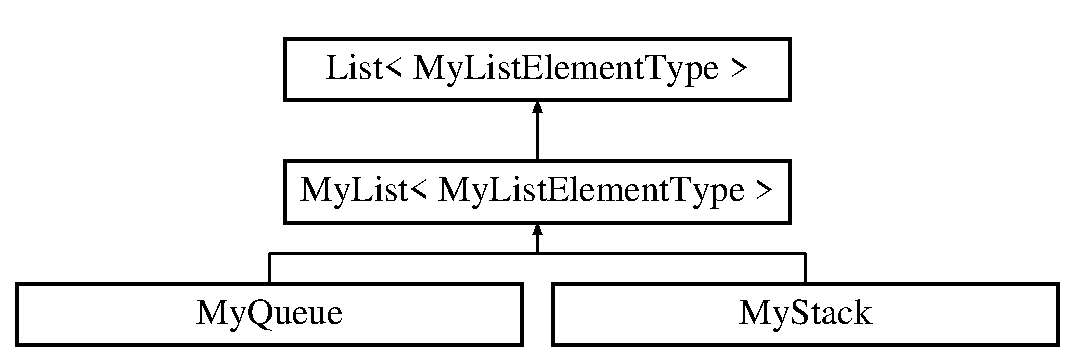
\includegraphics[height=2.000000cm]{class_my_list}
\end{center}
\end{figure}
\subsubsection*{Komponenty}
\begin{DoxyCompactItemize}
\item 
class \hyperlink{class_my_list_1_1_my_list_element}{My\-List\-Element}
\begin{DoxyCompactList}\small\item\em Klasa 'malych struktur' gdzie jest numer i wskaznik do nas elementu. \end{DoxyCompactList}\end{DoxyCompactItemize}
\subsubsection*{Metody publiczne}
\begin{DoxyCompactItemize}
\item 
\hyperlink{class_my_list_ae9cd2a6b068e02fa39ba3e539425c1c1}{My\-List} ()
\begin{DoxyCompactList}\small\item\em Konstruktor listy. \end{DoxyCompactList}\item 
int \hyperlink{class_my_list_a6d21c8bfbd9cd31efdba81ba488f43f2}{size} ()
\begin{DoxyCompactList}\small\item\em Zwraca ilosc elementow listy. \end{DoxyCompactList}\item 
\hyperlink{class_my_list_1_1_my_list_element}{My\-List\-Element} \hyperlink{class_my_list_afc006104d8156154ad3849d0e4cc6109}{pop\-\_\-back} ()
\begin{DoxyCompactList}\small\item\em Zwraca element ostatni w liscie. \end{DoxyCompactList}\item 
\hyperlink{class_my_list_1_1_my_list_element}{My\-List\-Element} \hyperlink{class_my_list_a84369accd705913f85b770770f06767a}{pop\-\_\-front} ()
\begin{DoxyCompactList}\small\item\em Zwraca element pierwszy w liscie. \end{DoxyCompactList}\item 
void \hyperlink{class_my_list_a06c2749553f559eb3d5d227e0ac07c53}{push\-\_\-back} (\hyperlink{class_my_list_1_1_my_list_element}{My\-List\-Element} arg)
\begin{DoxyCompactList}\small\item\em Wklada element na ostatnie miejsce na liscie. \end{DoxyCompactList}\item 
void \hyperlink{class_my_list_ac703cd9be1c465722e683dbdcececa6b}{push\-\_\-front} (\hyperlink{class_my_list_1_1_my_list_element}{My\-List\-Element} arg)
\begin{DoxyCompactList}\small\item\em Wklada element na pierwsze miejsce na liscie. \end{DoxyCompactList}\item 
\hyperlink{class_my_list_1_1_my_list_element}{My\-List\-Element} \& \hyperlink{class_my_list_a9d7990c6a8b96d4c0d267fe46582fd6b}{show\-\_\-front} ()
\begin{DoxyCompactList}\small\item\em Pokazuje element po poczatku listy. \end{DoxyCompactList}\item 
\hyperlink{class_my_list_1_1_my_list_element}{My\-List\-Element} \& \hyperlink{class_my_list_ab67b7b37e96d5cb31742efbdf283fa9f}{show\-\_\-back} ()
\begin{DoxyCompactList}\small\item\em Pokazuje element po koncu listy. \end{DoxyCompactList}\item 
int \hyperlink{class_my_list_a94a6183f4d3248ca593b51a173bd2d50}{save\-Data\-To\-File} ()
\end{DoxyCompactItemize}
\subsubsection*{Atrybuty publiczne}
\begin{DoxyCompactItemize}
\item 
\hyperlink{class_my_list_1_1_my_list_element}{My\-List\-Element} $\ast$ \hyperlink{class_my_list_aa7e5ddd2dddeeccd304126130d73dead}{first\-Element}
\begin{DoxyCompactList}\small\item\em wskaznik do 'malej struktury' ktora jest pierwsza na liscie \end{DoxyCompactList}\item 
\hyperlink{class_my_list_1_1_my_list_element}{My\-List\-Element} $\ast$ \hyperlink{class_my_list_a287894c4add6b52be99826fb4d76594c}{last\-Element}
\begin{DoxyCompactList}\small\item\em wskaznik do 'malej struktury' ktora jest ostatnia na liscie \end{DoxyCompactList}\end{DoxyCompactItemize}
\subsubsection*{Atrybuty prywatne}
\begin{DoxyCompactItemize}
\item 
int \hyperlink{class_my_list_a77b7870f617b51fad7399463c9147668}{size\-Of\-List}
\begin{DoxyCompactList}\small\item\em liczba elementow listy \end{DoxyCompactList}\end{DoxyCompactItemize}


\subsubsection{Opis szczegółowy}
Klasa przedstawia liste dwukierunkową dynamiczna 

Definicja w linii \hyperlink{mylist_8h_source_l00019}{19} pliku \hyperlink{mylist_8h_source}{mylist.\-h}.



\subsubsection{Dokumentacja konstruktora i destruktora}
\hypertarget{class_my_list_ae9cd2a6b068e02fa39ba3e539425c1c1}{\index{My\-List@{My\-List}!My\-List@{My\-List}}
\index{My\-List@{My\-List}!MyList@{My\-List}}
\paragraph[{My\-List}]{\setlength{\rightskip}{0pt plus 5cm}My\-List\-::\-My\-List (
\begin{DoxyParamCaption}
{}
\end{DoxyParamCaption}
)}}\label{class_my_list_ae9cd2a6b068e02fa39ba3e539425c1c1}


Definicja w linii \hyperlink{mylist_8cpp_source_l00011}{11} pliku \hyperlink{mylist_8cpp_source}{mylist.\-cpp}.



Odwołuje się do \hyperlink{mylist_8h_source_l00061}{first\-Element}, \hyperlink{mylist_8h_source_l00063}{last\-Element} i \hyperlink{mylist_8h_source_l00023}{size\-Of\-List}.


\begin{DoxyCode}
00012 \{
00013         \hyperlink{class_my_list_aa7e5ddd2dddeeccd304126130d73dead}{firstElement} = \hyperlink{class_my_list_a287894c4add6b52be99826fb4d76594c}{lastElement} = \textcolor{keyword}{new} MyListElement();
00014         \hyperlink{class_my_list_a77b7870f617b51fad7399463c9147668}{sizeOfList} = 0;
00015 \}
\end{DoxyCode}


\subsubsection{Dokumentacja funkcji składowych}
\hypertarget{class_my_list_afc006104d8156154ad3849d0e4cc6109}{\index{My\-List@{My\-List}!pop\-\_\-back@{pop\-\_\-back}}
\index{pop\-\_\-back@{pop\-\_\-back}!MyList@{My\-List}}
\paragraph[{pop\-\_\-back}]{\setlength{\rightskip}{0pt plus 5cm}{\bf My\-List\-::\-My\-List\-Element} My\-List\-::pop\-\_\-back (
\begin{DoxyParamCaption}
{}
\end{DoxyParamCaption}
)}}\label{class_my_list_afc006104d8156154ad3849d0e4cc6109}
\begin{DoxyReturn}{Zwraca}
Zwraca element ostatni w liscie 
\end{DoxyReturn}


Definicja w linii \hyperlink{mylist_8cpp_source_l00044}{44} pliku \hyperlink{mylist_8cpp_source}{mylist.\-cpp}.



Odwołuje się do \hyperlink{mylist_8h_source_l00063}{last\-Element} i \hyperlink{mylist_8h_source_l00023}{size\-Of\-List}.



Odwołania w \hyperlink{dictionary_8cpp_source_l00011}{Dictionary\-::operator\mbox{[}$\,$\mbox{]}()} i \hyperlink{mystack_8h_source_l00029}{My\-Stack\-::pop()}.


\begin{DoxyCode}
00045 \{
00046         \textcolor{keywordflow}{if}(!(\hyperlink{class_my_list_a77b7870f617b51fad7399463c9147668}{sizeOfList}--)) \{ \hyperlink{class_my_list_a77b7870f617b51fad7399463c9147668}{sizeOfList}=0; \textcolor{keywordflow}{return} (*(\textcolor{keyword}{new} MyListElement())); \}
00047         MyListElement tmpNumber = *(\textcolor{keyword}{this} -> \hyperlink{class_my_list_a287894c4add6b52be99826fb4d76594c}{lastElement});
00048         MyListElement *originMyListElement = \textcolor{keyword}{this} -> \hyperlink{class_my_list_a287894c4add6b52be99826fb4d76594c}{lastElement};
00049         \textcolor{keyword}{this} -> \hyperlink{class_my_list_a287894c4add6b52be99826fb4d76594c}{lastElement} = \textcolor{keyword}{this} -> \hyperlink{class_my_list_a287894c4add6b52be99826fb4d76594c}{lastElement} -> previousElement;
00050         \textcolor{keyword}{delete} originMyListElement;
00051         \textcolor{keywordflow}{return} tmpNumber;
00052 \}
\end{DoxyCode}
\hypertarget{class_my_list_a84369accd705913f85b770770f06767a}{\index{My\-List@{My\-List}!pop\-\_\-front@{pop\-\_\-front}}
\index{pop\-\_\-front@{pop\-\_\-front}!MyList@{My\-List}}
\paragraph[{pop\-\_\-front}]{\setlength{\rightskip}{0pt plus 5cm}{\bf My\-List\-::\-My\-List\-Element} My\-List\-::pop\-\_\-front (
\begin{DoxyParamCaption}
{}
\end{DoxyParamCaption}
)}}\label{class_my_list_a84369accd705913f85b770770f06767a}
\begin{DoxyReturn}{Zwraca}
Zwraca element pierwszy w liscie 
\end{DoxyReturn}


Definicja w linii \hyperlink{mylist_8cpp_source_l00053}{53} pliku \hyperlink{mylist_8cpp_source}{mylist.\-cpp}.



Odwołuje się do \hyperlink{mylist_8h_source_l00061}{first\-Element} i \hyperlink{mylist_8h_source_l00023}{size\-Of\-List}.



Odwołania w \hyperlink{dictionary_8cpp_source_l00011}{Dictionary\-::operator\mbox{[}$\,$\mbox{]}()}, \hyperlink{myqueue_8h_source_l00027}{My\-Queue\-::pop()} i \hyperlink{mylist_8cpp_source_l00095}{save\-Data\-To\-File()}.


\begin{DoxyCode}
00054 \{
00055         \textcolor{keywordflow}{if}(!(\hyperlink{class_my_list_a77b7870f617b51fad7399463c9147668}{sizeOfList}--)) \{ \hyperlink{class_my_list_a77b7870f617b51fad7399463c9147668}{sizeOfList}=0; \textcolor{keywordflow}{return} (*(\textcolor{keyword}{new} MyListElement())); \}
00056         MyListElement tmpNumber = *(\textcolor{keyword}{this} -> \hyperlink{class_my_list_aa7e5ddd2dddeeccd304126130d73dead}{firstElement});
00057         MyListElement *originMyListElement = \textcolor{keyword}{this} -> \hyperlink{class_my_list_aa7e5ddd2dddeeccd304126130d73dead}{firstElement};
00058         \textcolor{keyword}{this} -> \hyperlink{class_my_list_aa7e5ddd2dddeeccd304126130d73dead}{firstElement} = \textcolor{keyword}{this} -> \hyperlink{class_my_list_aa7e5ddd2dddeeccd304126130d73dead}{firstElement} -> nextElement;
00059 
00060         \textcolor{keyword}{delete} originMyListElement;
00061         \textcolor{keywordflow}{return} tmpNumber;
00062 \}
\end{DoxyCode}
\hypertarget{class_my_list_a06c2749553f559eb3d5d227e0ac07c53}{\index{My\-List@{My\-List}!push\-\_\-back@{push\-\_\-back}}
\index{push\-\_\-back@{push\-\_\-back}!MyList@{My\-List}}
\paragraph[{push\-\_\-back}]{\setlength{\rightskip}{0pt plus 5cm}void My\-List\-::push\-\_\-back (
\begin{DoxyParamCaption}
\item[{{\bf My\-List\-Element}}]{arg}
\end{DoxyParamCaption}
)}}\label{class_my_list_a06c2749553f559eb3d5d227e0ac07c53}


Definicja w linii \hyperlink{mylist_8cpp_source_l00025}{25} pliku \hyperlink{mylist_8cpp_source}{mylist.\-cpp}.



Odwołuje się do \hyperlink{mylist_8h_source_l00061}{first\-Element}, \hyperlink{mylist_8h_source_l00063}{last\-Element} i \hyperlink{mylist_8h_source_l00023}{size\-Of\-List}.



Odwołania w \hyperlink{myqueue_8h_source_l00023}{My\-Queue\-::push()} i \hyperlink{mystack_8h_source_l00025}{My\-Stack\-::push()}.


\begin{DoxyCode}
00026 \{
00027         MyListElement *newMyListElement = \textcolor{keyword}{new} MyListElement(arg);
00028         \textcolor{keywordflow}{if}(!\hyperlink{class_my_list_a77b7870f617b51fad7399463c9147668}{sizeOfList}++) \{\hyperlink{class_my_list_aa7e5ddd2dddeeccd304126130d73dead}{firstElement} = \hyperlink{class_my_list_a287894c4add6b52be99826fb4d76594c}{lastElement} = newMyListElement;\}
00029         \textcolor{comment}{//newMyListElement -> nextElement = 0;}
00030         newMyListElement -> previousElement = \textcolor{keyword}{this} -> \hyperlink{class_my_list_a287894c4add6b52be99826fb4d76594c}{lastElement};
00031         \textcolor{keyword}{this} -> \hyperlink{class_my_list_a287894c4add6b52be99826fb4d76594c}{lastElement} -> nextElement = newMyListElement;
00032         this->\hyperlink{class_my_list_a287894c4add6b52be99826fb4d76594c}{lastElement} = newMyListElement;
00033 \}
\end{DoxyCode}
\hypertarget{class_my_list_ac703cd9be1c465722e683dbdcececa6b}{\index{My\-List@{My\-List}!push\-\_\-front@{push\-\_\-front}}
\index{push\-\_\-front@{push\-\_\-front}!MyList@{My\-List}}
\paragraph[{push\-\_\-front}]{\setlength{\rightskip}{0pt plus 5cm}void My\-List\-::push\-\_\-front (
\begin{DoxyParamCaption}
\item[{{\bf My\-List\-Element}}]{arg}
\end{DoxyParamCaption}
)}}\label{class_my_list_ac703cd9be1c465722e683dbdcececa6b}


Definicja w linii \hyperlink{mylist_8cpp_source_l00034}{34} pliku \hyperlink{mylist_8cpp_source}{mylist.\-cpp}.



Odwołuje się do \hyperlink{mylist_8h_source_l00061}{first\-Element}, \hyperlink{mylist_8h_source_l00063}{last\-Element} i \hyperlink{mylist_8h_source_l00023}{size\-Of\-List}.



Odwołania w \hyperlink{dictionary_8cpp_source_l00011}{Dictionary\-::operator\mbox{[}$\,$\mbox{]}()}.


\begin{DoxyCode}
00035 \{
00036         MyListElement *newMyListElement = \textcolor{keyword}{new} MyListElement(arg);
00037         \textcolor{keywordflow}{if}(!\hyperlink{class_my_list_a77b7870f617b51fad7399463c9147668}{sizeOfList}++) \{\hyperlink{class_my_list_aa7e5ddd2dddeeccd304126130d73dead}{firstElement} = \hyperlink{class_my_list_a287894c4add6b52be99826fb4d76594c}{lastElement} = newMyListElement;\}
00038         \textcolor{comment}{//newMyListElement -> previousElement =  0;}
00039         newMyListElement -> nextElement = \textcolor{keyword}{this} -> \hyperlink{class_my_list_aa7e5ddd2dddeeccd304126130d73dead}{firstElement};
00040         \textcolor{keyword}{this} -> \hyperlink{class_my_list_aa7e5ddd2dddeeccd304126130d73dead}{firstElement} -> previousElement = newMyListElement;
00041         this->\hyperlink{class_my_list_aa7e5ddd2dddeeccd304126130d73dead}{firstElement} = newMyListElement;
00042 \}
\end{DoxyCode}
\hypertarget{class_my_list_a94a6183f4d3248ca593b51a173bd2d50}{\index{My\-List@{My\-List}!save\-Data\-To\-File@{save\-Data\-To\-File}}
\index{save\-Data\-To\-File@{save\-Data\-To\-File}!MyList@{My\-List}}
\paragraph[{save\-Data\-To\-File}]{\setlength{\rightskip}{0pt plus 5cm}int My\-List\-::save\-Data\-To\-File (
\begin{DoxyParamCaption}
{}
\end{DoxyParamCaption}
)}}\label{class_my_list_a94a6183f4d3248ca593b51a173bd2d50}


Definicja w linii \hyperlink{mylist_8cpp_source_l00095}{95} pliku \hyperlink{mylist_8cpp_source}{mylist.\-cpp}.



Odwołuje się do \hyperlink{mylist_8h_source_l00030}{My\-List\-::\-My\-List\-Element\-::nazwa}, \hyperlink{mylist_8h_source_l00029}{My\-List\-::\-My\-List\-Element\-::number}, \hyperlink{mylist_8cpp_source_l00053}{pop\-\_\-front()} i \hyperlink{mylist_8h_source_l00023}{size\-Of\-List}.


\begin{DoxyCode}
00096 \{
00097         std::ofstream streamToFile;
00098         streamToFile.open (\textcolor{stringliteral}{"myList.log"}, std::ofstream::out);
00099         MyListElement el;
00100         \textcolor{keywordflow}{for}(\textcolor{keywordtype}{int} i=0; i<\hyperlink{class_my_list_a77b7870f617b51fad7399463c9147668}{sizeOfList} ; i++) \{
00101                 el = \hyperlink{class_my_list_a84369accd705913f85b770770f06767a}{pop\_front}();
00102                 streamToFile << \textcolor{charliteral}{'\{'}<<el.nazwa <<\textcolor{charliteral}{':'}<<el.number<<\textcolor{stringliteral}{"\} "};
00103         \}
00104         \textcolor{keywordflow}{return} 0;
00105 \}
\end{DoxyCode}
\hypertarget{class_my_list_ab67b7b37e96d5cb31742efbdf283fa9f}{\index{My\-List@{My\-List}!show\-\_\-back@{show\-\_\-back}}
\index{show\-\_\-back@{show\-\_\-back}!MyList@{My\-List}}
\paragraph[{show\-\_\-back}]{\setlength{\rightskip}{0pt plus 5cm}{\bf My\-List\-::\-My\-List\-Element} \& My\-List\-::show\-\_\-back (
\begin{DoxyParamCaption}
{}
\end{DoxyParamCaption}
)}}\label{class_my_list_ab67b7b37e96d5cb31742efbdf283fa9f}
\begin{DoxyReturn}{Zwraca}
zwraca kopie tego elementu 
\end{DoxyReturn}


Definicja w linii \hyperlink{mylist_8cpp_source_l00082}{82} pliku \hyperlink{mylist_8cpp_source}{mylist.\-cpp}.



Odwołuje się do \hyperlink{mylist_8h_source_l00063}{last\-Element}.


\begin{DoxyCode}
00082                                        \{
00083         \textcolor{keywordflow}{return} *\hyperlink{class_my_list_a287894c4add6b52be99826fb4d76594c}{lastElement};
00084 \}
\end{DoxyCode}
\hypertarget{class_my_list_a9d7990c6a8b96d4c0d267fe46582fd6b}{\index{My\-List@{My\-List}!show\-\_\-front@{show\-\_\-front}}
\index{show\-\_\-front@{show\-\_\-front}!MyList@{My\-List}}
\paragraph[{show\-\_\-front}]{\setlength{\rightskip}{0pt plus 5cm}{\bf My\-List\-::\-My\-List\-Element} \& My\-List\-::show\-\_\-front (
\begin{DoxyParamCaption}
{}
\end{DoxyParamCaption}
)}}\label{class_my_list_a9d7990c6a8b96d4c0d267fe46582fd6b}
\begin{DoxyReturn}{Zwraca}
zwraca kopie tego elementu 
\end{DoxyReturn}


Definicja w linii \hyperlink{mylist_8cpp_source_l00079}{79} pliku \hyperlink{mylist_8cpp_source}{mylist.\-cpp}.



Odwołuje się do \hyperlink{mylist_8h_source_l00061}{first\-Element}.



Odwołania w \hyperlink{dictionary_8cpp_source_l00011}{Dictionary\-::operator\mbox{[}$\,$\mbox{]}()}.


\begin{DoxyCode}
00079                                         \{
00080         \textcolor{keywordflow}{return} *\hyperlink{class_my_list_aa7e5ddd2dddeeccd304126130d73dead}{firstElement};
00081 \}
\end{DoxyCode}
\hypertarget{class_my_list_a6d21c8bfbd9cd31efdba81ba488f43f2}{\index{My\-List@{My\-List}!size@{size}}
\index{size@{size}!MyList@{My\-List}}
\paragraph[{size}]{\setlength{\rightskip}{0pt plus 5cm}int My\-List\-::size (
\begin{DoxyParamCaption}
{}
\end{DoxyParamCaption}
)}}\label{class_my_list_a6d21c8bfbd9cd31efdba81ba488f43f2}
\begin{DoxyReturn}{Zwraca}
ilosc elementow tablicy 
\end{DoxyReturn}


Definicja w linii \hyperlink{mylist_8cpp_source_l00086}{86} pliku \hyperlink{mylist_8cpp_source}{mylist.\-cpp}.



Odwołuje się do \hyperlink{mylist_8h_source_l00023}{size\-Of\-List}.



Odwołania w \hyperlink{dictionary_8cpp_source_l00011}{Dictionary\-::operator\mbox{[}$\,$\mbox{]}()}.


\begin{DoxyCode}
00087 \{
00088         \textcolor{keywordflow}{return} \hyperlink{class_my_list_a77b7870f617b51fad7399463c9147668}{sizeOfList};
00089 \}
\end{DoxyCode}


\subsubsection{Dokumentacja atrybutów składowych}
\hypertarget{class_my_list_aa7e5ddd2dddeeccd304126130d73dead}{\index{My\-List@{My\-List}!first\-Element@{first\-Element}}
\index{first\-Element@{first\-Element}!MyList@{My\-List}}
\paragraph[{first\-Element}]{\setlength{\rightskip}{0pt plus 5cm}{\bf My\-List\-Element}$\ast$ My\-List\-::first\-Element}}\label{class_my_list_aa7e5ddd2dddeeccd304126130d73dead}


Definicja w linii \hyperlink{mylist_8h_source_l00061}{61} pliku \hyperlink{mylist_8h_source}{mylist.\-h}.



Odwołania w \hyperlink{mylist_8cpp_source_l00011}{My\-List()}, \hyperlink{mylist_8cpp_source_l00053}{pop\-\_\-front()}, \hyperlink{mylist_8cpp_source_l00025}{push\-\_\-back()}, \hyperlink{mylist_8cpp_source_l00034}{push\-\_\-front()} i \hyperlink{mylist_8cpp_source_l00079}{show\-\_\-front()}.

\hypertarget{class_my_list_a287894c4add6b52be99826fb4d76594c}{\index{My\-List@{My\-List}!last\-Element@{last\-Element}}
\index{last\-Element@{last\-Element}!MyList@{My\-List}}
\paragraph[{last\-Element}]{\setlength{\rightskip}{0pt plus 5cm}{\bf My\-List\-Element}$\ast$ My\-List\-::last\-Element}}\label{class_my_list_a287894c4add6b52be99826fb4d76594c}


Definicja w linii \hyperlink{mylist_8h_source_l00063}{63} pliku \hyperlink{mylist_8h_source}{mylist.\-h}.



Odwołania w \hyperlink{mylist_8cpp_source_l00011}{My\-List()}, \hyperlink{mylist_8cpp_source_l00044}{pop\-\_\-back()}, \hyperlink{mylist_8cpp_source_l00025}{push\-\_\-back()}, \hyperlink{mylist_8cpp_source_l00034}{push\-\_\-front()} i \hyperlink{mylist_8cpp_source_l00082}{show\-\_\-back()}.

\hypertarget{class_my_list_a77b7870f617b51fad7399463c9147668}{\index{My\-List@{My\-List}!size\-Of\-List@{size\-Of\-List}}
\index{size\-Of\-List@{size\-Of\-List}!MyList@{My\-List}}
\paragraph[{size\-Of\-List}]{\setlength{\rightskip}{0pt plus 5cm}int My\-List\-::size\-Of\-List\hspace{0.3cm}{\ttfamily [private]}}}\label{class_my_list_a77b7870f617b51fad7399463c9147668}


Definicja w linii \hyperlink{mylist_8h_source_l00023}{23} pliku \hyperlink{mylist_8h_source}{mylist.\-h}.



Odwołania w \hyperlink{mylist_8cpp_source_l00011}{My\-List()}, \hyperlink{mylist_8cpp_source_l00044}{pop\-\_\-back()}, \hyperlink{mylist_8cpp_source_l00053}{pop\-\_\-front()}, \hyperlink{mylist_8cpp_source_l00025}{push\-\_\-back()}, \hyperlink{mylist_8cpp_source_l00034}{push\-\_\-front()}, \hyperlink{mylist_8cpp_source_l00095}{save\-Data\-To\-File()} i \hyperlink{mylist_8cpp_source_l00086}{size()}.



Dokumentacja dla tej klasy została wygenerowana z plików\-:\begin{DoxyCompactItemize}
\item 
\hyperlink{mylist_8h}{mylist.\-h}\item 
\hyperlink{mylist_8cpp}{mylist.\-cpp}\end{DoxyCompactItemize}

\hypertarget{class_my_list_1_1_my_list_element}{\subsection{Dokumentacja klasy My\-List\-:\-:My\-List\-Element}
\label{class_my_list_1_1_my_list_element}\index{My\-List\-::\-My\-List\-Element@{My\-List\-::\-My\-List\-Element}}
}


Klasa 'malych struktur' gdzie jest numer i wskaznik do nas elementu.  




{\ttfamily \#include $<$mylist.\-h$>$}

\subsubsection*{Metody publiczne}
\begin{DoxyCompactItemize}
\item 
\hyperlink{class_my_list_1_1_my_list_element_a75e80ebaeaa29e1d357ed0deab11c5a5}{My\-List\-Element} ()
\begin{DoxyCompactList}\small\item\em Konstruktor wewnetrznej klasy 'malych struktur'. \end{DoxyCompactList}\item 
\hyperlink{class_my_list_1_1_my_list_element_a6eda7fa9d2943deafe254dad392dfe12}{My\-List\-Element} (int arg, std\-::string str)
\begin{DoxyCompactList}\small\item\em Konstruktor wewnetrznej klasy 'malych struktur'. \end{DoxyCompactList}\item 
\hyperlink{class_my_list_1_1_my_list_element_a0bb4f6a8b5ef3b163698eee03624bfb9}{My\-List\-Element} (const \hyperlink{class_my_list_1_1_my_list_element}{My\-List\-Element} \&my\-List\-Element)
\begin{DoxyCompactList}\small\item\em Konstruktor kopiujacy wewnetrznej klasy 'malych struktur'. \end{DoxyCompactList}\item 
void \hyperlink{class_my_list_1_1_my_list_element_a817658ac5c1d6de5d8232877e4251bd9}{set} (int arg, std\-::string str)
\begin{DoxyCompactList}\small\item\em Ustawia liczbe oraz klucz slowanika dla elementu. \end{DoxyCompactList}\end{DoxyCompactItemize}
\subsubsection*{Atrybuty publiczne}
\begin{DoxyCompactItemize}
\item 
int \hyperlink{class_my_list_1_1_my_list_element_acd6dbb6a8791f034f94678d46395b366}{number}
\begin{DoxyCompactList}\small\item\em Liczba przechowywana. \end{DoxyCompactList}\item 
std\-::string \hyperlink{class_my_list_1_1_my_list_element_af610aeae835150be1a12d538e67a579c}{nazwa}
\item 
\hyperlink{class_my_list_1_1_my_list_element}{My\-List\-Element} $\ast$ \hyperlink{class_my_list_1_1_my_list_element_abd7af673552c8876f210cbea01c5e949}{next\-Element}
\begin{DoxyCompactList}\small\item\em wskaznik do nastepnej 'malej struktury' w liscie \end{DoxyCompactList}\item 
\hyperlink{class_my_list_1_1_my_list_element}{My\-List\-Element} $\ast$ \hyperlink{class_my_list_1_1_my_list_element_adb7c0cbde93a90f30484637498690d0f}{previous\-Element}
\begin{DoxyCompactList}\small\item\em wskaznik do poprzedniej 'malej struktury' w liscie \end{DoxyCompactList}\end{DoxyCompactItemize}
\subsubsection*{Przyjaciele}
\begin{DoxyCompactItemize}
\item 
class \hyperlink{class_my_list_1_1_my_list_element_a3aca1c680e3cc534773a005bb24bfed4}{My\-List}
\end{DoxyCompactItemize}


\subsubsection{Opis szczegółowy}


Definicja w linii \hyperlink{mylist_8h_source_l00026}{26} pliku \hyperlink{mylist_8h_source}{mylist.\-h}.



\subsubsection{Dokumentacja konstruktora i destruktora}
\hypertarget{class_my_list_1_1_my_list_element_a75e80ebaeaa29e1d357ed0deab11c5a5}{\index{My\-List\-::\-My\-List\-Element@{My\-List\-::\-My\-List\-Element}!My\-List\-Element@{My\-List\-Element}}
\index{My\-List\-Element@{My\-List\-Element}!MyList::MyListElement@{My\-List\-::\-My\-List\-Element}}
\paragraph[{My\-List\-Element}]{\setlength{\rightskip}{0pt plus 5cm}My\-List\-::\-My\-List\-Element\-::\-My\-List\-Element (
\begin{DoxyParamCaption}
{}
\end{DoxyParamCaption}
)}}\label{class_my_list_1_1_my_list_element_a75e80ebaeaa29e1d357ed0deab11c5a5}


Definicja w linii \hyperlink{mylist_8cpp_source_l00071}{71} pliku \hyperlink{mylist_8cpp_source}{mylist.\-cpp}.


\begin{DoxyCode}
00072 \{
00073         \textcolor{keyword}{this} -> \hyperlink{class_my_list_1_1_my_list_element_acd6dbb6a8791f034f94678d46395b366}{number} = 0;
00074         \textcolor{keyword}{this} -> \hyperlink{class_my_list_1_1_my_list_element_af610aeae835150be1a12d538e67a579c}{nazwa} = \textcolor{stringliteral}{""};
00075         \textcolor{keyword}{this} -> \hyperlink{class_my_list_1_1_my_list_element_abd7af673552c8876f210cbea01c5e949}{nextElement} =0;
00076         \textcolor{keyword}{this} -> \hyperlink{class_my_list_1_1_my_list_element_adb7c0cbde93a90f30484637498690d0f}{previousElement} =0;
00077 \}
\end{DoxyCode}
\hypertarget{class_my_list_1_1_my_list_element_a6eda7fa9d2943deafe254dad392dfe12}{\index{My\-List\-::\-My\-List\-Element@{My\-List\-::\-My\-List\-Element}!My\-List\-Element@{My\-List\-Element}}
\index{My\-List\-Element@{My\-List\-Element}!MyList::MyListElement@{My\-List\-::\-My\-List\-Element}}
\paragraph[{My\-List\-Element}]{\setlength{\rightskip}{0pt plus 5cm}My\-List\-::\-My\-List\-Element\-::\-My\-List\-Element (
\begin{DoxyParamCaption}
\item[{int}]{arg, }
\item[{std\-::string}]{str}
\end{DoxyParamCaption}
)}}\label{class_my_list_1_1_my_list_element_a6eda7fa9d2943deafe254dad392dfe12}

\begin{DoxyParams}{Parametry}
{\em arg} & liczba do zapisania w kolejnym elemencie listy \\
\hline
{\em str} & klucz tablicy asocjacyjnej \\
\hline
\end{DoxyParams}


Definicja w linii \hyperlink{mylist_8cpp_source_l00064}{64} pliku \hyperlink{mylist_8cpp_source}{mylist.\-cpp}.


\begin{DoxyCode}
00065 \{
00066         \textcolor{keyword}{this} -> \hyperlink{class_my_list_1_1_my_list_element_acd6dbb6a8791f034f94678d46395b366}{number} = arg;
00067         \textcolor{keyword}{this} -> \hyperlink{class_my_list_1_1_my_list_element_af610aeae835150be1a12d538e67a579c}{nazwa} = str;
00068         \textcolor{keyword}{this} -> \hyperlink{class_my_list_1_1_my_list_element_abd7af673552c8876f210cbea01c5e949}{nextElement} =0;
00069         \textcolor{keyword}{this} -> \hyperlink{class_my_list_1_1_my_list_element_adb7c0cbde93a90f30484637498690d0f}{previousElement} =0;
00070 \}
\end{DoxyCode}
\hypertarget{class_my_list_1_1_my_list_element_a0bb4f6a8b5ef3b163698eee03624bfb9}{\index{My\-List\-::\-My\-List\-Element@{My\-List\-::\-My\-List\-Element}!My\-List\-Element@{My\-List\-Element}}
\index{My\-List\-Element@{My\-List\-Element}!MyList::MyListElement@{My\-List\-::\-My\-List\-Element}}
\paragraph[{My\-List\-Element}]{\setlength{\rightskip}{0pt plus 5cm}My\-List\-::\-My\-List\-Element\-::\-My\-List\-Element (
\begin{DoxyParamCaption}
\item[{const {\bf My\-List\-Element} \&}]{my\-List\-Element}
\end{DoxyParamCaption}
)}}\label{class_my_list_1_1_my_list_element_a0bb4f6a8b5ef3b163698eee03624bfb9}

\begin{DoxyParams}{Parametry}
{\em my\-List\-Element} & Element o przekopiowania \\
\hline
\end{DoxyParams}


Definicja w linii \hyperlink{mylist_8cpp_source_l00017}{17} pliku \hyperlink{mylist_8cpp_source}{mylist.\-cpp}.



Odwołuje się do \hyperlink{mylist_8h_source_l00030}{nazwa}, \hyperlink{mylist_8h_source_l00032}{next\-Element}, \hyperlink{mylist_8h_source_l00029}{number} i \hyperlink{mylist_8h_source_l00034}{previous\-Element}.


\begin{DoxyCode}
00018 \{
00019         this->\hyperlink{class_my_list_1_1_my_list_element_acd6dbb6a8791f034f94678d46395b366}{number} = myListElement.number;
00020         this->\hyperlink{class_my_list_1_1_my_list_element_af610aeae835150be1a12d538e67a579c}{nazwa} = myListElement.nazwa;
00021         this->\hyperlink{class_my_list_1_1_my_list_element_abd7af673552c8876f210cbea01c5e949}{nextElement} = myListElement.\hyperlink{class_my_list_1_1_my_list_element_abd7af673552c8876f210cbea01c5e949}{nextElement};
00022         this->\hyperlink{class_my_list_1_1_my_list_element_adb7c0cbde93a90f30484637498690d0f}{previousElement} = myListElement.\hyperlink{class_my_list_1_1_my_list_element_adb7c0cbde93a90f30484637498690d0f}{previousElement};
00023 \}
\end{DoxyCode}


\subsubsection{Dokumentacja funkcji składowych}
\hypertarget{class_my_list_1_1_my_list_element_a817658ac5c1d6de5d8232877e4251bd9}{\index{My\-List\-::\-My\-List\-Element@{My\-List\-::\-My\-List\-Element}!set@{set}}
\index{set@{set}!MyList::MyListElement@{My\-List\-::\-My\-List\-Element}}
\paragraph[{set}]{\setlength{\rightskip}{0pt plus 5cm}void My\-List\-::\-My\-List\-Element\-::set (
\begin{DoxyParamCaption}
\item[{int}]{arg, }
\item[{std\-::string}]{str}
\end{DoxyParamCaption}
)}}\label{class_my_list_1_1_my_list_element_a817658ac5c1d6de5d8232877e4251bd9}

\begin{DoxyParams}{Parametry}
{\em arg} & Liczba do zapisania \\
\hline
{\em str} & String do zapisania \\
\hline
\end{DoxyParams}


Definicja w linii \hyperlink{mylist_8cpp_source_l00091}{91} pliku \hyperlink{mylist_8cpp_source}{mylist.\-cpp}.


\begin{DoxyCode}
00091                                                    \{
00092         \textcolor{keyword}{this} -> \hyperlink{class_my_list_1_1_my_list_element_acd6dbb6a8791f034f94678d46395b366}{number} = arg;
00093         \textcolor{keyword}{this} -> \hyperlink{class_my_list_1_1_my_list_element_af610aeae835150be1a12d538e67a579c}{nazwa} = str;
00094 \}
\end{DoxyCode}


\subsubsection{Dokumentacja przyjaciół i funkcji związanych}
\hypertarget{class_my_list_1_1_my_list_element_a3aca1c680e3cc534773a005bb24bfed4}{\index{My\-List\-::\-My\-List\-Element@{My\-List\-::\-My\-List\-Element}!My\-List@{My\-List}}
\index{My\-List@{My\-List}!MyList::MyListElement@{My\-List\-::\-My\-List\-Element}}
\paragraph[{My\-List}]{\setlength{\rightskip}{0pt plus 5cm}friend class {\bf My\-List}\hspace{0.3cm}{\ttfamily [friend]}}}\label{class_my_list_1_1_my_list_element_a3aca1c680e3cc534773a005bb24bfed4}


Definicja w linii \hyperlink{mylist_8h_source_l00057}{57} pliku \hyperlink{mylist_8h_source}{mylist.\-h}.



\subsubsection{Dokumentacja atrybutów składowych}
\hypertarget{class_my_list_1_1_my_list_element_af610aeae835150be1a12d538e67a579c}{\index{My\-List\-::\-My\-List\-Element@{My\-List\-::\-My\-List\-Element}!nazwa@{nazwa}}
\index{nazwa@{nazwa}!MyList::MyListElement@{My\-List\-::\-My\-List\-Element}}
\paragraph[{nazwa}]{\setlength{\rightskip}{0pt plus 5cm}std\-::string My\-List\-::\-My\-List\-Element\-::nazwa}}\label{class_my_list_1_1_my_list_element_af610aeae835150be1a12d538e67a579c}


Definicja w linii \hyperlink{mylist_8h_source_l00030}{30} pliku \hyperlink{mylist_8h_source}{mylist.\-h}.



Odwołania w \hyperlink{mylist_8cpp_source_l00017}{My\-List\-Element()}, \hyperlink{dictionary_8cpp_source_l00011}{Dictionary\-::operator\mbox{[}$\,$\mbox{]}()} i \hyperlink{mylist_8cpp_source_l00095}{My\-List\-::save\-Data\-To\-File()}.

\hypertarget{class_my_list_1_1_my_list_element_abd7af673552c8876f210cbea01c5e949}{\index{My\-List\-::\-My\-List\-Element@{My\-List\-::\-My\-List\-Element}!next\-Element@{next\-Element}}
\index{next\-Element@{next\-Element}!MyList::MyListElement@{My\-List\-::\-My\-List\-Element}}
\paragraph[{next\-Element}]{\setlength{\rightskip}{0pt plus 5cm}{\bf My\-List\-Element}$\ast$ My\-List\-::\-My\-List\-Element\-::next\-Element}}\label{class_my_list_1_1_my_list_element_abd7af673552c8876f210cbea01c5e949}


Definicja w linii \hyperlink{mylist_8h_source_l00032}{32} pliku \hyperlink{mylist_8h_source}{mylist.\-h}.



Odwołania w \hyperlink{mylist_8cpp_source_l00017}{My\-List\-Element()}.

\hypertarget{class_my_list_1_1_my_list_element_acd6dbb6a8791f034f94678d46395b366}{\index{My\-List\-::\-My\-List\-Element@{My\-List\-::\-My\-List\-Element}!number@{number}}
\index{number@{number}!MyList::MyListElement@{My\-List\-::\-My\-List\-Element}}
\paragraph[{number}]{\setlength{\rightskip}{0pt plus 5cm}int My\-List\-::\-My\-List\-Element\-::number}}\label{class_my_list_1_1_my_list_element_acd6dbb6a8791f034f94678d46395b366}


Definicja w linii \hyperlink{mylist_8h_source_l00029}{29} pliku \hyperlink{mylist_8h_source}{mylist.\-h}.



Odwołania w \hyperlink{mylist_8cpp_source_l00017}{My\-List\-Element()}, \hyperlink{dictionary_8cpp_source_l00011}{Dictionary\-::operator\mbox{[}$\,$\mbox{]}()} i \hyperlink{mylist_8cpp_source_l00095}{My\-List\-::save\-Data\-To\-File()}.

\hypertarget{class_my_list_1_1_my_list_element_adb7c0cbde93a90f30484637498690d0f}{\index{My\-List\-::\-My\-List\-Element@{My\-List\-::\-My\-List\-Element}!previous\-Element@{previous\-Element}}
\index{previous\-Element@{previous\-Element}!MyList::MyListElement@{My\-List\-::\-My\-List\-Element}}
\paragraph[{previous\-Element}]{\setlength{\rightskip}{0pt plus 5cm}{\bf My\-List\-Element}$\ast$ My\-List\-::\-My\-List\-Element\-::previous\-Element}}\label{class_my_list_1_1_my_list_element_adb7c0cbde93a90f30484637498690d0f}


Definicja w linii \hyperlink{mylist_8h_source_l00034}{34} pliku \hyperlink{mylist_8h_source}{mylist.\-h}.



Odwołania w \hyperlink{mylist_8cpp_source_l00017}{My\-List\-Element()}.



Dokumentacja dla tej klasy została wygenerowana z plików\-:\begin{DoxyCompactItemize}
\item 
\hyperlink{mylist_8h}{mylist.\-h}\item 
\hyperlink{mylist_8cpp}{mylist.\-cpp}\end{DoxyCompactItemize}

\hypertarget{class_my_queue}{\subsection{Dokumentacja klasy My\-Queue}
\label{class_my_queue}\index{My\-Queue@{My\-Queue}}
}


Klasa reprezentuje kolejke.  




{\ttfamily \#include $<$myqueue.\-h$>$}

Diagram dziedziczenia dla My\-Queue\begin{figure}[H]
\begin{center}
\leavevmode
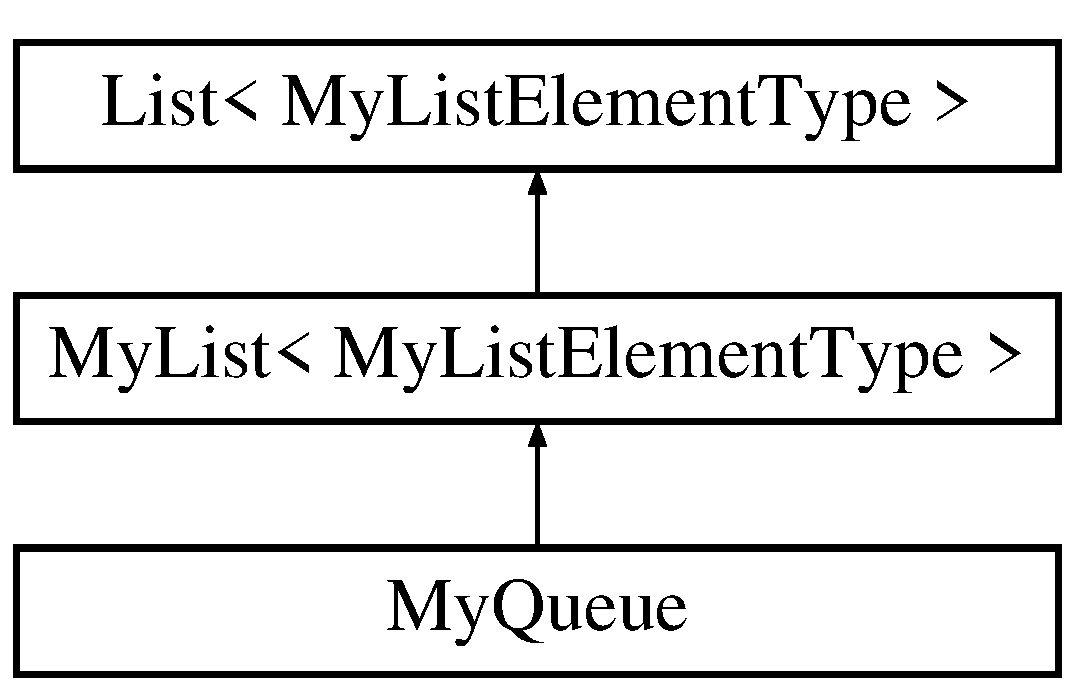
\includegraphics[height=2.000000cm]{class_my_queue}
\end{center}
\end{figure}
\subsubsection*{Metody publiczne}
\begin{DoxyCompactItemize}
\item 
void \hyperlink{class_my_queue_abc623d6dea3f8ea4c364d4e755914b89}{push} (int arg)
\item 
int \hyperlink{class_my_queue_a1515805489e2e6b4c955f8e1e62a0650}{pop} ()
\begin{DoxyCompactList}\small\item\em Wyciaga element z kolejki. \end{DoxyCompactList}\end{DoxyCompactItemize}
\subsubsection*{Dodatkowe Dziedziczone Składowe}


\subsubsection{Opis szczegółowy}


Definicja w linii \hyperlink{myqueue_8h_source_l00016}{16} pliku \hyperlink{myqueue_8h_source}{myqueue.\-h}.



\subsubsection{Dokumentacja funkcji składowych}
\hypertarget{class_my_queue_a1515805489e2e6b4c955f8e1e62a0650}{\index{My\-Queue@{My\-Queue}!pop@{pop}}
\index{pop@{pop}!MyQueue@{My\-Queue}}
\paragraph[{pop}]{\setlength{\rightskip}{0pt plus 5cm}int My\-Queue\-::pop (
\begin{DoxyParamCaption}
{}
\end{DoxyParamCaption}
)\hspace{0.3cm}{\ttfamily [inline]}}}\label{class_my_queue_a1515805489e2e6b4c955f8e1e62a0650}


Definicja w linii \hyperlink{myqueue_8h_source_l00027}{27} pliku \hyperlink{myqueue_8h_source}{myqueue.\-h}.



Odwołuje się do \hyperlink{mylist_8cpp_source_l00053}{My\-List\-::pop\-\_\-front()}.


\begin{DoxyCode}
00027                   \{
00028                 \textcolor{keywordflow}{return} \hyperlink{class_my_list_a84369accd705913f85b770770f06767a}{pop\_front}();
00029         \}
\end{DoxyCode}
\hypertarget{class_my_queue_abc623d6dea3f8ea4c364d4e755914b89}{\index{My\-Queue@{My\-Queue}!push@{push}}
\index{push@{push}!MyQueue@{My\-Queue}}
\paragraph[{push}]{\setlength{\rightskip}{0pt plus 5cm}void My\-Queue\-::push (
\begin{DoxyParamCaption}
\item[{int}]{arg}
\end{DoxyParamCaption}
)\hspace{0.3cm}{\ttfamily [inline]}}}\label{class_my_queue_abc623d6dea3f8ea4c364d4e755914b89}


Definicja w linii \hyperlink{myqueue_8h_source_l00023}{23} pliku \hyperlink{myqueue_8h_source}{myqueue.\-h}.



Odwołuje się do \hyperlink{mylist_8cpp_source_l00025}{My\-List\-::push\-\_\-back()}.


\begin{DoxyCode}
00023                            \{
00024                 \hyperlink{class_my_list_a06c2749553f559eb3d5d227e0ac07c53}{push\_back}(arg);
00025         \}
\end{DoxyCode}


Dokumentacja dla tej klasy została wygenerowana z pliku\-:\begin{DoxyCompactItemize}
\item 
\hyperlink{myqueue_8h}{myqueue.\-h}\end{DoxyCompactItemize}

\hypertarget{class_my_stack}{\subsection{Dokumentacja klasy My\-Stack}
\label{class_my_stack}\index{My\-Stack@{My\-Stack}}
}


Klasa reprezentuje stos.  




{\ttfamily \#include $<$mystack.\-h$>$}

Diagram dziedziczenia dla My\-Stack\begin{figure}[H]
\begin{center}
\leavevmode
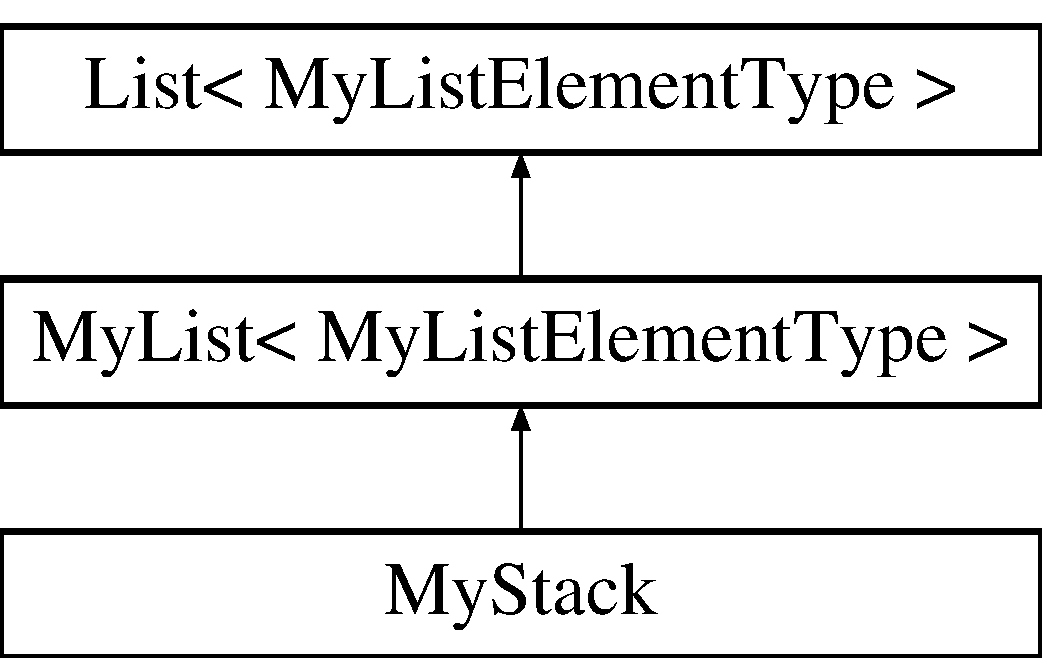
\includegraphics[height=2.000000cm]{class_my_stack}
\end{center}
\end{figure}
\subsubsection*{Metody publiczne}
\begin{DoxyCompactItemize}
\item 
void \hyperlink{class_my_stack_a481713bcbaecb7509a8903911db89331}{push} (int arg)
\item 
int \hyperlink{class_my_stack_abe5267f1fbc044957e8eb2e87fd10ca1}{pop} ()
\begin{DoxyCompactList}\small\item\em Wyciaga element ze stosu. \end{DoxyCompactList}\end{DoxyCompactItemize}
\subsubsection*{Dodatkowe Dziedziczone Składowe}


\subsubsection{Opis szczegółowy}
Stos, którego index po pushu pokazuje na miejsce nastepne(nastepne za tym elementem) 

Definicja w linii \hyperlink{mystack_8h_source_l00018}{18} pliku \hyperlink{mystack_8h_source}{mystack.\-h}.



\subsubsection{Dokumentacja funkcji składowych}
\hypertarget{class_my_stack_abe5267f1fbc044957e8eb2e87fd10ca1}{\index{My\-Stack@{My\-Stack}!pop@{pop}}
\index{pop@{pop}!MyStack@{My\-Stack}}
\paragraph[{pop}]{\setlength{\rightskip}{0pt plus 5cm}int My\-Stack\-::pop (
\begin{DoxyParamCaption}
{}
\end{DoxyParamCaption}
)\hspace{0.3cm}{\ttfamily [inline]}}}\label{class_my_stack_abe5267f1fbc044957e8eb2e87fd10ca1}


Definicja w linii \hyperlink{mystack_8h_source_l00029}{29} pliku \hyperlink{mystack_8h_source}{mystack.\-h}.



Odwołuje się do \hyperlink{mylist_8cpp_source_l00044}{My\-List\-::pop\-\_\-back()}.


\begin{DoxyCode}
00029                   \{
00030                 \textcolor{keywordflow}{return} \hyperlink{class_my_list_afc006104d8156154ad3849d0e4cc6109}{pop\_back}();
00031         \}
\end{DoxyCode}
\hypertarget{class_my_stack_a481713bcbaecb7509a8903911db89331}{\index{My\-Stack@{My\-Stack}!push@{push}}
\index{push@{push}!MyStack@{My\-Stack}}
\paragraph[{push}]{\setlength{\rightskip}{0pt plus 5cm}void My\-Stack\-::push (
\begin{DoxyParamCaption}
\item[{int}]{arg}
\end{DoxyParamCaption}
)\hspace{0.3cm}{\ttfamily [inline]}}}\label{class_my_stack_a481713bcbaecb7509a8903911db89331}


Definicja w linii \hyperlink{mystack_8h_source_l00025}{25} pliku \hyperlink{mystack_8h_source}{mystack.\-h}.



Odwołuje się do \hyperlink{mylist_8cpp_source_l00025}{My\-List\-::push\-\_\-back()}.


\begin{DoxyCode}
00025                            \{
00026                 \hyperlink{class_my_list_a06c2749553f559eb3d5d227e0ac07c53}{push\_back}(arg);
00027         \}
\end{DoxyCode}


Dokumentacja dla tej klasy została wygenerowana z pliku\-:\begin{DoxyCompactItemize}
\item 
\hyperlink{mystack_8h}{mystack.\-h}\end{DoxyCompactItemize}

\hypertarget{class_number_generator}{\subsection{Dokumentacja klasy Number\-Generator}
\label{class_number_generator}\index{Number\-Generator@{Number\-Generator}}
}


Klasa generujaca losowe liczby.  




{\ttfamily \#include $<$numbergenerator.\-h$>$}

\subsubsection*{Statyczne metody publiczne}
\begin{DoxyCompactItemize}
\item 
{\footnotesize template$<$typename Content\-Type $>$ }\\static \hyperlink{class_linked_list}{Linked\-List}$<$ Content\-Type $>$ \& \hyperlink{class_number_generator_a4a31ee39c34c77b01f19516fd5253389}{generate\-Numbers} (int range, int quantity)
\begin{DoxyCompactList}\small\item\em Generuje losowe liczby. \end{DoxyCompactList}\item 
static std\-::string $\ast$ \hyperlink{class_number_generator_afed5ae8efb72655770753790714b7643}{generate\-Strings} (int ile\-Stringow)
\begin{DoxyCompactList}\small\item\em Generuje losowe stringi. \end{DoxyCompactList}\end{DoxyCompactItemize}


\subsubsection{Opis szczegółowy}
Klasa generujaca losowe liczby na podstawie czasu maszyny na ktorym jest uruchomiona Wszystkie funkcje zapisu pliku dziedziczy z klasy Data\-Frame 

Definicja w linii \hyperlink{numbergenerator_8h_source_l00027}{27} pliku \hyperlink{numbergenerator_8h_source}{numbergenerator.\-h}.



\subsubsection{Dokumentacja funkcji składowych}
\hypertarget{class_number_generator_a4a31ee39c34c77b01f19516fd5253389}{\index{Number\-Generator@{Number\-Generator}!generate\-Numbers@{generate\-Numbers}}
\index{generate\-Numbers@{generate\-Numbers}!NumberGenerator@{Number\-Generator}}
\paragraph[{generate\-Numbers}]{\setlength{\rightskip}{0pt plus 5cm}template$<$typename Content\-Type $>$ static {\bf Linked\-List}$<$Content\-Type$>$\& Number\-Generator\-::generate\-Numbers (
\begin{DoxyParamCaption}
\item[{int}]{range, }
\item[{int}]{quantity}
\end{DoxyParamCaption}
)\hspace{0.3cm}{\ttfamily [inline]}, {\ttfamily [static]}}}\label{class_number_generator_a4a31ee39c34c77b01f19516fd5253389}


Definicja w linii \hyperlink{numbergenerator_8h_source_l00033}{33} pliku \hyperlink{numbergenerator_8h_source}{numbergenerator.\-h}.



Odwołuje się do \hyperlink{linkedlist_8h_source_l00100}{Linked\-List$<$ Content\-Type $>$\-::push\-\_\-back()}.


\begin{DoxyCode}
00034 \{
00035         \hyperlink{class_linked_list}{LinkedList<ContentType>} &myList = *\textcolor{keyword}{new} 
      \hyperlink{class_linked_list}{LinkedList<ContentType>}();
00036         time\_t randomTime = clock();
00037         \textcolor{keywordtype}{int} randomNumber;
00038         \textcolor{keywordflow}{for}(\textcolor{keywordtype}{int} i=0; i<quantity ; i++)
00039         \{
00040                 srand (randomTime = clock());
00041                 randomNumber = rand()%range;
00042                 myList.\hyperlink{class_linked_list_a719c7b47925171fd7a72a35d0a581619}{push\_back}(randomNumber);
00043                 randomTime = clock();
00044         \}
00045         \textcolor{keywordflow}{return} myList;
00046 \}
\end{DoxyCode}
\hypertarget{class_number_generator_afed5ae8efb72655770753790714b7643}{\index{Number\-Generator@{Number\-Generator}!generate\-Strings@{generate\-Strings}}
\index{generate\-Strings@{generate\-Strings}!NumberGenerator@{Number\-Generator}}
\paragraph[{generate\-Strings}]{\setlength{\rightskip}{0pt plus 5cm}static std\-::string$\ast$ Number\-Generator\-::generate\-Strings (
\begin{DoxyParamCaption}
\item[{int}]{ile\-Stringow}
\end{DoxyParamCaption}
)\hspace{0.3cm}{\ttfamily [static]}}}\label{class_number_generator_afed5ae8efb72655770753790714b7643}

\begin{DoxyParams}{Parametry}
{\em ile\-Stringow} & Ilosc stringow do stworzenia Generuje losowe stringi na podstawie czasu maszyny \\
\hline
\end{DoxyParams}


Dokumentacja dla tej klasy została wygenerowana z pliku\-:\begin{DoxyCompactItemize}
\item 
\hyperlink{numbergenerator_8h}{numbergenerator.\-h}\end{DoxyCompactItemize}

\input{class_stack_on_array}
\section{Dokumentacja plików}
\input{dataframe_8cpp}
\input{dataframe_8cpp_source}
\input{dataframe_8h}
\input{dataframe_8h_source}
\hypertarget{dictionary_8cpp}{\subsection{Dokumentacja pliku dictionary.\-cpp}
\label{dictionary_8cpp}\index{dictionary.\-cpp@{dictionary.\-cpp}}
}
{\ttfamily \#include \char`\"{}dictionary.\-h\char`\"{}}\\*

\hypertarget{dictionary_8cpp}{\subsection{dictionary.\-cpp}
\label{dictionary_8cpp}\index{dictionary.\-cpp@{dictionary.\-cpp}}
}

\begin{DoxyCode}
00001 \textcolor{comment}{/*}
00002 \textcolor{comment}{ * dictionary.cpp}
00003 \textcolor{comment}{ *}
00004 \textcolor{comment}{ *  Created on: Apr 14, 2015}
00005 \textcolor{comment}{ *      Author: serek8}
00006 \textcolor{comment}{ */}
00007 
00008 \textcolor{preprocessor}{#include "\hyperlink{dictionary_8h}{dictionary.h}"}
00009 
00010 
\hypertarget{dictionary_8cpp_source_l00011}{}\hyperlink{class_dictionary_a5a82ede9a412aa8a9b7bee9b2a423427}{00011}         \textcolor{keywordtype}{int} &\hyperlink{class_dictionary_a5a82ede9a412aa8a9b7bee9b2a423427}{Dictionary::operator[]}(\textcolor{keywordtype}{string} str)
00012         \{
00013                 \hyperlink{class_my_list}{MyList} tmpList;
00014                 \hyperlink{class_my_list_1_1_my_list_element}{MyList::MyListElement} tmpListElement;
00015                 \textcolor{keywordtype}{int} \textcolor{keywordtype}{id} = \hyperlink{class_dictionary_a53981ac20e3ab2b7544d6f6f3111cdf4}{str2int}(str);
00016                 \textcolor{comment}{// jezeli sa elementy na liscie}
00017                 \textcolor{comment}{//std::cerr<<"\(\backslash\)nSize listy na wejsciu do funkcji []: "<<kolumnaList[id].size();}
00018                 \textcolor{keywordflow}{while}(\hyperlink{class_dictionary_a36adbe694dbbdcbd577d9e8486bdf40a}{kolumnaList}[\textcolor{keywordtype}{id}].size())
00019                 \{
00020                 \textcolor{comment}{//std::cerr<<"\(\backslash\)nSize listy na wejsciu do while I []: "<<kolumnaList[id].size();}
00021                 \textcolor{comment}{//std::cerr<<"\(\backslash\)nhash id:"<<id;}
00022                 tmpListElement = \hyperlink{class_dictionary_a36adbe694dbbdcbd577d9e8486bdf40a}{kolumnaList}[id].\hyperlink{class_my_list_a84369accd705913f85b770770f06767a}{pop\_front}();
00023                 \textcolor{comment}{//std::cerr<<"\(\backslash\)nWyjalem klucz z liczba: "<<tmpListElement.number;}
00024                         \textcolor{keywordflow}{if}( !(tmpListElement.\hyperlink{class_my_list_1_1_my_list_element_af610aeae835150be1a12d538e67a579c}{nazwa}.compare(str)) ) \textcolor{comment}{// znalazlem taki sam klucz w
       slowniku}
00025                                 \{
00026                                 \textcolor{comment}{//std::cerr<<"\(\backslash\)nZnalazlem takie same klucze";}
00027                                         \textcolor{keywordflow}{while}(tmpList.\hyperlink{class_my_list_a6d21c8bfbd9cd31efdba81ba488f43f2}{size}())
00028                                         \{
00029                                                 \hyperlink{class_dictionary_a36adbe694dbbdcbd577d9e8486bdf40a}{kolumnaList}[id].
      \hyperlink{class_my_list_ac703cd9be1c465722e683dbdcececa6b}{push\_front}(tmpList.\hyperlink{class_my_list_afc006104d8156154ad3849d0e4cc6109}{pop\_back}());
00030                                         \}
00031                                         \hyperlink{class_dictionary_a36adbe694dbbdcbd577d9e8486bdf40a}{kolumnaList}[id].\hyperlink{class_my_list_ac703cd9be1c465722e683dbdcececa6b}{push\_front}(tmpListElement);
00032                                         \textcolor{keywordflow}{return} (\hyperlink{class_dictionary_a36adbe694dbbdcbd577d9e8486bdf40a}{kolumnaList}[\textcolor{keywordtype}{id}]).show\_front().number;
00033                                 \}
00034                         \textcolor{keywordflow}{else}
00035                         \{
00036                                 tmpList.\hyperlink{class_my_list_ac703cd9be1c465722e683dbdcececa6b}{push\_front}(tmpListElement);
00037                         \}
00038                 \}
00039                 \textcolor{comment}{//Czyli nie znalazlem takiego elementu, to go tworze}
00040                 tmpListElement.\hyperlink{class_my_list_1_1_my_list_element_acd6dbb6a8791f034f94678d46395b366}{number}=0;
00041                 tmpListElement.\hyperlink{class_my_list_1_1_my_list_element_af610aeae835150be1a12d538e67a579c}{nazwa}=str;
00042                 tmpList.\hyperlink{class_my_list_ac703cd9be1c465722e683dbdcececa6b}{push\_front}(tmpListElement);
00043                 \hyperlink{class_dictionary_a36adbe694dbbdcbd577d9e8486bdf40a}{kolumnaList}[id] = tmpList;
00044                 \textcolor{comment}{//std::cerr<<"\(\backslash\)nZapisalem nowy element: "<<kolumnaList[id].show\_front().number;}
00045                 \textcolor{keywordflow}{return} \hyperlink{class_dictionary_a36adbe694dbbdcbd577d9e8486bdf40a}{kolumnaList}[id].\hyperlink{class_my_list_a9d7990c6a8b96d4c0d267fe46582fd6b}{show\_front}().\hyperlink{class_my_list_1_1_my_list_element_acd6dbb6a8791f034f94678d46395b366}{number};
00046         \}
00047 
00048 
00049 
00050 
\hypertarget{dictionary_8cpp_source_l00051}{}\hyperlink{class_dictionary_a53981ac20e3ab2b7544d6f6f3111cdf4}{00051}         \textcolor{keywordtype}{int} \hyperlink{class_dictionary_a53981ac20e3ab2b7544d6f6f3111cdf4}{Dictionary::str2int}(\textcolor{keywordtype}{string} str)\{
00052                 \textcolor{keywordtype}{int} hash=0;
00053                 \textcolor{keywordflow}{for}(\textcolor{keywordtype}{unsigned} \textcolor{keywordtype}{int} i=0; ( i<\hyperlink{dictionary_8h_a562499e66e3ed9cc37111ac1ddafa1eb}{LICZBA\_ZNAKOW\_DO\_HASHU} && i<str.size() );i+
      +)
00054                         hash += (\textcolor{keywordtype}{int})str[i];
00055                 \textcolor{comment}{//std::cout<<"\(\backslash\)nHash:"<<hash;}
00056                 \textcolor{keywordflow}{return} hash;
00057         \}
00058 
00059 
\end{DoxyCode}

\hypertarget{dictionary_8h}{\subsection{Dokumentacja pliku dictionary.\-h}
\label{dictionary_8h}\index{dictionary.\-h@{dictionary.\-h}}
}
{\ttfamily \#include $<$string$>$}\\*
{\ttfamily \#include $<$iostream$>$}\\*
{\ttfamily \#include \char`\"{}mylist.\-h\char`\"{}}\\*
{\ttfamily \#include \char`\"{}numbergenerator.\-h\char`\"{}}\\*
\subsubsection*{Komponenty}
\begin{DoxyCompactItemize}
\item 
class \hyperlink{class_dictionary}{Dictionary}
\begin{DoxyCompactList}\small\item\em Klasa tworzy tablicy asocjacyjną -\/ słownik. \end{DoxyCompactList}\end{DoxyCompactItemize}
\subsubsection*{Definicje}
\begin{DoxyCompactItemize}
\item 
\#define \hyperlink{dictionary_8h_a562499e66e3ed9cc37111ac1ddafa1eb}{L\-I\-C\-Z\-B\-A\-\_\-\-Z\-N\-A\-K\-O\-W\-\_\-\-D\-O\-\_\-\-H\-A\-S\-H\-U}~3
\end{DoxyCompactItemize}


\subsubsection{Dokumentacja definicji}
\hypertarget{dictionary_8h_a562499e66e3ed9cc37111ac1ddafa1eb}{\index{dictionary.\-h@{dictionary.\-h}!L\-I\-C\-Z\-B\-A\-\_\-\-Z\-N\-A\-K\-O\-W\-\_\-\-D\-O\-\_\-\-H\-A\-S\-H\-U@{L\-I\-C\-Z\-B\-A\-\_\-\-Z\-N\-A\-K\-O\-W\-\_\-\-D\-O\-\_\-\-H\-A\-S\-H\-U}}
\index{L\-I\-C\-Z\-B\-A\-\_\-\-Z\-N\-A\-K\-O\-W\-\_\-\-D\-O\-\_\-\-H\-A\-S\-H\-U@{L\-I\-C\-Z\-B\-A\-\_\-\-Z\-N\-A\-K\-O\-W\-\_\-\-D\-O\-\_\-\-H\-A\-S\-H\-U}!dictionary.h@{dictionary.\-h}}
\paragraph[{L\-I\-C\-Z\-B\-A\-\_\-\-Z\-N\-A\-K\-O\-W\-\_\-\-D\-O\-\_\-\-H\-A\-S\-H\-U}]{\setlength{\rightskip}{0pt plus 5cm}\#define L\-I\-C\-Z\-B\-A\-\_\-\-Z\-N\-A\-K\-O\-W\-\_\-\-D\-O\-\_\-\-H\-A\-S\-H\-U~3}}\label{dictionary_8h_a562499e66e3ed9cc37111ac1ddafa1eb}


Definicja w linii \hyperlink{dictionary_8h_source_l00010}{10} pliku \hyperlink{dictionary_8h_source}{dictionary.\-h}.



Odwołania w \hyperlink{dictionary_8h_source_l00037}{Dictionary\-::\-Dictionary()}, \hyperlink{main_8cpp_source_l00018}{main()} i \hyperlink{dictionary_8cpp_source_l00051}{Dictionary\-::str2int()}.


\hypertarget{dictionary_8h}{\subsection{dictionary.\-h}
\label{dictionary_8h}\index{dictionary.\-h@{dictionary.\-h}}
}

\begin{DoxyCode}
00001 \textcolor{comment}{/*}
00002 \textcolor{comment}{ * dictionary.h}
00003 \textcolor{comment}{ *}
00004 \textcolor{comment}{ *  Created on: Apr 9, 2015}
00005 \textcolor{comment}{ *      Author: serek8}
00006 \textcolor{comment}{ */}
00007 
00008 \textcolor{preprocessor}{#ifndef DICTIONARY\_H\_}
00009 \textcolor{preprocessor}{}\textcolor{preprocessor}{#define DICTIONARY\_H\_}
\hypertarget{dictionary_8h_source_l00010}{}\hyperlink{dictionary_8h_a562499e66e3ed9cc37111ac1ddafa1eb}{00010} \textcolor{preprocessor}{}\textcolor{preprocessor}{#define LICZBA\_ZNAKOW\_DO\_HASHU 3}
00011 \textcolor{preprocessor}{}
00012 \textcolor{preprocessor}{#include <string>}
00013 \textcolor{preprocessor}{#include <iostream>}
00014 \textcolor{preprocessor}{#include "\hyperlink{mylist_8h}{mylist.h}"}
00015 \textcolor{preprocessor}{#include "\hyperlink{numbergenerator_8h}{numbergenerator.h}"}
00016 \textcolor{keyword}{using namespace }std;
00017 
\hypertarget{dictionary_8h_source_l00025}{}\hyperlink{class_dictionary}{00025} \textcolor{keyword}{class }\hyperlink{class_dictionary}{Dictionary}
00026 \{
\hypertarget{dictionary_8h_source_l00030}{}\hyperlink{class_dictionary_a36adbe694dbbdcbd577d9e8486bdf40a}{00030}         \hyperlink{class_my_list}{MyList} *\hyperlink{class_dictionary_a36adbe694dbbdcbd577d9e8486bdf40a}{kolumnaList};
00031 
00032 \textcolor{keyword}{public}:
\hypertarget{dictionary_8h_source_l00037}{}\hyperlink{class_dictionary_aee8d612bc9d323c38faba045ba384b8b}{00037}         \hyperlink{class_dictionary_aee8d612bc9d323c38faba045ba384b8b}{Dictionary}() \{        kolumnaList = \textcolor{keyword}{new} \hyperlink{class_my_list}{MyList}[ 
      \hyperlink{dictionary_8h_a562499e66e3ed9cc37111ac1ddafa1eb}{LICZBA\_ZNAKOW\_DO\_HASHU} * \hyperlink{numbergenerator_8h_ad234b171c744b5f476c1685da37bb7ca}{MAX\_HEX\_ASCII\_KOD}+1]; \}
00038 
00043         \textcolor{keyword}{static} \textcolor{keywordtype}{int} str2int(\textcolor{keywordtype}{string} str);
00048         \textcolor{keyword}{static} \textcolor{keywordtype}{int} str2intAll(\textcolor{keywordtype}{string} str);
00056         \textcolor{keywordtype}{int} &operator[](\textcolor{keywordtype}{string} str);
00057 \};
00058 
00059 
00060 
00061 
00062 
00063 
00064 \textcolor{preprocessor}{#endif }\textcolor{comment}{/* DICTIONARY\_H\_ */}\textcolor{preprocessor}{}
\end{DoxyCode}

\hypertarget{hashowanie_8h}{\subsection{Dokumentacja pliku hashowanie.\-h}
\label{hashowanie_8h}\index{hashowanie.\-h@{hashowanie.\-h}}
}
{\ttfamily \#include $<$string$>$}\\*
{\ttfamily \#include $<$iostream$>$}\\*
\subsubsection*{Komponenty}
\begin{DoxyCompactItemize}
\item 
class \hyperlink{class_hashowanie}{Hashowanie}
\end{DoxyCompactItemize}

\hypertarget{hashowanie_8h}{\subsection{hashowanie.\-h}
\label{hashowanie_8h}\index{hashowanie.\-h@{hashowanie.\-h}}
}

\begin{DoxyCode}
00001 \textcolor{comment}{/*}
00002 \textcolor{comment}{ * hashowanie.h}
00003 \textcolor{comment}{ *}
00004 \textcolor{comment}{ *  Created on: Apr 9, 2015}
00005 \textcolor{comment}{ *      Author: serek8}
00006 \textcolor{comment}{ */}
00007 
00008 \textcolor{preprocessor}{#ifndef HASHOWANIE\_H\_}
00009 \textcolor{preprocessor}{}\textcolor{preprocessor}{#define HASHOWANIE\_H\_}
00010 \textcolor{preprocessor}{}\textcolor{preprocessor}{#include <string>}
00011 \textcolor{preprocessor}{#include <iostream>}
00012 \textcolor{keyword}{using namespace }std;
\hypertarget{hashowanie_8h_source_l00013}{}\hyperlink{class_hashowanie}{00013} \textcolor{keyword}{class }\hyperlink{class_hashowanie}{Hashowanie}
00014 \{
00015 \textcolor{keyword}{public}:
\hypertarget{hashowanie_8h_source_l00016}{}\hyperlink{class_hashowanie_a110b055bf2be74d6588c9ff20baddbbb}{00016}         \textcolor{keyword}{static} \textcolor{keywordtype}{int} \hyperlink{class_hashowanie_a110b055bf2be74d6588c9ff20baddbbb}{str2int}(\textcolor{keyword}{const} \textcolor{keywordtype}{char}* str)\{
00017                 \textcolor{keywordtype}{int} hash;
00018                 hash = (int)str[0]+(\textcolor{keywordtype}{int})str[1]+(int)str[2];
00019                 std::cout<<\textcolor{stringliteral}{"\(\backslash\)nHash:"}<<hash;
00020                 \textcolor{keywordflow}{return} hash;
00021         \}
00022 
00023 
00024 
00025 \};
00026 
00027 
00028 
00029 
00030 
00031 \textcolor{preprocessor}{#endif }\textcolor{comment}{/* HASHOWANIE\_H\_ */}\textcolor{preprocessor}{}
\end{DoxyCode}

\hypertarget{main_8cpp}{\subsection{Dokumentacja pliku main.\-cpp}
\label{main_8cpp}\index{main.\-cpp@{main.\-cpp}}
}
{\ttfamily \#include $<$iostream$>$}\\*
{\ttfamily \#include $<$unistd.\-h$>$}\\*
{\ttfamily \#include \char`\"{}numbergenerator.\-h\char`\"{}}\\*
{\ttfamily \#include \char`\"{}observableavltree.\-h\char`\"{}}\\*
{\ttfamily \#include \char`\"{}mybenchmark.\-h\char`\"{}}\\*
{\ttfamily \#include \char`\"{}mylist.\-h\char`\"{}}\\*
\subsubsection*{Definicje}
\begin{DoxyCompactItemize}
\item 
\#define \hyperlink{main_8cpp_adfa2ae8b78bba187e8a03a23e9b2617d}{I\-L\-E\-\_\-\-W\-Y\-R\-A\-Z\-O\-W\-\_\-\-D\-O\-\_\-\-W\-S\-T\-A\-W\-I\-E\-N\-I\-A}~100
\end{DoxyCompactItemize}
\subsubsection*{Funkcje}
\begin{DoxyCompactItemize}
\item 
int \hyperlink{main_8cpp_a0ddf1224851353fc92bfbff6f499fa97}{main} (int argc, char $\ast$argv\mbox{[}$\,$\mbox{]})
\end{DoxyCompactItemize}


\subsubsection{Dokumentacja definicji}
\hypertarget{main_8cpp_adfa2ae8b78bba187e8a03a23e9b2617d}{\index{main.\-cpp@{main.\-cpp}!I\-L\-E\-\_\-\-W\-Y\-R\-A\-Z\-O\-W\-\_\-\-D\-O\-\_\-\-W\-S\-T\-A\-W\-I\-E\-N\-I\-A@{I\-L\-E\-\_\-\-W\-Y\-R\-A\-Z\-O\-W\-\_\-\-D\-O\-\_\-\-W\-S\-T\-A\-W\-I\-E\-N\-I\-A}}
\index{I\-L\-E\-\_\-\-W\-Y\-R\-A\-Z\-O\-W\-\_\-\-D\-O\-\_\-\-W\-S\-T\-A\-W\-I\-E\-N\-I\-A@{I\-L\-E\-\_\-\-W\-Y\-R\-A\-Z\-O\-W\-\_\-\-D\-O\-\_\-\-W\-S\-T\-A\-W\-I\-E\-N\-I\-A}!main.cpp@{main.\-cpp}}
\paragraph[{I\-L\-E\-\_\-\-W\-Y\-R\-A\-Z\-O\-W\-\_\-\-D\-O\-\_\-\-W\-S\-T\-A\-W\-I\-E\-N\-I\-A}]{\setlength{\rightskip}{0pt plus 5cm}\#define I\-L\-E\-\_\-\-W\-Y\-R\-A\-Z\-O\-W\-\_\-\-D\-O\-\_\-\-W\-S\-T\-A\-W\-I\-E\-N\-I\-A~100}}\label{main_8cpp_adfa2ae8b78bba187e8a03a23e9b2617d}


Definicja w linii \hyperlink{main_8cpp_source_l00015}{15} pliku \hyperlink{main_8cpp_source}{main.\-cpp}.



Odwołania w \hyperlink{main_8cpp_source_l00017}{main()}.



\subsubsection{Dokumentacja funkcji}
\hypertarget{main_8cpp_a0ddf1224851353fc92bfbff6f499fa97}{\index{main.\-cpp@{main.\-cpp}!main@{main}}
\index{main@{main}!main.cpp@{main.\-cpp}}
\paragraph[{main}]{\setlength{\rightskip}{0pt plus 5cm}int main (
\begin{DoxyParamCaption}
\item[{int}]{argc, }
\item[{char $\ast$}]{argv\mbox{[}$\,$\mbox{]}}
\end{DoxyParamCaption}
)}}\label{main_8cpp_a0ddf1224851353fc92bfbff6f499fa97}


Definicja w linii \hyperlink{main_8cpp_source_l00017}{17} pliku \hyperlink{main_8cpp_source}{main.\-cpp}.



Odwołuje się do \hyperlink{main_8cpp_source_l00015}{I\-L\-E\-\_\-\-W\-Y\-R\-A\-Z\-O\-W\-\_\-\-D\-O\-\_\-\-W\-S\-T\-A\-W\-I\-E\-N\-I\-A} i \hyperlink{mylist_8h_source_l00066}{My\-List$<$ My\-List\-Element\-Type $>$\-::size()}.


\begin{DoxyCode}
00018 \{
00019         \hyperlink{class_my_list}{MyList<int>} lista;
00020 
00021 
00022         lista = NumberGenerator::generateNumbers<int>(100, 
      \hyperlink{main_8cpp_adfa2ae8b78bba187e8a03a23e9b2617d}{ILE\_WYRAZOW\_DO\_WSTAWIENIA});
00023         \hyperlink{class_observable_a_v_l_tree}{ObservableAVLTree<int>} tree;
00024         \hyperlink{class_my_benchmark_observer}{MyBenchmarkObserver} *o1 = \textcolor{keyword}{new} \hyperlink{class_my_benchmark_observer}{MyBenchmarkObserver}();
00025         tree.add(o1);
00026 
00027         \textcolor{keywordflow}{for}(\textcolor{keywordtype}{int} i=0; i<lista.\hyperlink{class_my_list_a267f669859ef3541333082cad6b28ab7}{size}(); i++)
00028         \{
00029                 tree.insert(lista[i].content);
00030         \}
00031         std::cout<<std::endl;
00032         \textcolor{keywordflow}{return} 0;
00033 \}
\end{DoxyCode}

\hypertarget{main_8cpp}{\subsection{main.\-cpp}
\label{main_8cpp}\index{main.\-cpp@{main.\-cpp}}
}

\begin{DoxyCode}
00001 \textcolor{comment}{/*}
00002 \textcolor{comment}{ * main.cpp}
00003 \textcolor{comment}{ *}
00004 \textcolor{comment}{ *  Created on: Mar 6, 2015}
00005 \textcolor{comment}{ *      Author: serek8}
00006 \textcolor{comment}{ */}
00008 \textcolor{preprocessor}{#include <iostream>}
00009 \textcolor{preprocessor}{#include <unistd.h>}
00010 \textcolor{preprocessor}{#include "\hyperlink{numbergenerator_8h}{numbergenerator.h}"}
00011 \textcolor{preprocessor}{#include "\hyperlink{dataframe_8h}{dataframe.h}"}
00012 \textcolor{preprocessor}{#include "\hyperlink{hashowanie_8h}{hashowanie.h}"}
00013 \textcolor{preprocessor}{#include "\hyperlink{mylist_8h}{mylist.h}"}
00014 \textcolor{preprocessor}{#include "\hyperlink{mybenchmark_8h}{mybenchmark.h}"}
00015 \textcolor{preprocessor}{#include "\hyperlink{dictionary_8h}{dictionary.h}"}
00016 \textcolor{preprocessor}{#include <string>}
00017 
\hypertarget{main_8cpp_source_l00018}{}\hyperlink{main_8cpp_a0ddf1224851353fc92bfbff6f499fa97}{00018} \textcolor{keywordtype}{int} \hyperlink{main_8cpp_a0ddf1224851353fc92bfbff6f499fa97}{main}(\textcolor{keywordtype}{int} argc, \textcolor{keywordtype}{char} *argv[])
00019 \{
00020         \hyperlink{class_data_frame}{DataFrame} podstawoweInfoIO;
00021 
00022         \textcolor{keywordtype}{int} opt;        
00023         \textcolor{keywordtype}{bool} isSetNumberGenerator=\textcolor{keyword}{false}; 
00024         \textcolor{comment}{//bool isTest=false;}
00025 
00026         \textcolor{keywordflow}{while} ((opt = getopt(argc, argv, \textcolor{stringliteral}{"n:o:i:gx"})) != -1) \{
00027                 \textcolor{keywordflow}{switch}(opt)\{
00028                 \textcolor{keywordflow}{case} \textcolor{charliteral}{'n'}:       \textcolor{comment}{// ilosc liczb do przetworzenia}
00029                         podstawoweInfoIO.\hyperlink{class_data_frame_aa5d1905c6910cad07ab5189bd34b13ab}{sizeOfTable} = atoi(optarg);
00030                         \textcolor{keywordflow}{break};
00031 
00032 
00033                 \textcolor{keywordflow}{case} \textcolor{charliteral}{'o'}:
00034                         podstawoweInfoIO.\hyperlink{class_data_frame_a824a73f019aec71281837abafd95a510}{outputFileName} = optarg;
00035                         \textcolor{keywordflow}{break};
00036 
00037                 \textcolor{keywordflow}{case} \textcolor{charliteral}{'i'}:
00038                         podstawoweInfoIO.\hyperlink{class_data_frame_a90041bfdf474b0d7ce39bc3dbbb55aa9}{inputFileName}=optarg;
00039                         \textcolor{keywordflow}{break};
00040 
00041                 \textcolor{keywordflow}{case} \textcolor{charliteral}{'g'}:       \textcolor{comment}{// wlacza generator liczb, po zakonczeniu generowania konczy program}
00042                         isSetNumberGenerator=\textcolor{keyword}{true};
00043                         \textcolor{keywordflow}{break};
00044 
00045 
00046                 \textcolor{keywordflow}{case} \textcolor{charliteral}{'?'}:
00047                 \textcolor{keywordflow}{default}:
00048                         std::cout<<\textcolor{stringliteral}{"\(\backslash\)nPodano zly argument"};
00049                         \textcolor{keywordflow}{return} -1;
00050                 \}
00051         \}
00052 
00053 
00054         \textcolor{comment}{// na potrzeby slownika wlaczam generowanie automatyczne}
00055         isSetNumberGenerator = \textcolor{keyword}{true};
00056         \textcolor{keywordflow}{if}(isSetNumberGenerator) \{
00057                 \hyperlink{class_number_generator}{NumberGenerator} generator;
00058                 std::cout<<\textcolor{stringliteral}{"\(\backslash\)n+ - - - - Tworzenie tablicy i generacja losowych liczb - - - +\(\backslash\)n"};
00059                 generator= podstawoweInfoIO;
00060                 \hyperlink{class_my_benchmark_a802577db97fd440a3920add30c35a676}{MyBenchmark::timerStart}();
00061                         generator.\hyperlink{class_number_generator_a511673bb245d14a048702558d12deb63}{generateNumbers}();
00062                 std::cout<<\textcolor{stringliteral}{"Generuje losowe liczby:"}<<\hyperlink{class_my_benchmark_a7e3fa28fab999435bd4c51d915e42809}{MyBenchmark::timerStop}()<<\textcolor{charliteral}{'\(\backslash\)n'};
00063                 podstawoweInfoIO = generator;
00064                 podstawoweInfoIO.\hyperlink{class_data_frame_a03cc3ac606fdb8a2dbcaea5d429cf208}{saveDataToFile}();
00065         \}
00066 
00067         \hyperlink{class_dictionary}{Dictionary} dict;
00068         std::cout<<\textcolor{stringliteral}{"\(\backslash\)nHashuje pierwsze "}<<\hyperlink{dictionary_8h_a562499e66e3ed9cc37111ac1ddafa1eb}{LICZBA\_ZNAKOW\_DO\_HASHU}<< \textcolor{stringliteral}{" znaki."};
00069         std::string *str = \hyperlink{class_number_generator_af434d1cd0b338d22b11b24fbd2e14dce}{NumberGenerator::generateStrings}(
      podstawoweInfoIO.\hyperlink{class_data_frame_aa5d1905c6910cad07ab5189bd34b13ab}{sizeOfTable});
00070         \hyperlink{class_my_benchmark_a802577db97fd440a3920add30c35a676}{MyBenchmark::timerStart}();
00071                 \textcolor{keywordflow}{for}(\textcolor{keywordtype}{unsigned} \textcolor{keywordtype}{int} i=0; i<podstawoweInfoIO.\hyperlink{class_data_frame_aa5d1905c6910cad07ab5189bd34b13ab}{sizeOfTable}; i++)
00072                 \{
00073                         dict[str[i]] = podstawoweInfoIO.\hyperlink{class_data_frame_a8edc4ce524483e2e5069067267ccdcbf}{tableOfData}[i];
00074                 \}
00075         std::cout<<\textcolor{stringliteral}{"\(\backslash\)nCzas alokowania slownika:"}<<\hyperlink{class_my_benchmark_a7e3fa28fab999435bd4c51d915e42809}{MyBenchmark::timerStop}()<<\textcolor{charliteral}{'\(\backslash\)n'};
00076 
00077         std::cout<<std::endl;
00078         \textcolor{keywordflow}{return} 0;
00079 \}
\end{DoxyCode}

\input{multiplybytwo_8cpp}
\input{multiplybytwo_8cpp_source}
\input{multiplybytwo_8h}
\input{multiplybytwo_8h_source}
\input{mybenchmark_8cpp}
\hypertarget{mybenchmark_8cpp}{\subsection{mybenchmark.\-cpp}
\label{mybenchmark_8cpp}\index{mybenchmark.\-cpp@{mybenchmark.\-cpp}}
}

\begin{DoxyCode}
00001 \textcolor{comment}{/*}
00002 \textcolor{comment}{ * mybenchmark.cpp}
00003 \textcolor{comment}{ *}
00004 \textcolor{comment}{ *  Created on: Mar 6, 2015}
00005 \textcolor{comment}{ *      Author: serek8}
00006 \textcolor{comment}{ */}
00009 \textcolor{preprocessor}{#include "\hyperlink{mybenchmark_8h}{mybenchmark.h}"}
00010 
00011 
\hypertarget{mybenchmark_8cpp_source_l00012}{}\hyperlink{class_my_benchmark_a802577db97fd440a3920add30c35a676}{00012} \textcolor{keywordtype}{void} \hyperlink{class_my_benchmark_a802577db97fd440a3920add30c35a676}{MyBenchmark :: timerStart}()
00013 \{
00014         \hyperlink{class_my_benchmark_aeca64d5b265e357ef879bf982dd4bb00}{MyBenchmark::timerValueStatic} = (( (double)clock() ) /CLOCKS\_PER\_SEC);
00015 \}
00016 
\hypertarget{mybenchmark_8cpp_source_l00017}{}\hyperlink{class_my_benchmark_a7e3fa28fab999435bd4c51d915e42809}{00017} \textcolor{keywordtype}{double} \hyperlink{class_my_benchmark_a7e3fa28fab999435bd4c51d915e42809}{MyBenchmark :: timerStop}()
00018 \{
00019         \textcolor{keywordflow}{return} (( (\textcolor{keywordtype}{double})clock() ) /CLOCKS\_PER\_SEC) - 
      \hyperlink{class_my_benchmark_aeca64d5b265e357ef879bf982dd4bb00}{MyBenchmark::timerValueStatic};
00020 \}
00021 
\hypertarget{mybenchmark_8cpp_source_l00022}{}\hyperlink{class_my_benchmark_a94dd5cae9837db8f84eae09498b1039a}{00022} \textcolor{keywordtype}{double} \hyperlink{class_my_benchmark_a94dd5cae9837db8f84eae09498b1039a}{MyBenchmark :: timerStopAndSaveToFile}()
00023 \{
00024         \textcolor{keywordtype}{double} x= \hyperlink{class_my_benchmark_a7e3fa28fab999435bd4c51d915e42809}{timerStop}();
00025                         \hyperlink{class_my_benchmark_a45b39f704800f8403789ff5c9bbb486b}{streamToFile}<<x;
00026                         \textcolor{keywordflow}{return} x;
00027 \}
\hypertarget{mybenchmark_8cpp_source_l00028}{}\hyperlink{class_my_benchmark_ad2892ee2549d320f9e19060f444cb0d6}{00028} \textcolor{keywordtype}{void} \hyperlink{class_my_benchmark_ad2892ee2549d320f9e19060f444cb0d6}{MyBenchmark :: tab}()
00029 \{
00030         \hyperlink{class_my_benchmark_a45b39f704800f8403789ff5c9bbb486b}{streamToFile}<<\textcolor{stringliteral}{" "};
00031 
00032 \}
\hypertarget{mybenchmark_8cpp_source_l00033}{}\hyperlink{class_my_benchmark_a29b612fc55d1da88d44a6899bc89d312}{00033} \textcolor{keywordtype}{void} \hyperlink{class_my_benchmark_a29b612fc55d1da88d44a6899bc89d312}{MyBenchmark :: newL}()
00034 \{
00035         \hyperlink{class_my_benchmark_a45b39f704800f8403789ff5c9bbb486b}{streamToFile}<<\textcolor{stringliteral}{"\(\backslash\)n"};
00036 
00037 \}
\end{DoxyCode}

\hypertarget{mybenchmark_8h}{\subsection{Dokumentacja pliku mybenchmark.\-h}
\label{mybenchmark_8h}\index{mybenchmark.\-h@{mybenchmark.\-h}}
}
{\ttfamily \#include $<$ctime$>$}\\*
{\ttfamily \#include \char`\"{}observer.\-h\char`\"{}}\\*
{\ttfamily \#include $<$iostream$>$}\\*
{\ttfamily \#include $<$fstream$>$}\\*
\subsubsection*{Komponenty}
\begin{DoxyCompactItemize}
\item 
class \hyperlink{class_my_benchmark}{My\-Benchmark}
\begin{DoxyCompactList}\small\item\em Klasa bazowa/interface do testowania algorytmu. \end{DoxyCompactList}\item 
class \hyperlink{class_my_benchmark_observer}{My\-Benchmark\-Observer}
\end{DoxyCompactItemize}

\hypertarget{mybenchmark_8h}{\subsection{mybenchmark.\-h}
\label{mybenchmark_8h}\index{mybenchmark.\-h@{mybenchmark.\-h}}
}

\begin{DoxyCode}
00001 \textcolor{comment}{/*}
00002 \textcolor{comment}{ * mybenchmark.h}
00003 \textcolor{comment}{ *}
00004 \textcolor{comment}{ *  Created on: Mar 6, 2015}
00005 \textcolor{comment}{ *      Author: serek8}
00006 \textcolor{comment}{ */}
00008 \textcolor{preprocessor}{#ifndef MYBENCHMARK\_H\_}
00009 \textcolor{preprocessor}{}\textcolor{preprocessor}{#define MYBENCHMARK\_H\_}
00010 \textcolor{preprocessor}{}
00011 \textcolor{preprocessor}{#include <ctime>}
00012 \textcolor{preprocessor}{#include "\hyperlink{observer_8h}{observer.h}"}
00013 \textcolor{preprocessor}{#include <iostream>}
\hypertarget{mybenchmark_8h_source_l00020}{}\hyperlink{class_my_benchmark}{00020} \textcolor{keyword}{class }\hyperlink{class_my_benchmark}{MyBenchmark}
00021 \{
00022 \textcolor{keyword}{public}:
00023 
\hypertarget{mybenchmark_8h_source_l00025}{}\hyperlink{class_my_benchmark_a1cdab837ead670bd438f249ee82c8eff}{00025}         \textcolor{keywordtype}{double} \hyperlink{class_my_benchmark_a1cdab837ead670bd438f249ee82c8eff}{timerValue};
00026 
\hypertarget{mybenchmark_8h_source_l00027}{}\hyperlink{class_my_benchmark_a7f3739e8b61939627c0f63948a9975ca}{00027}         \hyperlink{class_my_benchmark_a7f3739e8b61939627c0f63948a9975ca}{MyBenchmark}()
00028         \{
00029                 \hyperlink{class_my_benchmark_a1cdab837ead670bd438f249ee82c8eff}{timerValue} = 0;
00030         \}
00031 
00033         \textcolor{keywordtype}{void} \hyperlink{class_my_benchmark_a802577db97fd440a3920add30c35a676}{timerStart}();
00034 
00039         \textcolor{keywordtype}{double} \hyperlink{class_my_benchmark_a7e3fa28fab999435bd4c51d915e42809}{timerStop}();
00040 
\hypertarget{mybenchmark_8h_source_l00044}{}\hyperlink{class_my_benchmark_a00de82c40680b41065eb402ac90f1736}{00044}         \textcolor{keyword}{virtual} \hyperlink{class_my_benchmark_a00de82c40680b41065eb402ac90f1736}{~MyBenchmark}() \{\};
00045         \textcolor{comment}{//using DataFrame::operator=;}
00046 \};
00047 
\hypertarget{mybenchmark_8h_source_l00052}{}\hyperlink{class_my_benchmark_observer}{00052} \textcolor{keyword}{class }\hyperlink{class_my_benchmark_observer}{MyBenchmarkObserver} : \textcolor{keyword}{public} \hyperlink{class_my_benchmark}{MyBenchmark}, \textcolor{keyword}{public} 
      \hyperlink{class_observer}{Observer}
00053 \{
00054 \textcolor{keyword}{public}:
\hypertarget{mybenchmark_8h_source_l00055}{}\hyperlink{class_my_benchmark_observer_ad65d0afb1ea49dbdebd1aef5f374aa9a}{00055}         \hyperlink{class_my_benchmark_observer_ad65d0afb1ea49dbdebd1aef5f374aa9a}{MyBenchmarkObserver}()\{\};
00056 
\hypertarget{mybenchmark_8h_source_l00060}{}\hyperlink{class_my_benchmark_observer_a33ea57a2d321f835f3af0d3bab76a931}{00060}         \textcolor{keywordtype}{double} \hyperlink{class_my_benchmark_observer_a33ea57a2d321f835f3af0d3bab76a931}{getTimerValue}() \{\textcolor{keywordflow}{return} this->\hyperlink{class_my_benchmark_a1cdab837ead670bd438f249ee82c8eff}{timerValue};\}
00061 
\hypertarget{mybenchmark_8h_source_l00064}{}\hyperlink{class_my_benchmark_observer_a50a758f459b683b82bbb32fa4c2f13df}{00064}         \textcolor{keywordtype}{void} \hyperlink{class_my_benchmark_observer_a50a758f459b683b82bbb32fa4c2f13df}{receivedStartUpdate} () \{
00065                 \hyperlink{class_my_benchmark_a802577db97fd440a3920add30c35a676}{timerStart}();
00066         \}
00067 
\hypertarget{mybenchmark_8h_source_l00070}{}\hyperlink{class_my_benchmark_observer_aaf6a636ef6e8d8f8f8bc6d540e432246}{00070}         \textcolor{keywordtype}{void} \hyperlink{class_my_benchmark_observer_aaf6a636ef6e8d8f8f8bc6d540e432246}{receivedStopUpdate} () \{
00071                 \textcolor{comment}{// std::cout<<"\(\backslash\)nCzas wykonywania operacji: "<<timerStop();}
00072         \}
\hypertarget{mybenchmark_8h_source_l00073}{}\hyperlink{class_my_benchmark_observer_addcc70a6c10af608874dc8613c84299f}{00073}         \textcolor{keyword}{virtual} \hyperlink{class_my_benchmark_observer_addcc70a6c10af608874dc8613c84299f}{~MyBenchmarkObserver}()\{\};
00074 
00075 \};
00076 
00077 
00078 
00079 \textcolor{preprocessor}{#endif }\textcolor{comment}{/* MYBENCHMARK\_H\_ */}\textcolor{preprocessor}{}
\end{DoxyCode}

\input{mylist_8cpp}
\hypertarget{mylist_8cpp}{\subsection{mylist.\-cpp}
\label{mylist_8cpp}\index{mylist.\-cpp@{mylist.\-cpp}}
}

\begin{DoxyCode}
00001 \textcolor{comment}{/*}
00002 \textcolor{comment}{ * mylist.cpp}
00003 \textcolor{comment}{ *}
00004 \textcolor{comment}{ *  Created on: Mar 15, 2015}
00005 \textcolor{comment}{ *      Author: serek8}
00006 \textcolor{comment}{ */}
00007 
00008 
00009 \textcolor{preprocessor}{#include "\hyperlink{mylist_8h}{mylist.h}"}
00010 
\hypertarget{mylist_8cpp_source_l00011}{}\hyperlink{class_my_list_ae9cd2a6b068e02fa39ba3e539425c1c1}{00011} \hyperlink{class_my_list_ae9cd2a6b068e02fa39ba3e539425c1c1}{MyList::MyList}()
00012 \{
00013         \hyperlink{class_my_list_aa7e5ddd2dddeeccd304126130d73dead}{firstElement} = \hyperlink{class_my_list_a287894c4add6b52be99826fb4d76594c}{lastElement} = \textcolor{keyword}{new} \hyperlink{class_my_list_1_1_my_list_element}{MyListElement}();
00014         \hyperlink{class_my_list_a77b7870f617b51fad7399463c9147668}{sizeOfList} = 0;
00015 \}
00016 
\hypertarget{mylist_8cpp_source_l00017}{}\hyperlink{class_my_list_1_1_my_list_element_a0bb4f6a8b5ef3b163698eee03624bfb9}{00017} \hyperlink{class_my_list_1_1_my_list_element_a75e80ebaeaa29e1d357ed0deab11c5a5}{MyList :: MyListElement::MyListElement}(\textcolor{keyword}{const} 
      \hyperlink{class_my_list_1_1_my_list_element}{MyListElement} &myListElement)
00018 \{
00019         this->\hyperlink{class_my_list_1_1_my_list_element_acd6dbb6a8791f034f94678d46395b366}{number} = myListElement.\hyperlink{class_my_list_1_1_my_list_element_acd6dbb6a8791f034f94678d46395b366}{number};
00020         this->\hyperlink{class_my_list_1_1_my_list_element_af610aeae835150be1a12d538e67a579c}{nazwa} = myListElement.\hyperlink{class_my_list_1_1_my_list_element_af610aeae835150be1a12d538e67a579c}{nazwa};
00021         this->\hyperlink{class_my_list_1_1_my_list_element_abd7af673552c8876f210cbea01c5e949}{nextElement} = myListElement.\hyperlink{class_my_list_1_1_my_list_element_abd7af673552c8876f210cbea01c5e949}{nextElement};
00022         this->\hyperlink{class_my_list_1_1_my_list_element_adb7c0cbde93a90f30484637498690d0f}{previousElement} = myListElement.\hyperlink{class_my_list_1_1_my_list_element_adb7c0cbde93a90f30484637498690d0f}{previousElement};
00023 \}
00024 
\hypertarget{mylist_8cpp_source_l00025}{}\hyperlink{class_my_list_a06c2749553f559eb3d5d227e0ac07c53}{00025} \textcolor{keywordtype}{void} \hyperlink{class_my_list_a06c2749553f559eb3d5d227e0ac07c53}{MyList :: push\_back}(\hyperlink{class_my_list_1_1_my_list_element}{MyListElement} arg)
00026 \{
00027         \hyperlink{class_my_list_1_1_my_list_element}{MyListElement} *newMyListElement = \textcolor{keyword}{new} \hyperlink{class_my_list_1_1_my_list_element}{MyListElement}(arg);
00028         \textcolor{keywordflow}{if}(!\hyperlink{class_my_list_a77b7870f617b51fad7399463c9147668}{sizeOfList}++) \{\hyperlink{class_my_list_aa7e5ddd2dddeeccd304126130d73dead}{firstElement} = \hyperlink{class_my_list_a287894c4add6b52be99826fb4d76594c}{lastElement} = newMyListElement;\}
00029         \textcolor{comment}{//newMyListElement -> nextElement = 0;}
00030         newMyListElement -> previousElement = \textcolor{keyword}{this} -> \hyperlink{class_my_list_a287894c4add6b52be99826fb4d76594c}{lastElement};
00031         \textcolor{keyword}{this} -> \hyperlink{class_my_list_a287894c4add6b52be99826fb4d76594c}{lastElement} -> nextElement = newMyListElement;
00032         this->\hyperlink{class_my_list_a287894c4add6b52be99826fb4d76594c}{lastElement} = newMyListElement;
00033 \}
\hypertarget{mylist_8cpp_source_l00034}{}\hyperlink{class_my_list_ac703cd9be1c465722e683dbdcececa6b}{00034} \textcolor{keywordtype}{void} \hyperlink{class_my_list_ac703cd9be1c465722e683dbdcececa6b}{MyList :: push\_front}(\hyperlink{class_my_list_1_1_my_list_element}{MyListElement} arg)
00035 \{
00036         \hyperlink{class_my_list_1_1_my_list_element}{MyListElement} *newMyListElement = \textcolor{keyword}{new} \hyperlink{class_my_list_1_1_my_list_element}{MyListElement}(arg);
00037         \textcolor{keywordflow}{if}(!\hyperlink{class_my_list_a77b7870f617b51fad7399463c9147668}{sizeOfList}++) \{\hyperlink{class_my_list_aa7e5ddd2dddeeccd304126130d73dead}{firstElement} = \hyperlink{class_my_list_a287894c4add6b52be99826fb4d76594c}{lastElement} = newMyListElement;\}
00038         \textcolor{comment}{//newMyListElement -> previousElement =  0;}
00039         newMyListElement -> nextElement = \textcolor{keyword}{this} -> \hyperlink{class_my_list_aa7e5ddd2dddeeccd304126130d73dead}{firstElement};
00040         \textcolor{keyword}{this} -> \hyperlink{class_my_list_aa7e5ddd2dddeeccd304126130d73dead}{firstElement} -> previousElement = newMyListElement;
00041         this->\hyperlink{class_my_list_aa7e5ddd2dddeeccd304126130d73dead}{firstElement} = newMyListElement;
00042 \}
00043 
\hypertarget{mylist_8cpp_source_l00044}{}\hyperlink{class_my_list_afc006104d8156154ad3849d0e4cc6109}{00044} \hyperlink{class_my_list_1_1_my_list_element}{MyList::MyListElement}  \hyperlink{class_my_list_afc006104d8156154ad3849d0e4cc6109}{MyList::pop\_back}()
00045 \{
00046         \textcolor{keywordflow}{if}(!(\hyperlink{class_my_list_a77b7870f617b51fad7399463c9147668}{sizeOfList}--)) \{ \hyperlink{class_my_list_a77b7870f617b51fad7399463c9147668}{sizeOfList}=0; \textcolor{keywordflow}{return} (*(\textcolor{keyword}{new} 
      \hyperlink{class_my_list_1_1_my_list_element}{MyListElement}())); \}
00047         \hyperlink{class_my_list_1_1_my_list_element}{MyListElement} tmpNumber = *(\textcolor{keyword}{this} -> \hyperlink{class_my_list_a287894c4add6b52be99826fb4d76594c}{lastElement});
00048         \hyperlink{class_my_list_1_1_my_list_element}{MyListElement} *originMyListElement = \textcolor{keyword}{this} -> \hyperlink{class_my_list_a287894c4add6b52be99826fb4d76594c}{lastElement};
00049         \textcolor{keyword}{this} -> \hyperlink{class_my_list_a287894c4add6b52be99826fb4d76594c}{lastElement} = \textcolor{keyword}{this} -> \hyperlink{class_my_list_a287894c4add6b52be99826fb4d76594c}{lastElement} -> previousElement;
00050         \textcolor{keyword}{delete} originMyListElement;
00051         \textcolor{keywordflow}{return} tmpNumber;
00052 \}
\hypertarget{mylist_8cpp_source_l00053}{}\hyperlink{class_my_list_a84369accd705913f85b770770f06767a}{00053} \hyperlink{class_my_list_1_1_my_list_element}{MyList::MyListElement}  \hyperlink{class_my_list_a84369accd705913f85b770770f06767a}{MyList :: pop\_front}()
00054 \{
00055         \textcolor{keywordflow}{if}(!(\hyperlink{class_my_list_a77b7870f617b51fad7399463c9147668}{sizeOfList}--)) \{ \hyperlink{class_my_list_a77b7870f617b51fad7399463c9147668}{sizeOfList}=0; \textcolor{keywordflow}{return} (*(\textcolor{keyword}{new} 
      \hyperlink{class_my_list_1_1_my_list_element}{MyListElement}())); \}
00056         \hyperlink{class_my_list_1_1_my_list_element}{MyListElement} tmpNumber = *(\textcolor{keyword}{this} -> \hyperlink{class_my_list_aa7e5ddd2dddeeccd304126130d73dead}{firstElement});
00057         \hyperlink{class_my_list_1_1_my_list_element}{MyListElement} *originMyListElement = \textcolor{keyword}{this} -> \hyperlink{class_my_list_aa7e5ddd2dddeeccd304126130d73dead}{firstElement};
00058         \textcolor{keyword}{this} -> \hyperlink{class_my_list_aa7e5ddd2dddeeccd304126130d73dead}{firstElement} = \textcolor{keyword}{this} -> \hyperlink{class_my_list_aa7e5ddd2dddeeccd304126130d73dead}{firstElement} -> nextElement;
00059 
00060         \textcolor{keyword}{delete} originMyListElement;
00061         \textcolor{keywordflow}{return} tmpNumber;
00062 \}
00063 
\hypertarget{mylist_8cpp_source_l00064}{}\hyperlink{class_my_list_1_1_my_list_element_a6eda7fa9d2943deafe254dad392dfe12}{00064} \hyperlink{class_my_list_1_1_my_list_element_a75e80ebaeaa29e1d357ed0deab11c5a5}{MyList :: MyListElement :: MyListElement}(\textcolor{keywordtype}{int} arg, std::string str)
00065 \{
00066         \textcolor{keyword}{this} -> number = arg;
00067         \textcolor{keyword}{this} -> nazwa = str;
00068         \textcolor{keyword}{this} -> nextElement =0;
00069         \textcolor{keyword}{this} -> previousElement =0;
00070 \}
\hypertarget{mylist_8cpp_source_l00071}{}\hyperlink{class_my_list_1_1_my_list_element_a75e80ebaeaa29e1d357ed0deab11c5a5}{00071} \hyperlink{class_my_list_1_1_my_list_element_a75e80ebaeaa29e1d357ed0deab11c5a5}{MyList :: MyListElement :: MyListElement}()
00072 \{
00073         \textcolor{keyword}{this} -> number = 0;
00074         \textcolor{keyword}{this} -> nazwa = \textcolor{stringliteral}{""};
00075         \textcolor{keyword}{this} -> nextElement =0;
00076         \textcolor{keyword}{this} -> previousElement =0;
00077 \}
00078 
\hypertarget{mylist_8cpp_source_l00079}{}\hyperlink{class_my_list_a9d7990c6a8b96d4c0d267fe46582fd6b}{00079} \hyperlink{class_my_list_1_1_my_list_element}{MyList::MyListElement} &\hyperlink{class_my_list_a9d7990c6a8b96d4c0d267fe46582fd6b}{MyList:: show\_front}()\{
00080         \textcolor{keywordflow}{return} *\hyperlink{class_my_list_aa7e5ddd2dddeeccd304126130d73dead}{firstElement};
00081 \}
\hypertarget{mylist_8cpp_source_l00082}{}\hyperlink{class_my_list_ab67b7b37e96d5cb31742efbdf283fa9f}{00082} \hyperlink{class_my_list_1_1_my_list_element}{MyList::MyListElement} &\hyperlink{class_my_list_ab67b7b37e96d5cb31742efbdf283fa9f}{MyList:: show\_back}()\{
00083         \textcolor{keywordflow}{return} *\hyperlink{class_my_list_a287894c4add6b52be99826fb4d76594c}{lastElement};
00084 \}
00085 
\hypertarget{mylist_8cpp_source_l00086}{}\hyperlink{class_my_list_a6d21c8bfbd9cd31efdba81ba488f43f2}{00086} \textcolor{keywordtype}{int} \hyperlink{class_my_list_a6d21c8bfbd9cd31efdba81ba488f43f2}{MyList::size}()
00087 \{
00088         \textcolor{keywordflow}{return} \hyperlink{class_my_list_a77b7870f617b51fad7399463c9147668}{sizeOfList};
00089 \}
00090 
\hypertarget{mylist_8cpp_source_l00091}{}\hyperlink{class_my_list_1_1_my_list_element_a817658ac5c1d6de5d8232877e4251bd9}{00091} \textcolor{keywordtype}{void} \hyperlink{class_my_list_1_1_my_list_element_a817658ac5c1d6de5d8232877e4251bd9}{MyList::MyListElement::set}(\textcolor{keywordtype}{int} arg, std::string str)\{
00092         \textcolor{keyword}{this} -> number = arg;
00093         \textcolor{keyword}{this} -> nazwa = str;
00094 \}
\hypertarget{mylist_8cpp_source_l00095}{}\hyperlink{class_my_list_a94a6183f4d3248ca593b51a173bd2d50}{00095} \textcolor{keywordtype}{int} \hyperlink{class_my_list_a94a6183f4d3248ca593b51a173bd2d50}{MyList :: saveDataToFile}()
00096 \{
00097         std::ofstream streamToFile;
00098         streamToFile.open (\textcolor{stringliteral}{"myList.log"}, std::ofstream::out);
00099         \hyperlink{class_my_list_1_1_my_list_element}{MyListElement} el;
00100         \textcolor{keywordflow}{for}(\textcolor{keywordtype}{int} i=0; i<\hyperlink{class_my_list_a77b7870f617b51fad7399463c9147668}{sizeOfList} ; i++) \{
00101                 el = \hyperlink{class_my_list_a84369accd705913f85b770770f06767a}{pop\_front}();
00102                 streamToFile << \textcolor{charliteral}{'\{'}<<el.\hyperlink{class_my_list_1_1_my_list_element_af610aeae835150be1a12d538e67a579c}{nazwa} <<\textcolor{charliteral}{':'}<<el.\hyperlink{class_my_list_1_1_my_list_element_acd6dbb6a8791f034f94678d46395b366}{number}<<\textcolor{stringliteral}{"\} "};
00103         \}
00104         \textcolor{keywordflow}{return} 0;
00105 \}
\end{DoxyCode}

\hypertarget{mylist_8h}{\subsection{Dokumentacja pliku mylist.\-h}
\label{mylist_8h}\index{mylist.\-h@{mylist.\-h}}
}
{\ttfamily \#include $<$iostream$>$}\\*
{\ttfamily \#include $<$string$>$}\\*
{\ttfamily \#include \char`\"{}mylistelement.\-h\char`\"{}}\\*
{\ttfamily \#include \char`\"{}observer.\-h\char`\"{}}\\*
{\ttfamily \#include \char`\"{}list.\-h\char`\"{}}\\*
{\ttfamily \#include \char`\"{}listelement.\-h\char`\"{}}\\*
\subsubsection*{Komponenty}
\begin{DoxyCompactItemize}
\item 
class \hyperlink{class_my_list}{My\-List$<$ My\-List\-Element\-Type $>$}
\begin{DoxyCompactList}\small\item\em Lista dwukierunkowa. \end{DoxyCompactList}\end{DoxyCompactItemize}

\hypertarget{mylist_8h}{\subsection{mylist.\-h}
\label{mylist_8h}\index{mylist.\-h@{mylist.\-h}}
}

\begin{DoxyCode}
00001 \textcolor{comment}{/*}
00002 \textcolor{comment}{ * mylist.h}
00003 \textcolor{comment}{ *}
00004 \textcolor{comment}{ *  Created on: Mar 12, 2015}
00005 \textcolor{comment}{ *      Author: serek8}
00006 \textcolor{comment}{ */}
00007 
00008 \textcolor{preprocessor}{#ifndef MYLIST\_H\_}
00009 \textcolor{preprocessor}{}\textcolor{preprocessor}{#define MYLIST\_H\_}
00010 \textcolor{preprocessor}{}
00011 \textcolor{preprocessor}{#include <iostream>}
00012 \textcolor{preprocessor}{#include <string>}
00013 \textcolor{preprocessor}{#include <fstream>}
\hypertarget{mylist_8h_source_l00019}{}\hyperlink{class_my_list}{00019} \textcolor{keyword}{class }\hyperlink{class_my_list}{MyList}\{
00020 
00021 \textcolor{keyword}{private}:
\hypertarget{mylist_8h_source_l00023}{}\hyperlink{class_my_list_a77b7870f617b51fad7399463c9147668}{00023}         \textcolor{keywordtype}{int} \hyperlink{class_my_list_a77b7870f617b51fad7399463c9147668}{sizeOfList};
00024 \textcolor{keyword}{public}:
\hypertarget{mylist_8h_source_l00026}{}\hyperlink{class_my_list_1_1_my_list_element}{00026}         \textcolor{keyword}{class }\hyperlink{class_my_list_1_1_my_list_element}{MyListElement} \{
00028         \textcolor{keyword}{public}:
\hypertarget{mylist_8h_source_l00029}{}\hyperlink{class_my_list_1_1_my_list_element_acd6dbb6a8791f034f94678d46395b366}{00029}                 \textcolor{keywordtype}{int}  \hyperlink{class_my_list_1_1_my_list_element_acd6dbb6a8791f034f94678d46395b366}{number};
\hypertarget{mylist_8h_source_l00030}{}\hyperlink{class_my_list_1_1_my_list_element_af610aeae835150be1a12d538e67a579c}{00030}                 std::string \hyperlink{class_my_list_1_1_my_list_element_af610aeae835150be1a12d538e67a579c}{nazwa};
\hypertarget{mylist_8h_source_l00032}{}\hyperlink{class_my_list_1_1_my_list_element_abd7af673552c8876f210cbea01c5e949}{00032}                 \hyperlink{class_my_list_1_1_my_list_element}{MyListElement} *\hyperlink{class_my_list_1_1_my_list_element_abd7af673552c8876f210cbea01c5e949}{nextElement};
\hypertarget{mylist_8h_source_l00034}{}\hyperlink{class_my_list_1_1_my_list_element_adb7c0cbde93a90f30484637498690d0f}{00034}                 \hyperlink{class_my_list_1_1_my_list_element}{MyListElement} *\hyperlink{class_my_list_1_1_my_list_element_adb7c0cbde93a90f30484637498690d0f}{previousElement};
00035         \textcolor{keyword}{public}:
00039                 \hyperlink{class_my_list_1_1_my_list_element_a75e80ebaeaa29e1d357ed0deab11c5a5}{MyListElement}();
00045                 \hyperlink{class_my_list_1_1_my_list_element_a75e80ebaeaa29e1d357ed0deab11c5a5}{MyListElement}(\textcolor{keywordtype}{int} arg, std::string str);
00050                 \hyperlink{class_my_list_1_1_my_list_element_a75e80ebaeaa29e1d357ed0deab11c5a5}{MyListElement}(\textcolor{keyword}{const} \hyperlink{class_my_list_1_1_my_list_element}{MyListElement} &myListElement);
00056                 \textcolor{keywordtype}{void} \hyperlink{class_my_list_1_1_my_list_element_a817658ac5c1d6de5d8232877e4251bd9}{set}(\textcolor{keywordtype}{int} arg, std::string str);
\hypertarget{mylist_8h_source_l00057}{}\hyperlink{class_my_list_1_1_my_list_element_a3aca1c680e3cc534773a005bb24bfed4}{00057}                 \textcolor{keyword}{friend} \textcolor{keyword}{class }\hyperlink{class_my_list}{MyList};
00058         \};
00059 
\hypertarget{mylist_8h_source_l00061}{}\hyperlink{class_my_list_aa7e5ddd2dddeeccd304126130d73dead}{00061}         \hyperlink{class_my_list_1_1_my_list_element}{MyListElement} *\hyperlink{class_my_list_aa7e5ddd2dddeeccd304126130d73dead}{firstElement};
\hypertarget{mylist_8h_source_l00063}{}\hyperlink{class_my_list_a287894c4add6b52be99826fb4d76594c}{00063}         \hyperlink{class_my_list_1_1_my_list_element}{MyListElement} *\hyperlink{class_my_list_a287894c4add6b52be99826fb4d76594c}{lastElement};
00065 \textcolor{keyword}{public}:
00066         \hyperlink{class_my_list_ae9cd2a6b068e02fa39ba3e539425c1c1}{MyList}();
00067 
00068 
00073         \textcolor{keywordtype}{int} \hyperlink{class_my_list_a6d21c8bfbd9cd31efdba81ba488f43f2}{size}();
00078         \hyperlink{class_my_list_1_1_my_list_element}{MyListElement} \hyperlink{class_my_list_afc006104d8156154ad3849d0e4cc6109}{pop\_back}();
00083         \hyperlink{class_my_list_1_1_my_list_element}{MyListElement} \hyperlink{class_my_list_a84369accd705913f85b770770f06767a}{pop\_front}();
00087         \textcolor{keywordtype}{void} \hyperlink{class_my_list_a06c2749553f559eb3d5d227e0ac07c53}{push\_back}(\hyperlink{class_my_list_1_1_my_list_element}{MyListElement} arg);
00091         \textcolor{keywordtype}{void} \hyperlink{class_my_list_ac703cd9be1c465722e683dbdcececa6b}{push\_front}(\hyperlink{class_my_list_1_1_my_list_element}{MyListElement} arg);
00096         \hyperlink{class_my_list_1_1_my_list_element}{MyListElement} &\hyperlink{class_my_list_a9d7990c6a8b96d4c0d267fe46582fd6b}{show\_front}();
00101         \hyperlink{class_my_list_1_1_my_list_element}{MyListElement} &\hyperlink{class_my_list_ab67b7b37e96d5cb31742efbdf283fa9f}{show\_back}();
00102 
00103         \textcolor{keywordtype}{int} \hyperlink{class_my_list_a94a6183f4d3248ca593b51a173bd2d50}{saveDataToFile}();
00104 \};
00105 
00106 
00107 
00108 \textcolor{preprocessor}{#endif }\textcolor{comment}{/* MYLIST\_H\_ */}\textcolor{preprocessor}{}
\end{DoxyCode}

\input{myqueue_8h}
\hypertarget{myqueue_8h}{\subsection{myqueue.\-h}
\label{myqueue_8h}\index{myqueue.\-h@{myqueue.\-h}}
}

\begin{DoxyCode}
00001 \textcolor{comment}{/*}
00002 \textcolor{comment}{ * myqueue.h}
00003 \textcolor{comment}{ *}
00004 \textcolor{comment}{ *  Created on: Mar 16, 2015}
00005 \textcolor{comment}{ *      Author: serek8}
00006 \textcolor{comment}{ */}
00007 
00008 \textcolor{preprocessor}{#ifndef MYQUEUE\_H\_}
00009 \textcolor{preprocessor}{}\textcolor{preprocessor}{#define MYQUEUE\_H\_}
00010 \textcolor{preprocessor}{}\textcolor{preprocessor}{#include "\hyperlink{mylist_8h}{mylist.h}"}
00011 
\hypertarget{myqueue_8h_source_l00016}{}\hyperlink{class_my_queue}{00016} \textcolor{keyword}{class }\hyperlink{class_my_queue}{MyQueue} : \textcolor{keyword}{public} \hyperlink{class_my_list}{MyList}
00017 \{
00018 \textcolor{keyword}{public}:
00019         \textcolor{comment}{/*}
00020 \textcolor{comment}{         * @brief Dodaje element do kolejki}
00021 \textcolor{comment}{         * @param arg Liczba dodawana do kolejki}
00022 \textcolor{comment}{         */}
\hypertarget{myqueue_8h_source_l00023}{}\hyperlink{class_my_queue_abc623d6dea3f8ea4c364d4e755914b89}{00023}         \textcolor{keywordtype}{void} \hyperlink{class_my_queue_abc623d6dea3f8ea4c364d4e755914b89}{push}(\textcolor{keywordtype}{int} arg) \{
00024                 \hyperlink{class_my_list_a52dad29ecf7522b86df8daa3aa74702d}{push\_back}(arg);
00025         \}
\hypertarget{myqueue_8h_source_l00027}{}\hyperlink{class_my_queue_a1515805489e2e6b4c955f8e1e62a0650}{00027}         \textcolor{keywordtype}{int} \hyperlink{class_my_queue_a1515805489e2e6b4c955f8e1e62a0650}{pop}() \{
00028                 \textcolor{keywordflow}{return} \hyperlink{class_my_list_a675af07472a5b7dde7ca602abb420efa}{pop\_front}();
00029         \}
00030 \};
00031 
00032 \textcolor{preprocessor}{#endif }\textcolor{comment}{/* MYQUEUE\_H\_ */}\textcolor{preprocessor}{}
\end{DoxyCode}

\input{mystack_8h}
\hypertarget{mystack_8h}{\subsection{mystack.\-h}
\label{mystack_8h}\index{mystack.\-h@{mystack.\-h}}
}

\begin{DoxyCode}
00001 \textcolor{comment}{/*}
00002 \textcolor{comment}{ * mystack.h}
00003 \textcolor{comment}{ *}
00004 \textcolor{comment}{ *  Created on: Mar 16, 2015}
00005 \textcolor{comment}{ *      Author: serek8}
00006 \textcolor{comment}{ */}
00007 
00008 \textcolor{preprocessor}{#ifndef MYSTACK\_H\_}
00009 \textcolor{preprocessor}{}\textcolor{preprocessor}{#define MYSTACK\_H\_}
00010 \textcolor{preprocessor}{}
00011 \textcolor{preprocessor}{#include "\hyperlink{mylist_8h}{mylist.h}"}
00012 
\hypertarget{mystack_8h_source_l00018}{}\hyperlink{class_my_stack}{00018} \textcolor{keyword}{class }\hyperlink{class_my_stack}{MyStack} : \textcolor{keyword}{public} \hyperlink{class_my_list}{MyList}
00019 \{
00020 \textcolor{keyword}{public}:
00021         \textcolor{comment}{/*}
00022 \textcolor{comment}{         * @brief Dodaje element do kolejki}
00023 \textcolor{comment}{         * @param arg Liczba dodawana do stosu}
00024 \textcolor{comment}{         */}
\hypertarget{mystack_8h_source_l00025}{}\hyperlink{class_my_stack_a481713bcbaecb7509a8903911db89331}{00025}         \textcolor{keywordtype}{void} \hyperlink{class_my_stack_a481713bcbaecb7509a8903911db89331}{push}(\textcolor{keywordtype}{int} arg) \{
00026                 \hyperlink{class_my_list_a06c2749553f559eb3d5d227e0ac07c53}{push\_back}(arg);
00027         \}
\hypertarget{mystack_8h_source_l00029}{}\hyperlink{class_my_stack_abe5267f1fbc044957e8eb2e87fd10ca1}{00029}         \textcolor{keywordtype}{int} \hyperlink{class_my_stack_abe5267f1fbc044957e8eb2e87fd10ca1}{pop}() \{
00030                 \textcolor{keywordflow}{return} \hyperlink{class_my_list_afc006104d8156154ad3849d0e4cc6109}{pop\_back}();
00031         \}
00032 \};
00033 
00034 \textcolor{preprocessor}{#endif }\textcolor{comment}{/* MYSTACK\_H\_ */}\textcolor{preprocessor}{}
\end{DoxyCode}

\hypertarget{numbergenerator_8cpp}{\subsection{Dokumentacja pliku numbergenerator.\-cpp}
\label{numbergenerator_8cpp}\index{numbergenerator.\-cpp@{numbergenerator.\-cpp}}
}
{\ttfamily \#include \char`\"{}numbergenerator.\-h\char`\"{}}\\*

\hypertarget{numbergenerator_8cpp}{\subsection{numbergenerator.\-cpp}
\label{numbergenerator_8cpp}\index{numbergenerator.\-cpp@{numbergenerator.\-cpp}}
}

\begin{DoxyCode}
00001 \textcolor{comment}{/*}
00002 \textcolor{comment}{ * numbergenerator.cpp}
00003 \textcolor{comment}{ *}
00004 \textcolor{comment}{ *  Created on: Apr 15, 2015}
00005 \textcolor{comment}{ *      Author: serek8}
00006 \textcolor{comment}{ */}
00007 \textcolor{preprocessor}{#include "\hyperlink{numbergenerator_8h}{numbergenerator.h}"}
00008 
00009 
\hypertarget{numbergenerator_8cpp_source_l00010}{}\hyperlink{class_number_generator_af434d1cd0b338d22b11b24fbd2e14dce}{00010} std::string *\hyperlink{class_number_generator_af434d1cd0b338d22b11b24fbd2e14dce}{NumberGenerator::generateStrings}(\textcolor{keywordtype}{int} ileStringow)\{
00011         std::string *tablicaStringow = \textcolor{keyword}{new} std::string[ileStringow];
00012         \hyperlink{class_number_generator}{NumberGenerator} liczby;
00013 
00014         liczby.\hyperlink{class_data_frame_aa5d1905c6910cad07ab5189bd34b13ab}{sizeOfTable} = 1; \textcolor{comment}{// bede generowac tylko jedna liczbe}
00015 
00016         \textcolor{keywordtype}{int} i, j, k;
00017         \textcolor{keywordflow}{for}(i=0 ; i<ileStringow ; i++)
00018         \{
00019                 \textcolor{comment}{// generuje jedna liczbe z zakresu od 0 do 12, która mowi nam ile ma byc w tekscie znakow}
00020                 liczby.\hyperlink{class_number_generator_a511673bb245d14a048702558d12deb63}{generateNumbers}(\hyperlink{numbergenerator_8h_aa387743f75779d7abf5cd4224af4cffa}{ROZMIAR\_STRINGU});
00021                 \textcolor{keywordflow}{while}(liczby.\hyperlink{class_data_frame_a8edc4ce524483e2e5069067267ccdcbf}{tableOfData}[0]<2) liczby.\hyperlink{class_number_generator_a511673bb245d14a048702558d12deb63}{generateNumbers}(
      \hyperlink{numbergenerator_8h_aa387743f75779d7abf5cd4224af4cffa}{ROZMIAR\_STRINGU});
00022                 k = liczby.\hyperlink{class_data_frame_a8edc4ce524483e2e5069067267ccdcbf}{tableOfData}[0];
00023                 \textcolor{keywordflow}{for}(j=0; j<k ; j++)
00024                 \{
00025                         liczby.\hyperlink{class_number_generator_a511673bb245d14a048702558d12deb63}{generateNumbers}(\hyperlink{numbergenerator_8h_ad234b171c744b5f476c1685da37bb7ca}{MAX\_HEX\_ASCII\_KOD});
00026                         \textcolor{keywordflow}{while}(liczby.\hyperlink{class_data_frame_a8edc4ce524483e2e5069067267ccdcbf}{tableOfData}[0]<48) liczby.
      \hyperlink{class_number_generator_a511673bb245d14a048702558d12deb63}{generateNumbers}(\hyperlink{numbergenerator_8h_ad234b171c744b5f476c1685da37bb7ca}{MAX\_HEX\_ASCII\_KOD});
00027                         tablicaStringow[i] += (char)liczby.\hyperlink{class_data_frame_a8edc4ce524483e2e5069067267ccdcbf}{tableOfData}[0];
00028 
00029                 \}
00030 
00031         \}
00032 
00033         \textcolor{keywordflow}{return} tablicaStringow;
00034 \}
\end{DoxyCode}

\hypertarget{numbergenerator_8h}{\subsection{Dokumentacja pliku numbergenerator.\-h}
\label{numbergenerator_8h}\index{numbergenerator.\-h@{numbergenerator.\-h}}
}
{\ttfamily \#include $<$stdlib.\-h$>$}\\*
{\ttfamily \#include $<$time.\-h$>$}\\*
{\ttfamily \#include $<$iostream$>$}\\*
{\ttfamily \#include \char`\"{}linkedlist.\-h\char`\"{}}\\*
{\ttfamily \#include $<$string$>$}\\*
\subsubsection*{Komponenty}
\begin{DoxyCompactItemize}
\item 
class \hyperlink{class_number_generator}{Number\-Generator}
\begin{DoxyCompactList}\small\item\em Klasa generujaca losowe liczby. \end{DoxyCompactList}\end{DoxyCompactItemize}
\subsubsection*{Definicje}
\begin{DoxyCompactItemize}
\item 
\#define \hyperlink{numbergenerator_8h_ad234b171c744b5f476c1685da37bb7ca}{M\-A\-X\-\_\-\-H\-E\-X\-\_\-\-A\-S\-C\-I\-I\-\_\-\-K\-O\-D}~127
\item 
\#define \hyperlink{numbergenerator_8h_aa387743f75779d7abf5cd4224af4cffa}{R\-O\-Z\-M\-I\-A\-R\-\_\-\-S\-T\-R\-I\-N\-G\-U}~20
\end{DoxyCompactItemize}


\subsubsection{Dokumentacja definicji}
\hypertarget{numbergenerator_8h_ad234b171c744b5f476c1685da37bb7ca}{\index{numbergenerator.\-h@{numbergenerator.\-h}!M\-A\-X\-\_\-\-H\-E\-X\-\_\-\-A\-S\-C\-I\-I\-\_\-\-K\-O\-D@{M\-A\-X\-\_\-\-H\-E\-X\-\_\-\-A\-S\-C\-I\-I\-\_\-\-K\-O\-D}}
\index{M\-A\-X\-\_\-\-H\-E\-X\-\_\-\-A\-S\-C\-I\-I\-\_\-\-K\-O\-D@{M\-A\-X\-\_\-\-H\-E\-X\-\_\-\-A\-S\-C\-I\-I\-\_\-\-K\-O\-D}!numbergenerator.h@{numbergenerator.\-h}}
\paragraph[{M\-A\-X\-\_\-\-H\-E\-X\-\_\-\-A\-S\-C\-I\-I\-\_\-\-K\-O\-D}]{\setlength{\rightskip}{0pt plus 5cm}\#define M\-A\-X\-\_\-\-H\-E\-X\-\_\-\-A\-S\-C\-I\-I\-\_\-\-K\-O\-D~127}}\label{numbergenerator_8h_ad234b171c744b5f476c1685da37bb7ca}


Definicja w linii \hyperlink{numbergenerator_8h_source_l00017}{17} pliku \hyperlink{numbergenerator_8h_source}{numbergenerator.\-h}.

\hypertarget{numbergenerator_8h_aa387743f75779d7abf5cd4224af4cffa}{\index{numbergenerator.\-h@{numbergenerator.\-h}!R\-O\-Z\-M\-I\-A\-R\-\_\-\-S\-T\-R\-I\-N\-G\-U@{R\-O\-Z\-M\-I\-A\-R\-\_\-\-S\-T\-R\-I\-N\-G\-U}}
\index{R\-O\-Z\-M\-I\-A\-R\-\_\-\-S\-T\-R\-I\-N\-G\-U@{R\-O\-Z\-M\-I\-A\-R\-\_\-\-S\-T\-R\-I\-N\-G\-U}!numbergenerator.h@{numbergenerator.\-h}}
\paragraph[{R\-O\-Z\-M\-I\-A\-R\-\_\-\-S\-T\-R\-I\-N\-G\-U}]{\setlength{\rightskip}{0pt plus 5cm}\#define R\-O\-Z\-M\-I\-A\-R\-\_\-\-S\-T\-R\-I\-N\-G\-U~20}}\label{numbergenerator_8h_aa387743f75779d7abf5cd4224af4cffa}


Definicja w linii \hyperlink{numbergenerator_8h_source_l00018}{18} pliku \hyperlink{numbergenerator_8h_source}{numbergenerator.\-h}.


\hypertarget{numbergenerator_8h}{\subsection{numbergenerator.\-h}
\label{numbergenerator_8h}\index{numbergenerator.\-h@{numbergenerator.\-h}}
}

\begin{DoxyCode}
00001 \textcolor{comment}{/*}
00002 \textcolor{comment}{ * numbergenerator.h}
00003 \textcolor{comment}{ *}
00004 \textcolor{comment}{ *  Created on: Mar 11, 2015}
00005 \textcolor{comment}{ *      Author: serek8}
00006 \textcolor{comment}{ */}
00008 \textcolor{preprocessor}{#ifndef NUMBERGENERATOR\_H\_}
00009 \textcolor{preprocessor}{}\textcolor{preprocessor}{#define NUMBERGENERATOR\_H\_}
00010 \textcolor{preprocessor}{}
00011 \textcolor{preprocessor}{#include <stdlib.h>}     \textcolor{comment}{/* srand, rand */}
00012 \textcolor{preprocessor}{#include <time.h>}       \textcolor{comment}{/* time */}
00013 \textcolor{preprocessor}{#include <iostream>}
00014 \textcolor{preprocessor}{#include "\hyperlink{mylist_8h}{mylist.h}"}
00015 \textcolor{preprocessor}{#include <string>}
00016 
\hypertarget{numbergenerator_8h_source_l00017}{}\hyperlink{numbergenerator_8h_ad234b171c744b5f476c1685da37bb7ca}{00017} \textcolor{preprocessor}{#define MAX\_HEX\_ASCII\_KOD 127}
\hypertarget{numbergenerator_8h_source_l00018}{}\hyperlink{numbergenerator_8h_aa387743f75779d7abf5cd4224af4cffa}{00018} \textcolor{preprocessor}{}\textcolor{preprocessor}{#define ROZMIAR\_STRINGU 20}
00019 \textcolor{preprocessor}{}
\hypertarget{numbergenerator_8h_source_l00027}{}\hyperlink{class_number_generator}{00027} \textcolor{keyword}{class }\hyperlink{class_number_generator}{NumberGenerator}
00028 \{
00029 \textcolor{keyword}{public}:
00036 \textcolor{keyword}{template} <\textcolor{keyword}{typename} MyListElementType>
\hypertarget{numbergenerator_8h_source_l00037}{}\hyperlink{class_number_generator_ab3c0d704683453456684ec24fb771334}{00037} \hyperlink{class_my_list}{MyList<MyListElementType>} \textcolor{keyword}{static} \hyperlink{class_number_generator_ab3c0d704683453456684ec24fb771334}{generateNumbers}(\textcolor{keywordtype}{int} range, \textcolor{keywordtype}{int} 
      quantity)
00038 \{
00039         \hyperlink{class_my_list}{MyList<MyListElementType>} &myList = *\textcolor{keyword}{new} 
      \hyperlink{class_my_list}{MyList<MyListElementType>}();
00040         time\_t randomTime = clock();
00041 
00042         \textcolor{keywordflow}{for}(\textcolor{keywordtype}{int} i=0; i<quantity ; i++)
00043         \{
00044                 srand (randomTime = clock());
00045                 myList.\hyperlink{class_my_list_a52dad29ecf7522b86df8daa3aa74702d}{push\_back}(rand()%range);
00046                 randomTime = clock();
00047         \}
00048         \textcolor{keywordflow}{return} myList;
00049 \}
00050 
00057 \textcolor{keyword}{static} std::string *\hyperlink{class_number_generator_afed5ae8efb72655770753790714b7643}{generateStrings}(\textcolor{keywordtype}{int} ileStringow);
00058 
00059 
00060 
00061 \textcolor{comment}{//using DataFrame::operator=;}
00062 
00063 \};
00064 
00065 \textcolor{preprocessor}{#endif }\textcolor{comment}{/* NUMBERGENERATOR\_H\_ */}\textcolor{preprocessor}{}
\end{DoxyCode}

\input{stackonarray_8cpp}
\input{stackonarray_8cpp_source}
\input{stackonarray_8h}
\input{stackonarray_8h_source}
\input{strona-glowna_8dox}
%--- End generated contents ---

% Index
\newpage
\phantomsection
\addcontentsline{toc}{section}{Indeks}
\printindex

\end{document}
